\documentclass[review]{elsarticle}

\usepackage{lineno,hyperref}
\usepackage{amssymb}
\usepackage{amsmath}
\usepackage{hyperref}
\usepackage{natbib}
\usepackage{multirow}
\usepackage{comment}
\usepackage{color}
\usepackage{geometry}
\usepackage{pdflscape}
\usepackage[table]{xcolor}
\usepackage{graphicx}
%\usepackage{subcaption}
\usepackage{subfig}
\graphicspath{{images//}}
%\usepackage{floatrow}
\usepackage[toc,page]{appendix}
\usepackage{lscape}
\usepackage[table]{xcolor}
\usepackage[portuguese]{babel}
\usepackage[utf8]{inputenc}

\PassOptionsToPackage{table,x11names}{xcolor}%  only needed if you get an option clash

\newcolumntype{L}[1]{>{\raggedright\let\newline\\\arraybackslash\hspace{0pt}}m{#1}}
\newcolumntype{C}[1]{>{\centering\let\newline\\\arraybackslash\hspace{0pt}}m{#1}}
\newcolumntype{R}[1]{>{\raggedleft\let\newline\\\arraybackslash\hspace{0pt}}m{#1}}

\newcolumntype{Q}[1]{>{\columncolor{Gray}\raggedright\let\newline\\\arraybackslash\hspace{0pt}}m{#1}}
\newcolumntype{W}[1]{>{\columncolor{Gray}\centering\let\newline\\\arraybackslash\hspace{0pt}}m{#1}}
\newcolumntype{E}[1]{>{\columncolor{Gray}\raggedleft\let\newline\\\arraybackslash\hspace{0pt}}m{#1}}


\usepackage{etoolbox}
\patchcmd{\emailauthor}{(#2)}{}{}{}
\patchcmd{\urlauthor}{(#2)}{}{}{}

\modulolinenumbers[5]

\definecolor{green}{rgb}{0.0, 0.6, 0.0}
\definecolor{orange}{rgb}{1.0, 0.5, 0.0}
\definecolor{violet}{rgb}{0.5, 0.0, 0.7}


\definecolor{SeaGreen3}{cmyk}{0,0.87,0.68,0.32}

\journal{Information Processing and Management}

\bibliographystyle{model2-names}\biboptions{authoryear}

\begin{document}

\begin{frontmatter}

\title{Premier League via Dirichilet Regression }

\cortext[cor1]{Corresponding author}
\author[label1,label2]{Igor Ferreira do Nascimento}
\address[label1]{University of Bras{\'{i}}lia, Campus Darcy Ribeiro, Bras{\'{i}}lia, Distrito Federal, 70910--900, Brazil.}
\address[label2]{Piau{\'{i}} Institute of Technology, R. {\'{A}}lvaro Mendes, 94, Teresina, Piau{\'{i}}, 64000--040, Brazil.}
\ead{igor.nascimento@ifpi.edu.br}
\author[label1]{Pedro Henrique Melo Albuquerque\corref{cor1}}
\ead{pedroa@unb.br}
\author[label1]{Yaohao Peng}
\ead{peng.yaohao@gmail.com}

\ead[url]{www.lamfo.unb.br}

\begin{abstract}



\end{abstract}

\begin{keyword}
Premier League; Dirichilet Regression
\end{keyword}

\end{frontmatter}

\linenumbers

\newpage

\section{Introdução}
\label{sec:int}
\noindent

O fascínio por eventos incertos instiga o ser humano desde os remotos tempos dos antepassados. Os historiadores XXXX mostram que desde a época o ser humano demonstrava interesse por saber ao menos algo sobre o que é incerto. Ao longo dos anos, a teoria dos jogos proporcionou o desenvolvimento de modelos probabilísticos para determinar o nível de determinados ocorrências.

O objetivo do trabalho é apresentar modelos probabilísticos para representar os resultados da Premier League por meio de covariáveis relacionado às habilidades dos jodagores do time. Além disso, é apresentado uma estimação para o resultado final da tabela de classificação.


\section{Sports Forecast}
\label{sec:foresport}
\noindent



Sport is a human activity normally related to the playful environment but we can not forget the betting. The work like \cite{Kain2014} analyse the dissonance between the outcome of sports and the sports betting market explained by fact the set betting lines is straight related with the profit goal instead the outcome probability. On the other hand, the  paper \cite{Strumbelj2010} analysed  some European soccer leagues and show that exist evidence that bookmakers learn over time about soccer prediction results. Anyway, this is interesting to either bettors or bookmakers researchers in this area.


As redes de apostas como, XXX, YYY, GGG são encontrados ao redor do mundo e fazem girar cifras ainda maiores de recursos no ato de acreditar em um determinado resultado. Esportes como o baiseball e o futebol americano possuem grande suporte dos cientistas de dados para apresentar pequenas melhorias nos resultados individuais dos atletas, mas em conjunto representa grande impacto para o time como todo. De encontro com tais anseios está o desenvolvimento de tecnologias de captação, armazenamento, tratamento e analise de dados relacionados às atividades esportivas.

O futebol é, se não o mais, um dos esportes com as movimentações financeiras de destaque na atualidade. Atualmente, existem elenco de jogadores em times que passam a casa dos 10 dígitos, sobre tudo na Europa Ocidental. Os times Espanhóis e Britânicos lideram os valores financeiros do elenco. No entanto, essa aparente hegemonia é, cada vez mais, desafiada com o surgimento de novos mercados da bola, tais como o mercado norte americano e asiático.



Dito isso, pode-se destacar que os resultados esportivos são de interesse da sociedade, seja ela do ponto de vista financeiro ou a mera busca por entreternimento.




\section{Regressão Dirichilet}
\label{sec:mod}
\noindent



A distribuição Dirichilet permite modelar um vetor composicional de dimensão $k\leq 2$ $Y = (y_1,y_2,\cdots,y_K)$, com parâmetros de escala $\alpha_1,\alpha_2,\cdots,\alpha_K\geq 0$, sendo $\sum_{j=1}^K y_j = 1$ um padrão $K-1$ simplex. Dessa forma, as probabilidades presentes na distribuição multinomial tem como priori conjugada tal distribuição, com densidade probabilidade:

The Dirichilet distribution is able to model a composite vector of dimension $k\leq 2$ $Y = (y_1,y_2,\cdots,y_K)$, with scalings parameters $\alpha_1,\alpha_2,\cdots,\alpha_K\geq 0$ , being  $\sum_{j=1}^K y_j = 1$ a standard $K-1$ simplex. Thus the probabilities present in the multinomial distribution have as a priori conjugated such distribution, with probability density:


\begin{equation}
P(Y |\alpha) = \frac{\prod_{j=1}^K\Gamma(\alpha_j)}{\Gamma(\sum_{j=1}^k\alpha_j)}\prod_{j=1}^K y^{\alpha_j - 1}
\end{equation}


The work of \cite{Hijazi2009} that observed a good ajust upon longitudial covariates changes using Dirichilet Regression. In field of sports the work of \cite{Null2009} show a competitive accuracy modeling player abilities in Major League Baseball.

We object model the scale parameters by covariates $X_r$, and use this covariates to forecast the final classification result. Thus the model is:

\begin{equation}
g[\alpha_j(X)] =  \beta_{j0} + \beta_{j1} X_1 + \beta_{j2} X_2 + ... + \beta_{jR} X_R + \varepsilon_{j}
\label{eq:g}
\end{equation}

Being $g(.) = log(.)$  has a transformation possible.  The sample $Y$ with size $N$ the likelihood is:

\begin{equation*}
 L(\beta|X,Y) = \prod_{i=1}^N\left[ \frac{\prod_{j=1}^K\Gamma\left(\alpha_j(X)\right)}{\Gamma\left(\sum_{j=1}^k\alpha_c(X)\right)}\prod_{j=1}^K y_{ij}^{\alpha_j(X) - 1}\right]
 \end{equation*}
 

The coefficients $\beta_{jr}$ in each $\alpha_j$ of Equation \ref{eq:g} could be mensured solvind the minimum problem as.

\begin{equation}
\begin{aligned}
& \underset{\beta}{\text{maximize}}
& &   log(L(\beta|X,Y)) - \lambda\left[\phi(||\beta||) + (1-\phi)(||\beta^2||)\right]
\end{aligned}
\label{eq:vero}
 \end{equation}
 
 Being
 
\begin{equation*}
 log(L(\beta|X,Y)) = \sum_{i=1}^N log\left[\Gamma\left(\sum_{j=1}^K\alpha_j(X_{ri})\right)\right]	-\sum_{j=1}log\left[\Gamma\left(\alpha_j(X_{ri})\right)\right] + \sum_{j=1}^K[1-\alpha_j(X_{ri})]log\left(Y_{ji}\right)
 \label{eq:objfunc}
 \end{equation*}


Thus, we using a maximization procedure to find the $\beta$ coefficients in equation \ref{eq:g}.

Nosso modelo, $K=3$, sendo $\alpha_{Home}$ o parâmetro associado a probabilidade do time mandante vencer, $\alpha_{Visitor}$ a probabilidade do time visitante vencer e $\alpha_{Tie}$ a probabilidade para o empate dos times.

As variáveis regressoras são apresentadas a seguir. 

\section{Base de dados}
\label{sec:data}


Foram consideradas como regressoras as habilidades encontradas no site do jogo virtual FIFA. São elas \textbf{Aceleração},  \textbf{Altura},  \textbf{Cabeceio},  \textbf{Carrinho},  \textbf{Ch.},  \textbf{de},  \textbf{longe},  \textbf{Cobr.},  \textbf{falta},  \textbf{Combativ.},  \textbf{Contr.},  \textbf{bola},  \textbf{Cruzamento},  \textbf{Div.},  \textbf{em},  \textbf{pé},  \textbf{Dribles},  \textbf{Duração},  \textbf{Do},  \textbf{Contrato},  \textbf{Elast.},  \textbf{GL},  \textbf{Finalização},  \textbf{Fôlego},  \textbf{Força},  \textbf{Força},  \textbf{chute},  \textbf{Idade},  \textbf{Lançamento},  \textbf{Manejo},  \textbf{Marcação},  \textbf{Passe},  \textbf{curto},  \textbf{Perna},  \textbf{boa},  \textbf{Perna},  \textbf{ruim},  \textbf{Peso},  \textbf{Pique},  \textbf{pos},  \textbf{Posicion.},  \textbf{GL},  \textbf{Reação} e  \textbf{Reflexos}.

Foram coletadas informações durante o período de $2008$ e $2016$.


Similarmente ao \textit{Premier League}, os dados dos disponibilizados no site da FIFA acompanham os times de cada temporada. Os dados são atualizados mais de uma vez durante semana de jogos e foram considerados os valores da versão mais atualizada de cada temporada.


\begin{figure}%
    \centering
    \subfloat[\scriptsize{Summary acceleration mensures by match result.}]{{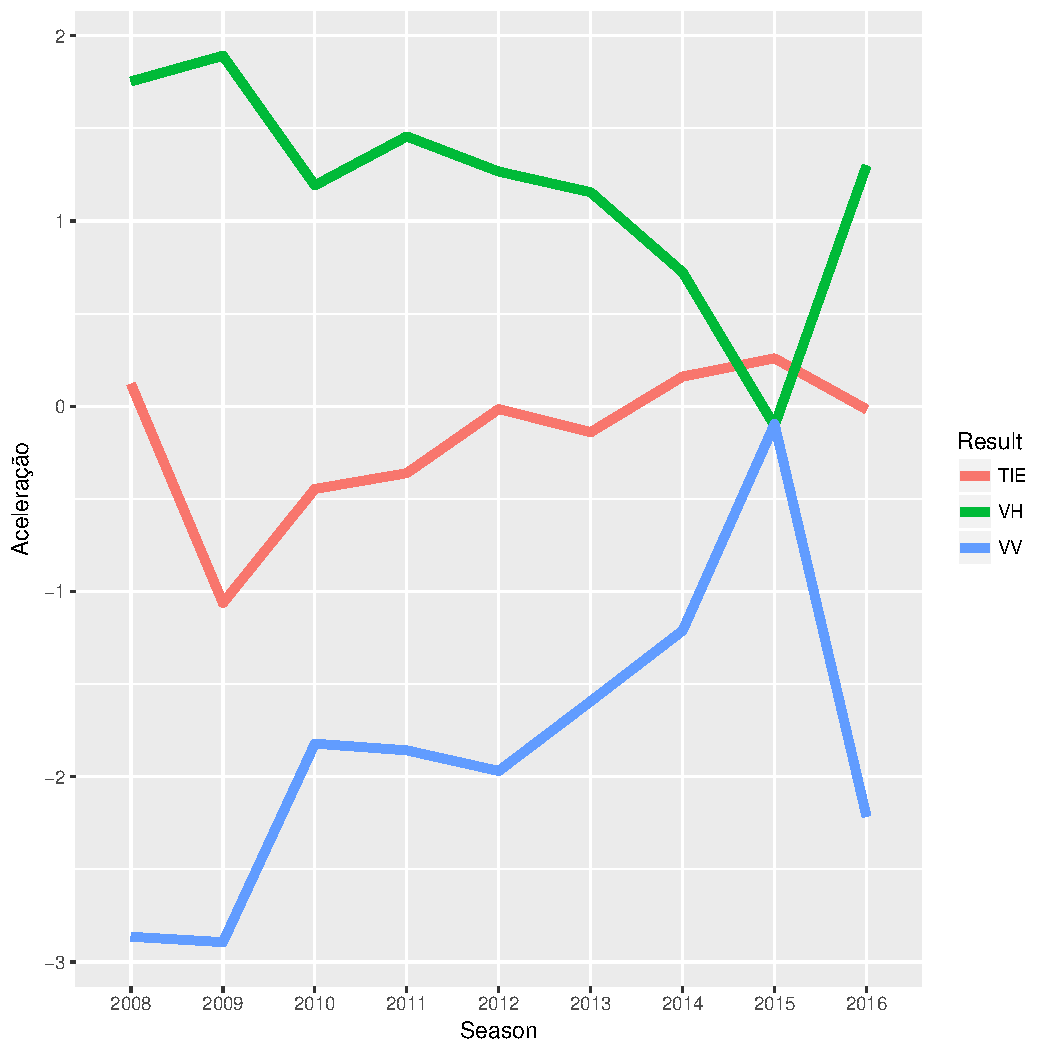
\includegraphics[width=5cm,height=4cm]{aceleracao_result.pdf} }}%
    \qquad
    \subfloat[\scriptsize{Acceleration mensure for period of analysis.}]{{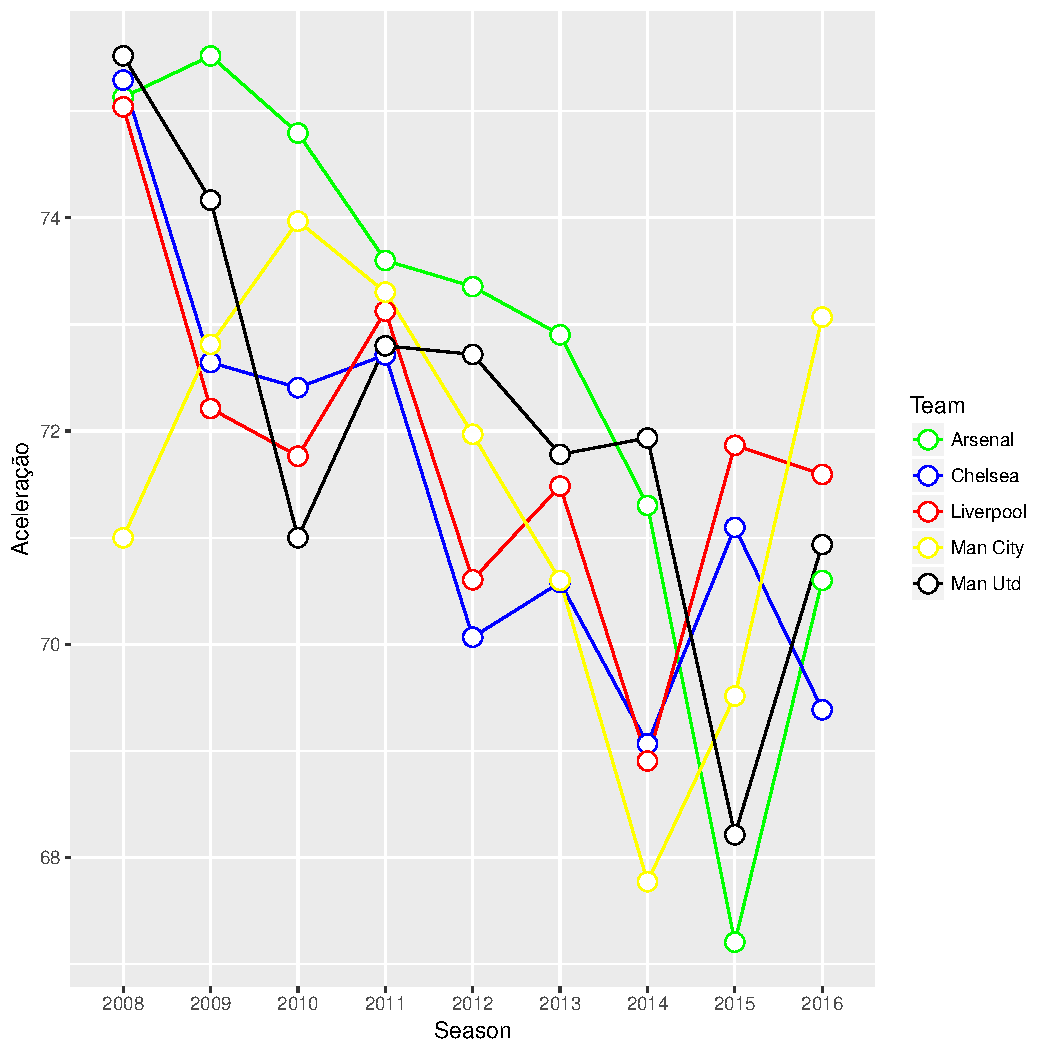
\includegraphics[width=5cm,height=4cm]{aceleracao_descri.pdf} }}%
    \caption[\scriptsize{Summary acceleration mensure.}]{\scriptsize{ \textbf{(a)} Summary acceleration mensures by match result. Tie (TIE), Victory of Home team (VH) and Victory of visitor team (VV). \textbf{(b)} Skill acceleration mensure for period of analysis. }}
    \label{fig:summary}%
\end{figure}


Seja $X^{home}_{r}$ o valor da veriável regressora $r$ para o time mandante do confronto e, analogamente, $X^{visitor}_{r}$ o valor para a mesma variável do time visitante. A equação do modelo \ref{eq:g} é modelada pela diferença entre a habilidade na variável $r$ entre o time mandante e o visitante. $X_{r} = X^{home}_{r}-X^{visitor}_{r}$. Dessa forma, valores muito positivos para a variável $X_{r}$ significam superioridade do time mandante e os negativos significam que as habilidades do time visitante são superiores aos anfitriões.


O gráfico do painel $(a)$ da imagem \ref{fig:summary} mostra que, em média, os jogos em que a medida $X_r$ é maior do que zero, houve vitória do time mandante. Do forma similar, nos casos em que $X_r$ foi menor do que zero o time visitante venceu. Os casos tem empate, há equilíbrio entre os times e a medida $X_r$ é próxima, em média, de zero. Em anexo estão as medidas para as demais variáveis.

O gráfico do painel $(b)$ da imagem \ref{fig:summary} mostra a evolução da variável aceleração ao longo do período de análise para os principais times da \textit{Premier League}. É possível perceber que todos times tiveram entre $2008$ e $2014$ uma diminuição do valor médio da variável aceleração. O processo de renovação de elenco do Chelsea, Liverpool e Mancherster City iniciou-se em $2015$. Já para Arsenal e Mancherster United a renovação ocorreu no ano seguinte em $2015$.

O início de renovação do Chelse foi campeã pode ajudar a explicar o sucesso em $2015$ e $2017$. Uma queda dessas e outras informações das equipes inglesas podem ajudar a compreender a zebra de $2016$, quando a equipe de pouca expressão Leicester foi campeã. 

Pretendemos explicar e predizer o resultado dos jogos da Premier League, baseado nas habilidades auferidas pelo site FIFA dos jogadores de cada time.


A relação positiva é observada quando o aumentoda  variável regressora $X_r$, que representa o nível de superioridade do time mandante, contribui para a vitória do time mandante. Nesse raciocínio, é esperado nos jogos em que houve vitória do time mandante, a média dessa variável é maior do que os valores dos jogos empate, que por sua vez é maior do que os que ocorreram derrota. $\bar{X}_r^{VH}\geq \bar{X}_r^{Tie} \geq \bar{X}_r^{VV}$

 De maneira análoga, a relação negativa é observada quando o diminuição de $X_r$ contribui para a derrota do time mandante. Nesse caso, é esperado que nos jogos em que houve vitória do time mandante, a média dessa variável é menor do que os valores dos jogos empate, que por sua vez é menor do que os que ocorreram derrota. $\bar{X}_r^{VH} \leq \bar{X}_r^{Tie} \leq \bar{X}_r^{VV}$

Além desse resultado geral, é esperado que ao longo de \textbf{cada temporadas analisadas} esse comportamento se repita. O número de vezes em que esse resultado é observado pode sugerir o nível dessa relação.


A tabela \ref{tab:selectvar} apresenta essas análises paras cada variável e dá indícios para o processo de seleção das variáveis relevantes para o modelo. É possível identificar, que as variáveis ``chute de longe" e ``controle de bola" um comportamento adequado com a relação positiva. Também é possível notar que as variáveis ``idade" e ``classificação na tabela" têm relação negativa com a vitória do mandante.

% latex table generated in R 3.3.2 by xtable 1.8-2 package
% Thu Nov 16 02:41:35 2017
\begin{table}[ht]
\begin{small}
\begin{tabular}{l||rrr||rrr|r|||rrr||r}
  \hline
     \hline
\rowcolor{SeaGreen3!30!} & \multicolumn{3}{c||}{Média} &   \multicolumn{4}{c|||}{Indicador positivo} & \multicolumn{4}{c}{Indicador negativo} \\
\hline 
  \hline
\rowcolor{SeaGreen3!30!} Skill &  $\bar{X}_r^{VH}$ &  $\bar{X}_r^{TIE}$ &  $\bar{X}_r^{VV}$ & NVH & NVV & NTIE & \textbf{NP }& NVH & NVV & NTIE & \textbf{NN }\\ 
 \hline
\rowcolor{gray!30!} Aceleração & 1.173 & -0.095 & -1.748 & 88.9 & 88.9 & 88.9 & 88.9 & 11.1 & 0.0 & 0.0 & 11.1 \\ 
\rowcolor{gray!10!}  Altura & 0.036 & -0.017 & -0.052 & 33.3 & 44.4 & 22.2 & 33.3 & 11.1 & 33.3 & 0.0 & 11.1 \\ 
\rowcolor{gray!30!}   Cabeceio & 0.458 & -0.202 & -0.557 & 66.7 & 66.7 & 55.6 & 66.7 & 0.0 & 22.2 & 0.0 & 0.0 \\ 
\rowcolor{gray!10!}   Carrinho & 0.549 & -0.015 & -0.852 & 77.8 & 77.8 & 66.7 & 77.8 & 0.0 & 11.1 & 0.0 & 0.0 \\ 
 \rowcolor{gray!30!}  Ch. de longe & 1.266 & -0.236 & -1.781 & 100.0 & 88.9 & 88.9 & 100.0 & 0.0 & 0.0 & 0.0 & 0.0 \\ 
\rowcolor{gray!10!}   Cobr. falta & 1.240 & -0.095 & -1.878 & 88.9 & 88.9 & 77.8 & 88.9 & 0.0 & 0.0 & 0.0 & 0.0 \\ 
 \rowcolor{gray!30!}  Combativ. & 0.479 & -0.307 & -0.513 & 77.8 & 66.7 & 55.6 & 77.8 & 11.1 & 11.1 & 11.1 & 11.1 \\ 
\rowcolor{gray!10!}   Contr. bola & 1.644 & -0.402 & -2.234 & 100.0 & 88.9 & 88.9 & 100.0 & 0.0 & 0.0 & 0.0 & 0.0 \\ 
\rowcolor{gray!30!}   Cruzamento & 1.651 & -0.475 & -2.181 & 100.0 & 88.9 & 88.9 & 100.0 & 0.0 & 0.0 & 0.0 & 0.0 \\ 
\rowcolor{gray!10!}   Div. em pé & 0.630 & -0.040 & -0.958 & 88.9 & 88.9 & 77.8 & 88.9 & 0.0 & 0.0 & 0.0 & 0.0 \\ 
\rowcolor{gray!30!}   Dribles & 1.587 & -0.220 & -2.306 & 100.0 & 88.9 & 88.9 & 100.0 & 0.0 & 0.0 & 0.0 & 0.0 \\ 
\rowcolor{gray!10!}   Dur. contrato & 0.419 & -0.151 & -0.535 & 100.0 & 88.9 & 88.9 & 100.0 & 0.0 & 0.0 & 0.0 & 0.0 \\ 
\rowcolor{gray!30!}   Elast. GL & 0.205 & -0.032 & -0.302 & 66.7 & 55.6 & 33.3 & 66.7 & 11.1 & 11.1 & 11.1 & 11.1 \\ 
\rowcolor{gray!10!}   Finalização & 0.720 & -0.047 & -1.091 & 77.8 & 77.8 & 77.8 & 77.8 & 22.2 & 11.1 & 11.1 & 22.2 \\ 
\rowcolor{gray!30!}   Fôlego & 0.405 & -0.087 & -0.567 & 55.6 & 66.7 & 55.6 & 55.6 & 33.3 & 22.2 & 22.2 & 33.3 \\ 
\rowcolor{gray!10!}   Força & 0.247 & 0.049 & -0.445 & 33.3 & 88.9 & 33.3 & 33.3 & 11.1 & 11.1 & 11.1 & 11.1 \\ 
\rowcolor{gray!30!}   Força chute & 1.255 & -0.447 & -1.577 & 88.9 & 88.9 & 88.9 & 88.9 & 0.0 & 11.1 & 0.0 & 0.0 \\ 
\rowcolor{gray!10!}   Idade & -0.258 & 0.039 & 0.364 & 0.0 & 0.0 & 0.0 & 0.0 & 100.0 & 100.0 & 100.0 & 100.0 \\ 
\rowcolor{gray!30!}   Lançamento & 1.761 & -0.165 & -2.630 & 100.0 & 100.0 & 100.0 & 100.0 & 0.0 & 0.0 & 0.0 & 0.0 \\ 
\rowcolor{gray!10!}   Manejo & -0.254 & 0.187 & 0.239 & 44.4 & 44.4 & 44.4 & 44.4 & 55.6 & 55.6 & 55.6 & 55.6 \\ 
\rowcolor{gray!30!}   Marcação & 0.618 & -0.251 & -0.757 & 88.9 & 88.9 & 77.8 & 88.9 & 0.0 & 0.0 & 0.0 & 0.0 \\ 
\rowcolor{gray!10!}   Passe curto & 1.756 & -0.308 & -2.494 & 100.0 & 88.9 & 88.9 & 100.0 & 0.0 & 0.0 & 0.0 & 0.0 \\ 
 \rowcolor{gray!30!}  Perna boa & 0.019 & 0.010 & -0.044 & 33.3 & 33.3 & 22.2 & 33.3 & 55.6 & 22.2 & 22.2 & 55.6 \\ 
\rowcolor{gray!10!}   Perna ruim & 0.223 & 0.039 & -0.390 & 66.7 & 100.0 & 66.7 & 66.7 & 0.0 & 0.0 & 0.0 & 0.0 \\ 
 \rowcolor{gray!30!}  Peso & 0.036 & -0.017 & -0.052 & 33.3 & 44.4 & 22.2 & 33.3 & 11.1 & 33.3 & 0.0 & 11.1 \\ 
\rowcolor{gray!10!}   Pique & 1.092 & -0.082 & -1.641 & 100.0 & 100.0 & 100.0 & 100.0 & 0.0 & 0.0 & 0.0 & 0.0 \\ 
\rowcolor{gray!30!}   Posição & -2.263 & 1.113 & 3.310 & 0.0 & 0.0 & 0.0 & 0.0 & 100.0 & 100.0 & 100.0 & 100.0 \\ 
 \rowcolor{gray!10!}  Posicion. GL & -0.264 & 0.165 & 0.267 & 22.2 & 33.3 & 22.2 & 22.2 & 66.7 & 55.6 & 55.6 & 66.7 \\ 
 \rowcolor{gray!30!}  Reação & 1.647 & -0.450 & -2.218 & 100.0 & 100.0 & 100.0 & 100.0 & 0.0 & 0.0 & 0.0 & 0.0 \\ 
\rowcolor{gray!10!}   Reflexos & -0.288 & 0.246 & 0.239 & 33.3 & 33.3 & 33.3 & 33.3 & 66.7 & 55.6 & 55.6 & 66.7 \\ 
   \hline
      \hline
\end{tabular}
\end{small}	
\caption[\scriptsize{Variable selection.}]{\scriptsize{ Tabela indicativa do tipo de relação entre a habilidade dos times e o resultado do jogo. Na seção positiva, a coluna VH apresenta a proporção de temporadas em que o valor médio da habilidade para os casos em que o time mandante venceu foi superior às médias dos casos de empate e derrota, indicando uma relação \textbf{positiva} entre a variável $X_r$ (superioridade do time mandante) e vitória do mandante. Na seção negativa, essa mesma coluna apresenta a proporção de temporadas em que o valor médio da habilidade foi \textbf{inferior} às médias de empate e derrota. De maneira análoga, nesse seção essa coluna indica uma relação \textbf{negativa} entre a variável $X_r$. Na seção positiva, a coluna Tie apresenta a proporção de temporadas em que o valor médio da habilidade foi superior às médias de empate e derrota, indicando uma relação \textbf{positiva} entre a variável $X_r$. A coluna TIE apresenta a proporção de temporadas em que o valor médio da habilidade foi superior às médias de empate e derrota.  }}
    \label{tab:selectvar}%
\end{table}


\section{Método}
\label{sec:metodo}

A base de dados foi dividia em:
\begin{itemize}
\item \textbf{base de treino:} jogos das temporadas de $2008$ e $2014$. A base servirá para estimar os parâmetros do modelo da equação \ref{eq:g}.
\item \textbf{base de tuning:} jogos das temporadas de $2015$. A base servirá para estimar os parâmetros $\lambda$ e $\phi$ do processo de \textbf{regularização} na equação \ref{eq:vero}.
\item \textbf{base de teste:} jogos das temporadas de $2016$. A base servirá para avaliar $out-of-sample$ o modelo.
\end{itemize}


Os parâmetros de $\phi$ e $\lambda$ foram avalidados por meio do \textit{grid-search}, sendo $\phi = (0 , 0.1,0.2,0.3,\cdots,0.9,1)$ e  $\lambda =( 0,0.5,1,1.5,2,2.5,3)$. Os gráficos da figura \ref{fig:tunning} apresentam o desempenho do modelo para o \textit{grid} de procura dos parâmetros.


\begin{figure}%
    \centering
    \subfloat[\scriptsize{Tunning surface parameters}]{{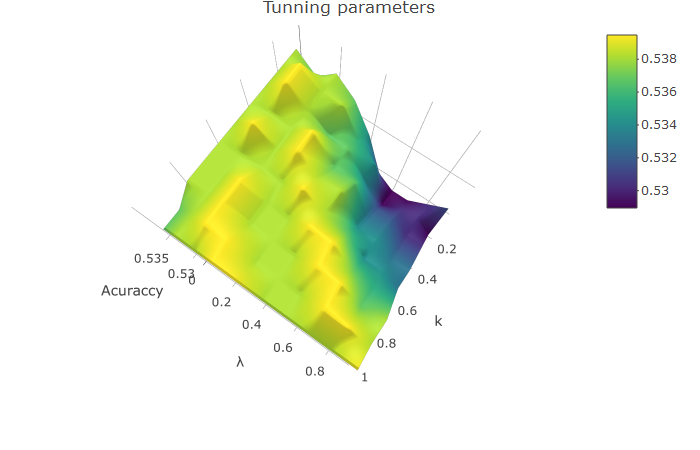
\includegraphics[width=5cm,height=4cm]{tunning_all.png} }}%
    \qquad
    \subfloat[\scriptsize{Tunning contour parameters }]{{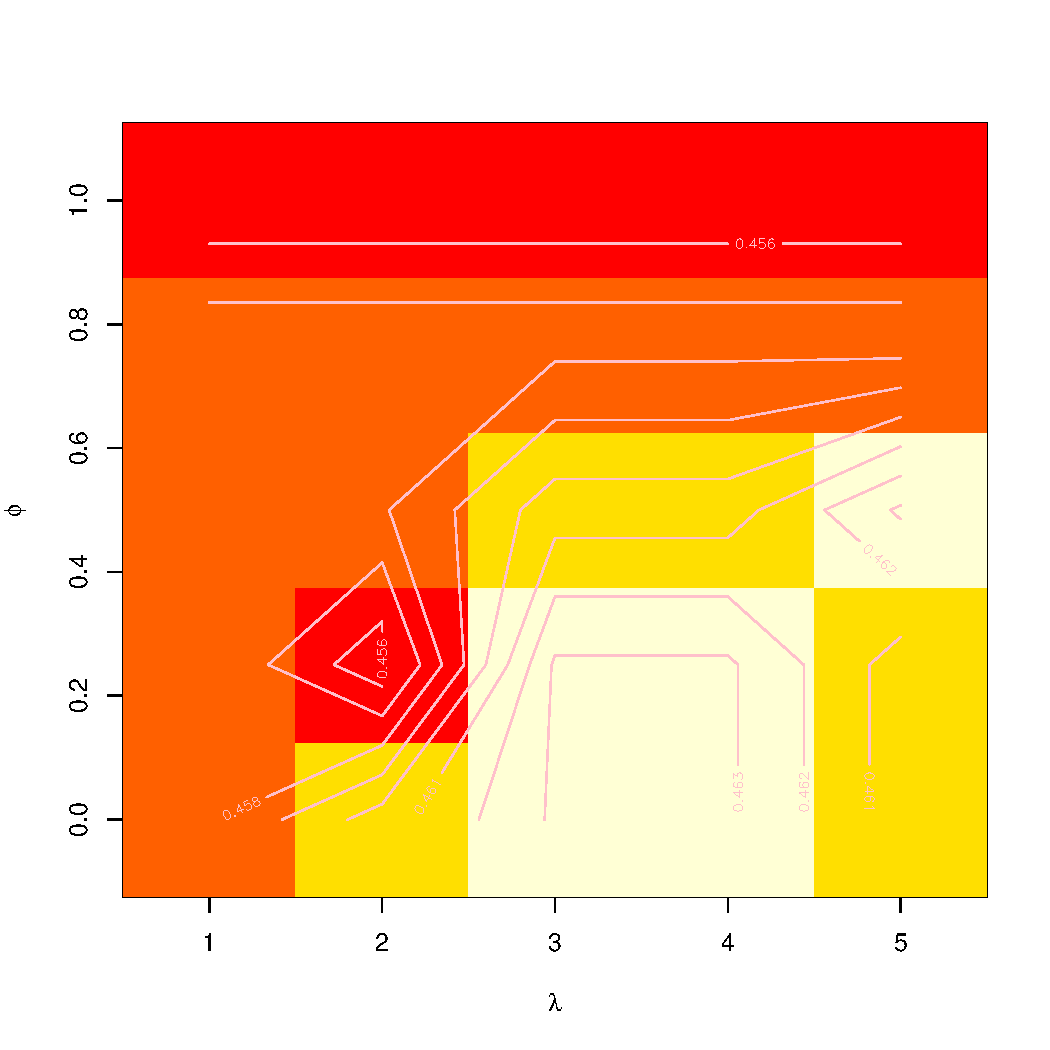
\includegraphics[width=5cm,height=4cm]{contour_dissimilaridade.pdf} }}%
    \caption[\scriptsize{Tunning parameters.}]{\scriptsize{ \textbf{(a)} Surface of parameters $\lambda$ and $k$ related with equation \ref{eq:vero}.\textbf{(b)}Contour of parameters $\lambda$ and $k$ related with equation \ref{eq:vero}.}}
    \label{fig:tunning}%
\end{figure}


\subsection{Modelo 1}
\label{sec:mod1}

O modelo 1 utiliza todas as variáveis disponíveis e utiliza medida de dissimilaridade para empate, vitória ou derrota do time visitante.



O resultado para o modelo proposto não consegue identificar os resultados empate.

% latex table generated in R 3.3.2 by xtable 1.8-2 package
% Tue Nov 14 17:00:59 2017
\begin{table}[ht]
\centering
\begin{tabular}{crrrr}
  \hline
Seasons & Global & Home & Tie & Visitor \\ 
  \hline
2008-2014 & 47.11 & 79.65 & 0.00 & 36.52 \\ 
  2015 & 38.95 & 73.25 & 0.00 & 28.45 \\ 
  2016 & 56.32 & 85.56 & 0.00 & 49.54 \\ 
   \hline
\end{tabular}
    \caption[\scriptsize{Medidas do modelo.}]{\scriptsize{Medidas do modelo. A coluna Global é a acurácia geral para o modelo. A coluna Home, Tie e Visitor apresentam os valores da acurácia para os casos de vitória, empate e derrota do time mandante, respectivamente.}}
    \label{tab:medidasmod}
\end{table}


A tabela \ref{tab:forecastdissi} apresenta a simulação para o resultado da temporada de 2017/2018 baseada nos parâmetros estimados.


% latex table generated in R 3.3.2 by xtable 1.8-2 package
% Sun Nov 12 15:31:54 2017
\begin{table}[ht]
\centering
\begin{tabular}{lrrrr}
  \hline
Team & PLC & CCL& CEL & RET \\ 
  \hline
Man Utd & 16.50 & 49.02 & 14.96 & 1.77 \\ 
  Man City & 16.08 & 48.46 & 14.94 & 1.58 \\ 
  Tottenham & 12.90 & 43.01 & 15.79 & 1.98 \\ 
  Chelsea & 10.99 & 37.00 & 14.25 & 3.62 \\ 
  Arsenal & 9.32 & 35.04 & 14.77 & 3.83 \\ 
  Southampton & 8.70 & 36.16 & 14.13 & 3.08 \\ 
  Newcastle & 4.51 & 22.01 & 12.36 & 7.78 \\ 
  Crystal Palace & 3.85 & 19.93 & 11.86 & 9.30 \\ 
  Stoke City & 3.31 & 17.91 & 11.30 & 9.36 \\ 
  Everton & 2.79 & 16.15 & 10.55 & 11.90 \\ 
  Leicester & 1.85 & 10.63 & 8.78 & 16.67 \\ 
  Liverpool & 1.77 & 12.71 & 8.93 & 14.09 \\ 
  Watford & 1.69 & 9.36 & 7.82 & 16.87 \\ 
  West Brom & 1.52 & 10.38 & 8.18 & 17.85 \\ 
  Bournemouth & 1.52 & 8.61 & 7.53 & 19.35 \\ 
  Swansea & 1.14 & 8.78 & 7.97 & 19.50 \\ 
  Burnley & 0.60 & 4.68 & 5.03 & 29.40 \\ 
  West Ham & 0.46 & 4.25 & 4.81 & 31.67 \\ 
  Brighton & 0.40 & 4.31 & 4.06 & 32.00 \\ 
  Huddersfield & 0.10 & 1.62 & 1.98 & 48.40 \\ 
   \hline
\end{tabular}
    \caption[\scriptsize{TAVB}]{\scriptsize{Detailed table of competition where the values are probability of the simulation. Premier League Champion (PLC), Classify to UEFA Champions League (CCL), Classify to UEFA Europa League (CEL) Relegated team (RE).}}
    \label{tab:forecastdissi}
\end{table}


\newpage

\subsection{Modelo 2}
\label{sec:mod2}

O modelo 2 adiciona medida de similaridade para modelar o empate.


Isso ocorre devido o valor de $X_r$ representar uma medida de \textbf{dissimilaridade}, isto é, quanto maior o valor $X_r$ mais diferente são as habilidades do time mandante e visitante. Caso as habilidades dos dois times sejam iguais o valor  $X_r$ zera, inviabilizando a regressão do parâmetro $\alpha_{Tie}$. 

Dessa forma, propomos uma medida de \textbf{similaridade} para regressão do parâmetro $\alpha_{Tie}$ relativo ao empate. Faremos:

\begin{equation}
X_r^{Tie} = \gamma \exp{\left\{-\sigma X_r ^2\right\}}
\label{eq:transform}
\end{equation}

Nessa estratégia, os parâmetros $\lambda$, $\phi$, $\sigma$ e $\gamma$ são determinados utilizando a procedimento \textit{tuning}. O modelo para $\alpha_{Tie}$ captará o nível de similaridade dos times.


% latex table generated in R 3.3.2 by xtable 1.8-2 package
% Tue Nov 14 19:42:00 2017
\begin{table}[ht]
\centering
\begin{tabular}{cc|r|rrr}
  \hline
Seasons & Data & \textbf{Global} & Home & Tie & Visitor \\ 
  \hline
2008-2014 & Trainning & 56.97 & 80.91 & 8.77 & 56.30 \\ 
  2015 & Tuning & 44.21 & 71.34 & 3.74 & 44.83 \\ 
  2016 & Test & 51.05 & 66.84 & 4.76 & 59.63 \\ 
   \hline
\end{tabular}
    \caption[\scriptsize{Medidas do modelo com similaridade para o empate.}]{\scriptsize{Medidas do modelo que inclue o ajuste para similaridade do empate. A coluna Global é a acurácia geral para o modelo. A coluna Home, Tie e Visitor apresentam os valores da acurácia para os casos de vitória, empate e derrota do time mandante, respectivamente. }}
    \label{tab:medidasmodsi}
\end{table}	



% latex table generated in R 3.3.2 by xtable 1.8-2 package
% Sun Nov 12 15:31:54 2017
\begin{table}[ht]
\centering
\begin{tabular}{lrrrr}
  \hline
Team & PLC & CCL& CEL & RET \\ 
  \hline
  Liverpool & 39.00 & 86.00 & 7.00 & 0.00 \\ 
  Man City & 31.00 & 78.00 & 12.00 & 0.00 \\ 
  Chelsea & 13.00 & 62.00 & 17.00 & 0.00 \\ 
  Leicester & 6.00 & 34.00 & 24.00 & 0.00 \\ 
  Tottenham & 5.00 & 32.00 & 24.00 & 2.00 \\ 
  Man Utd & 4.00 & 26.00 & 19.00 & 0.00 \\ 
  Stoke City & 1.00 & 26.00 & 26.00 & 0.00 \\ 
  Everton & 1.00 & 14.00 & 8.00 & 3.00 \\ 
  West Ham & 0.00 & 9.00 & 13.00 & 10.00 \\ 
  West Brom & 0.00 & 11.00 & 17.00 & 4.00 \\ 
  Watford & 0.00 & 0.00 & 3.00 & 21.00 \\ 
  Swansea & 0.00 & 1.00 & 5.00 & 17.00 \\ 
  Southampton & 0.00 & 6.00 & 6.00 & 16.00 \\ 
  Newcastle & 0.00 & 3.00 & 3.00 & 9.00 \\ 
  Huddersfield & 0.00 & 0.00 & 0.00 & 64.00 \\ 
  Crystal Palace & 0.00 & 1.00 & 5.00 & 21.00 \\ 
  Burnley & 0.00 & 0.00 & 0.00 & 84.00 \\ 
  Brighton & 0.00 & 2.00 & 1.00 & 18.00 \\ 
  Bournemouth & 0.00 & 0.00 & 1.00 & 27.00 \\ 
  Arsenal & 0.00 & 9.00 & 9.00 & 4.00 \\ 
   \hline
\end{tabular}
    \caption[\scriptsize{TAVB} with similarity]{\scriptsize{Detailed table of competition where the values are probability of the simulation with similarity for tie. Premier League Champion (PLC), Classify to UEFA Champions League (CCL), Classify to UEFA Europa League (CEL) Relegated team (RE).}}
    \label{tab:forecastsi}
\end{table}

Apesar de pequena, o tratamento para a regressão do coeficiente do empate contribui para melhorar o poder de previsibilidade do modelo. 


A tabela \ref{tab:selectvartrans} apresenta as medidas descritivas utilizando a transformação \ref{eq:transform} com parâmetro $\gamma=1$ e $\sigma=1$.

% latex table generated in R 3.3.2 by xtable 1.8-2 package
% Thu Nov 16 13:58:52 2017
\begin{table}[ht]
\begin{small}
\begin{tabular}{l||rrr||cc|||c}
  \hline
     \hline
\rowcolor{SeaGreen3!30!} & \multicolumn{3}{c||}{Média} &   \multicolumn{2}{c||||}{Indicador positivo} & \multicolumn{1}{c}{Indicador negativo} \\
\hline 
  \hline
\rowcolor{SeaGreen3!30!} Skill &  $\bar{X}_r^{VH}$ &  $\bar{X}_r^{TIE}$ &  $\bar{X}_r^{VV}$ & \textbf{MNP } & \textbf{NP }& \textbf{NN }\\ 
 \hline
\rowcolor{gray!30!} Aceleração & 0.253 & 0.991 & 0.047 & 1.304 & 88.9 & 11.1 \\ 
\rowcolor{gray!10!} Altura & 0.999 & 1.000 & 0.997 & -0.030 & 22.2 & 77.8 \\ 
\rowcolor{gray!30!} Cabeceio & 0.811 & 0.960 & 0.733 & 0.245 & 55.6 & 44.4 \\ 
\rowcolor{gray!10!} Carrinho & 0.740 & 1.000 & 0.484 & 0.650 & 66.7 & 33.3 \\ 
\rowcolor{gray!30!} Ch. de longe & 0.201 & 0.946 & 0.042 & 1.000 & 88.9 & 11.1 \\ 
\rowcolor{gray!10!} Cobr. falta & 0.215 & 0.991 & 0.029 & 1.135 & 77.8 & 22.2 \\ 
\rowcolor{gray!30!} Combativ. & 0.795 & 0.910 & 0.769 & 0.162 & 55.6 & 44.4 \\ 
\rowcolor{gray!10!} Contr. bola & 0.067 & 0.851 & 0.007 & 1.204 & 88.9 & 11.1 \\ 
\rowcolor{gray!30!} Cruzamento & 0.066 & 0.798 & 0.009 & 1.042 & 88.9 & 11.1 \\ 
\rowcolor{gray!10!} Div. em pé & 0.673 & 0.998 & 0.399 & 0.755 & 77.8 & 22.2 \\ 
\rowcolor{gray!30!} Dribles & 0.081 & 0.953 & 0.005 & 1.511 & 88.9 & 11.1 \\ 
\rowcolor{gray!10!} Duração Do Contrato & 0.839 & 0.978 & 0.751 & 0.346 & 88.9 & 11.1 \\ 
\rowcolor{gray!30!} Elast. GL & 0.959 & 0.999 & 0.913 & 0.121 & 44.4 & 55.6 \\ 
\rowcolor{gray!10!} Finalização & 0.596 & 0.998 & 0.304 & 0.958 & 88.9 & 11.1 \\ 
\rowcolor{gray!30!} Fôlego & 0.849 & 0.993 & 0.725 & 0.560 & 77.8 & 22.2 \\ 
\rowcolor{gray!10!} Força & 0.941 & 0.998 & 0.820 & 0.157 & 44.4 & 55.6 \\ 
\rowcolor{gray!30!} Força chute & 0.207 & 0.819 & 0.083 & 0.930 & 88.9 & 11.1 \\ 
\rowcolor{gray!10!} Idade & 0.936 & 0.999 & 0.876 & 0.225 & 100.0 & 0.0 \\ 
\rowcolor{gray!30!} Lançamento & 0.045 & 0.973 & 0.001 & 1.459 & 100.0 & 0.0 \\ 
\rowcolor{gray!10!} Manejo & 0.937 & 0.966 & 0.944 & 0.397 & 100.0 & 0.0 \\ 
\rowcolor{gray!30!} Marcação & 0.683 & 0.939 & 0.564 & 0.453 & 77.8 & 22.2 \\ 
\rowcolor{gray!10!} Passe curto & 0.046 & 0.910 & 0.002 & 1.296 & 88.9 & 11.1 \\ 
\rowcolor{gray!30!} Perna boa & 1.000 & 1.000 & 0.998 & 0.000 & 55.6 & 44.4 \\ 
\rowcolor{gray!10!} Perna ruim & 0.951 & 0.998 & 0.859 & 0.155 & 55.6 & 44.4 \\ 
\rowcolor{gray!30!} Peso & 0.999 & 1.000 & 0.997 & -0.030 & 22.2 & 77.8 \\ 
\rowcolor{gray!10!} Pique & 0.303 & 0.993 & 0.068 & 1.296 & 100.0 & 0.0 \\ 
\rowcolor{gray!30!} pos & 0.006 & 0.289 & 0.000 & 0.580 & 88.9 & 11.1 \\ 
\rowcolor{gray!10!} Posicion. GL & 0.933 & 0.973 & 0.931 & 0.408 & 77.8 & 22.2 \\ 
\rowcolor{gray!30!} Reação & 0.066 & 0.817 & 0.007 & 1.218 & 100.0 & 0.0 \\ 
\rowcolor{gray!10!} Reflexos & 0.920 & 0.941 & 0.945 & 0.453 & 88.9 & 11.1 \\ 
   \hline
\end{tabular}
\end{small}
\caption[\scriptsize{Variable selection with transformation.}]{\scriptsize{ Tabela indicativa do tipo de relação entre a habilidade dos times e o resultado do jogo com ênfase no resultado de empate. A interpretação é similar àquela realizada na tabela \ref{tab:selectvar}. A transformação \ref{eq:transform} permite que o efeito de similaridade das habilidades esperado para os resultados de empate seja captado. Essa transformação é exclusiva para a regressão do parâmetro $\alpha_{Tie}$. $ MNP = 2  \bar{X}_r^{TIE} - \bar{X}_r^{VH} - \bar{X}_r^{VV}$ é o valor médio para a superioridade da similaridade do empate, variando entre $-2$ e $2$. Valos próximos de $2$ indicam que a variável possui nível de \textbf{similaridade máxima} das habilidades dos times nos empates e \textbf{similaridade mínima} para os casos de vitória ou derrota do mandante. A coluna NP indica a proporção de temporadas em que o o valor do regressor transformado foi superior nos resultados de empate quando comparada com vitória e derrota do time mandante. O coluna NN representa indica a proporção de temporadas em que o valor do regressor transformado foi inferior nos resultados de empate quando comparada ou com vitória ou com derrota do time mandante. A primeira medida indica a  consistência do método para modelar o empate e a segunda inconsistência.}}
    \label{tab:selectvartrans}
\end{table}

A tabela \ref{tab:selectvartrans} dá indícios de que as variáveis ``A"


\newpage
\subsection{Modelo 3}
\label{sec:mod3}

O modelo 3 restringe as variáveis baseado nas análise preliminares do modelo 1 e 2.

O primeiro critério seleciona as variáveis para modelar a vitória e a derrota do time mandante. A partir da tabela \ref{tab:selectvar} foram selecionados aqueles que possuem a variável NP e NN com valor superior ou igual a $80\%$, isso é, variáveis que possuem relação positiva ou negativa em mais de $80\%$ das temporadas.

A figura \ref{fig:medresumo} destaca as variáveis selecionadas.


\begin{figure}
\begin{tabular}{ccccc}
  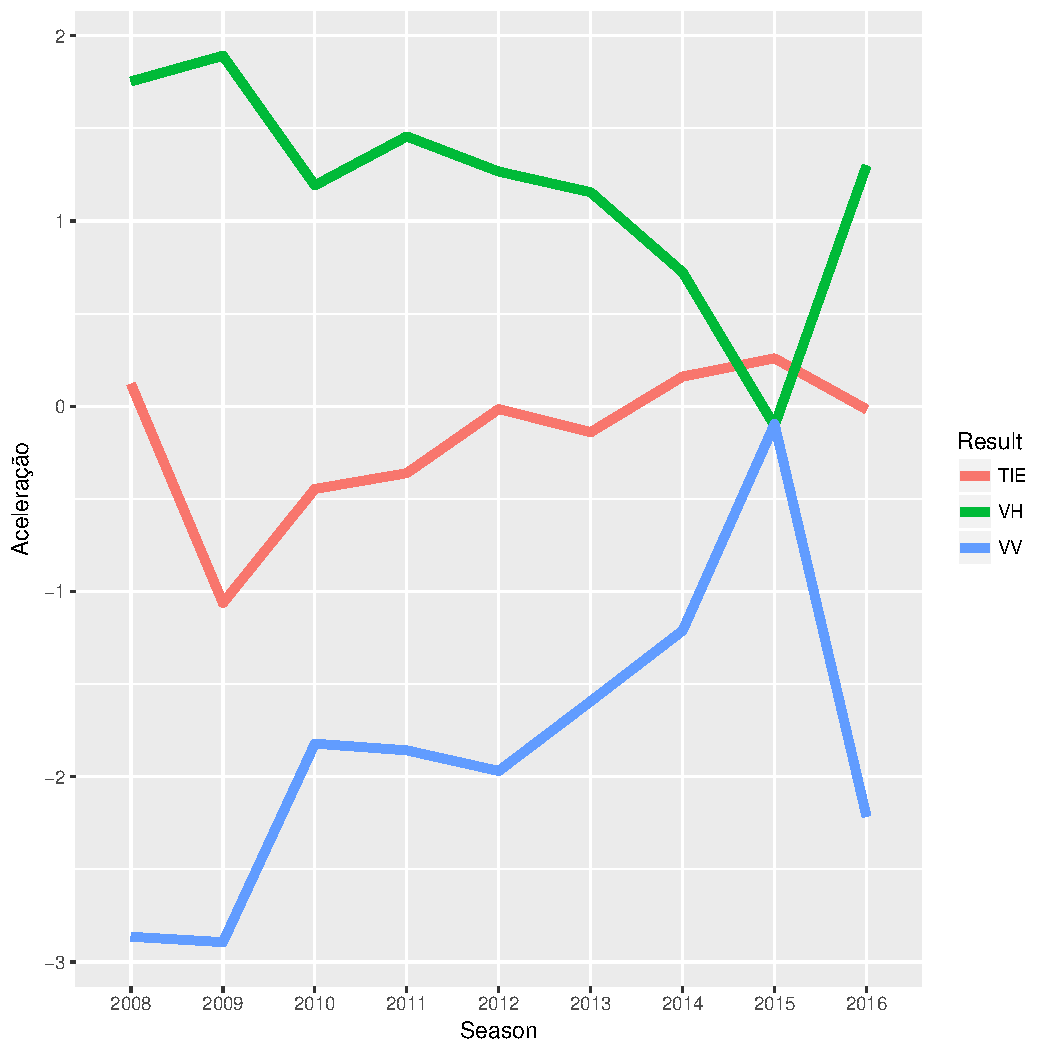
\includegraphics[width=25mm]{aceleracao_result} & 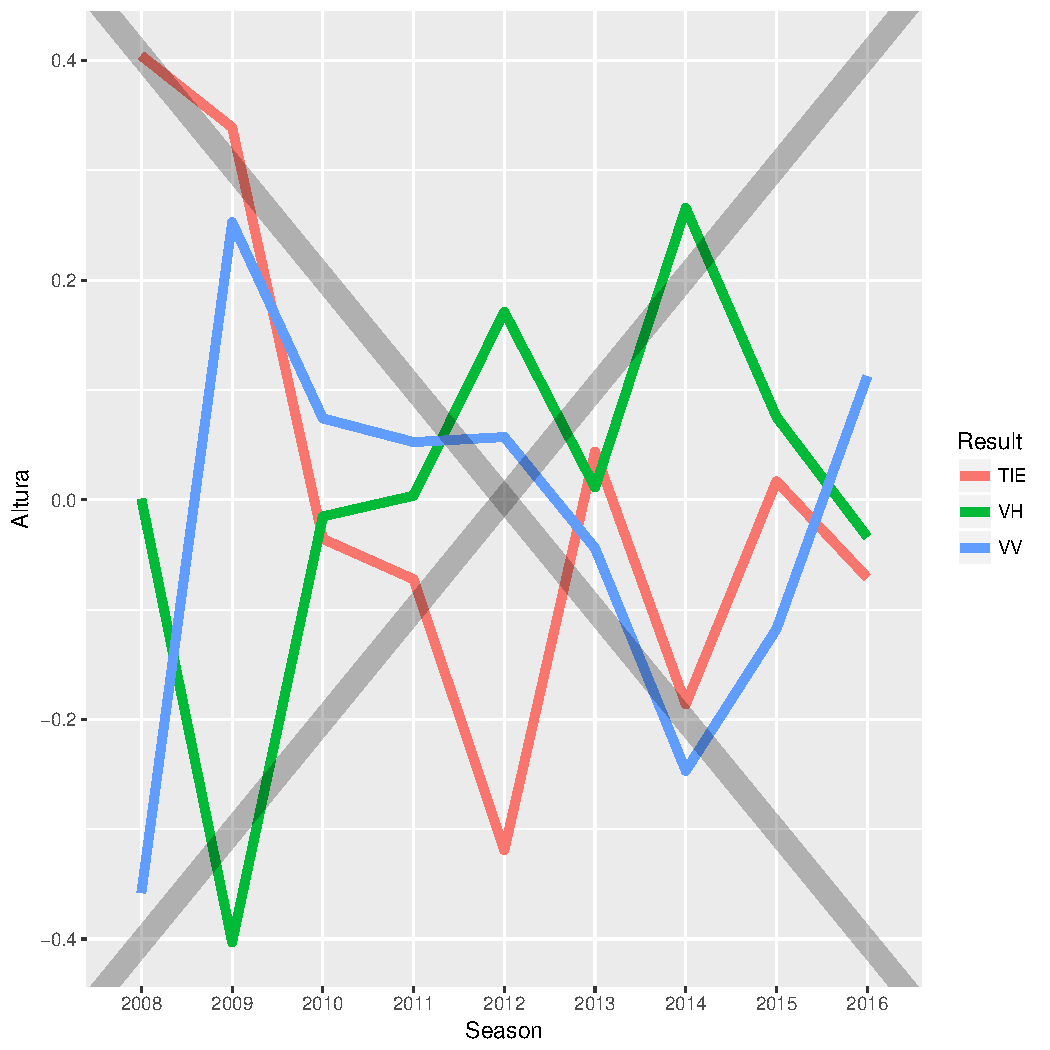
\includegraphics[width=25mm]{altura_result} & 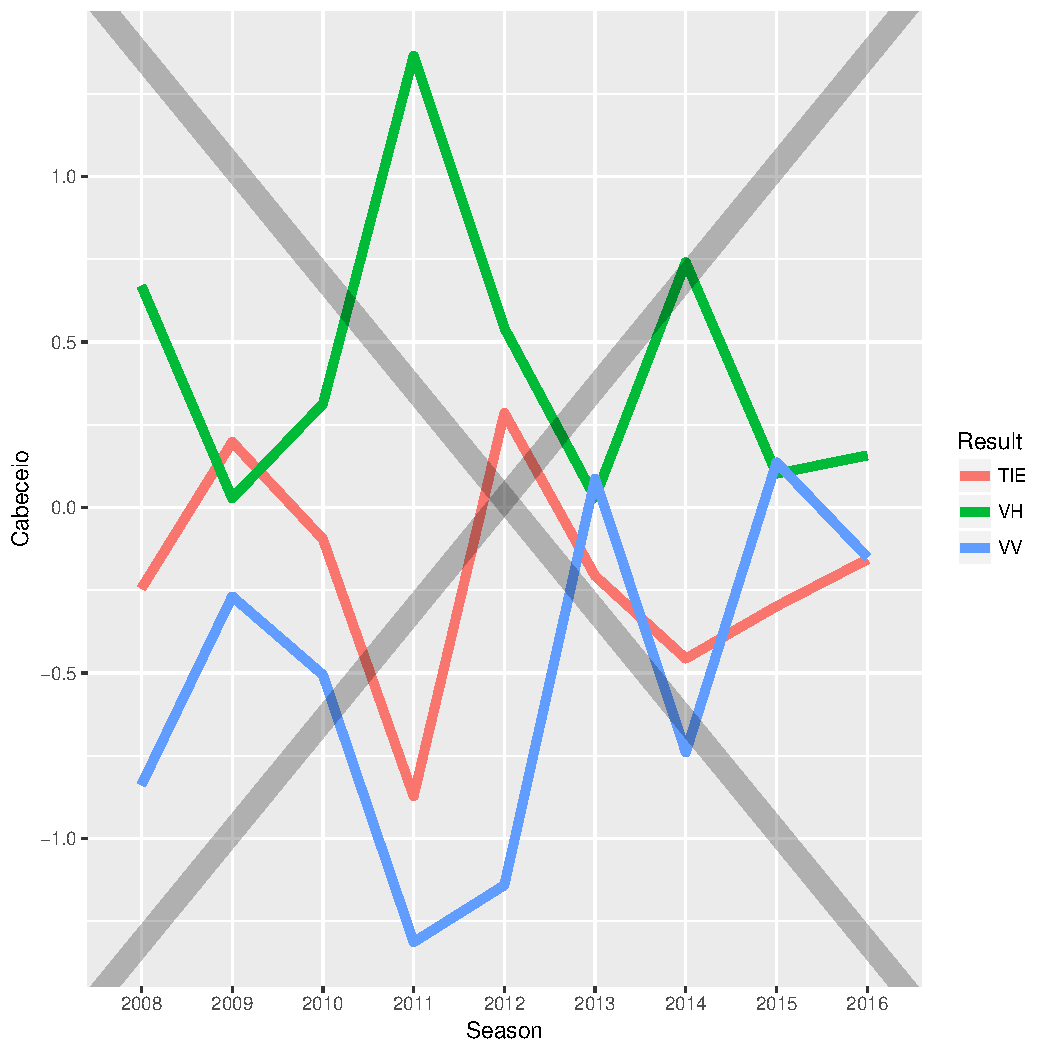
\includegraphics[width=25mm]{cabeceio_result} &   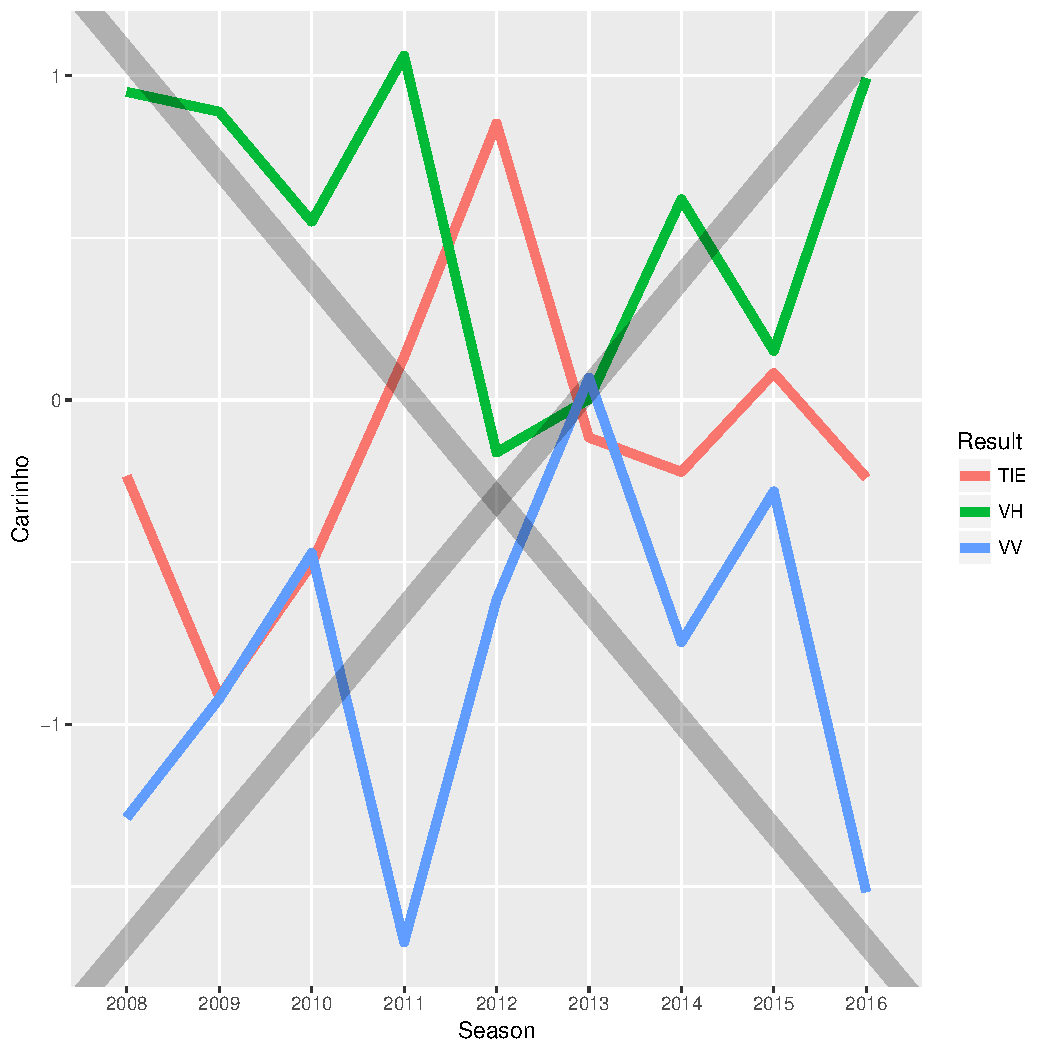
\includegraphics[width=25mm]{carrinho_result} &
  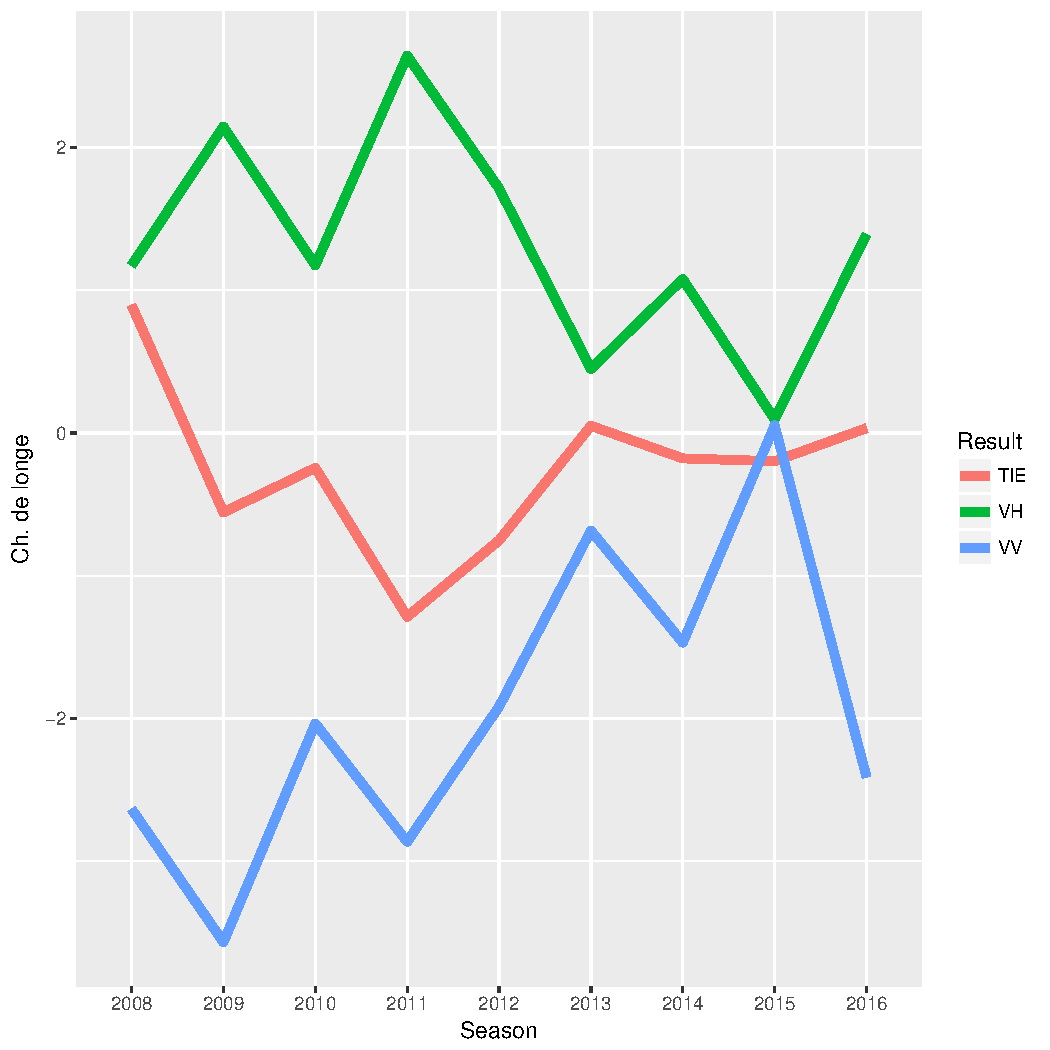
\includegraphics[width=25mm]{ch_delonge_result} \\
\scriptsize{(a) Aceleração } & \scriptsize{(b) altura  } & \scriptsize{(c) cabeceio } & \scriptsize{(d) carrinho } & \scriptsize{(e) chute de longe }\\[3pt]
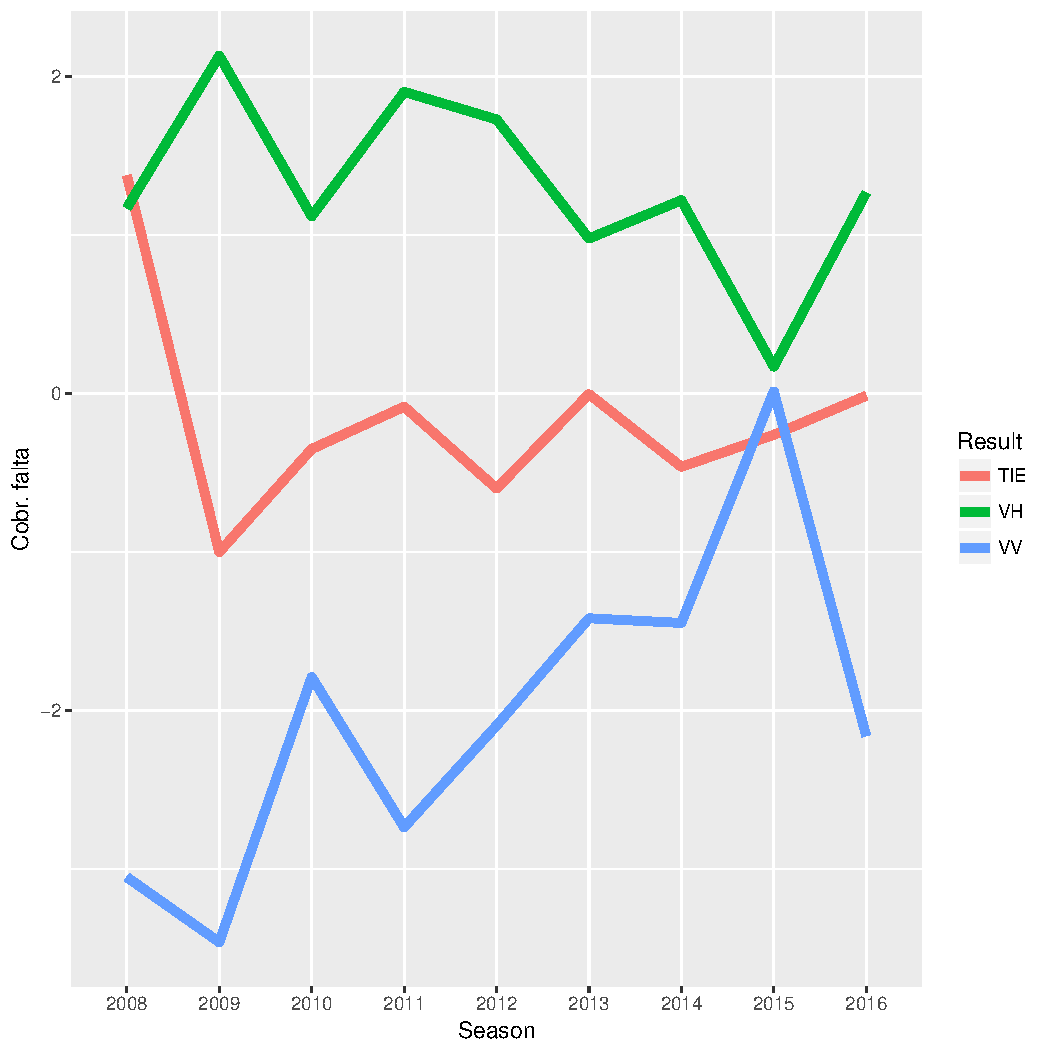
\includegraphics[width=25mm]{cobr_falta_result} & 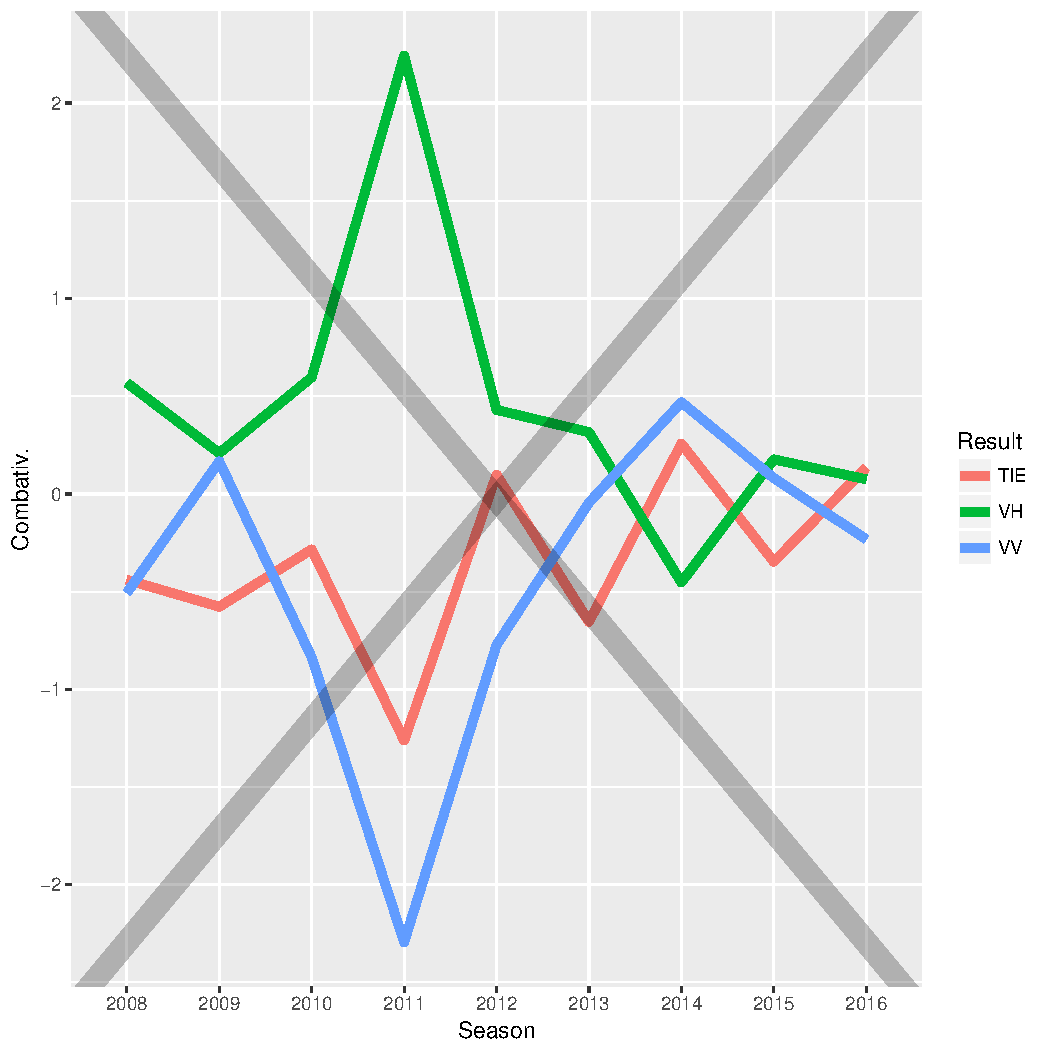
\includegraphics[width=25mm]{combativ__result} &   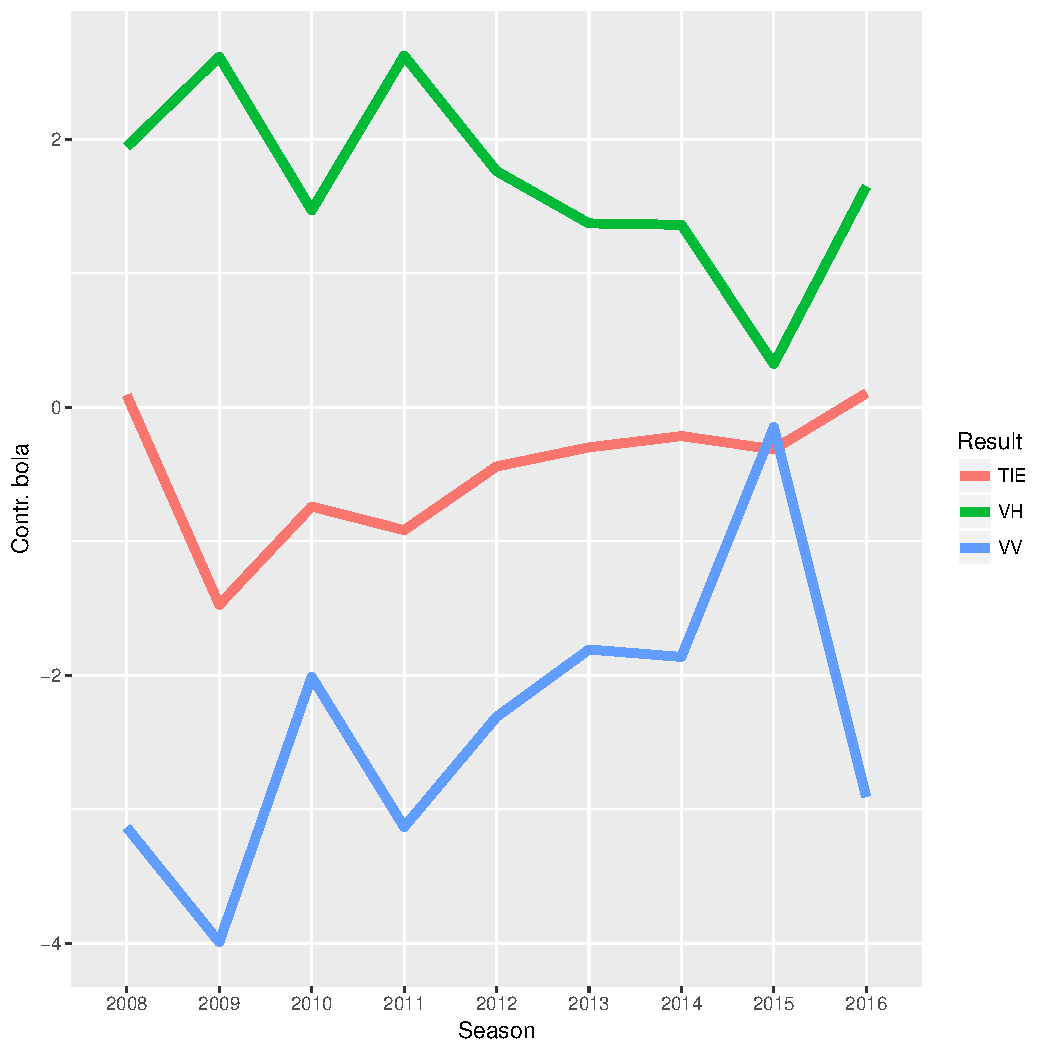
\includegraphics[width=25mm]{contr_bola_result} &
  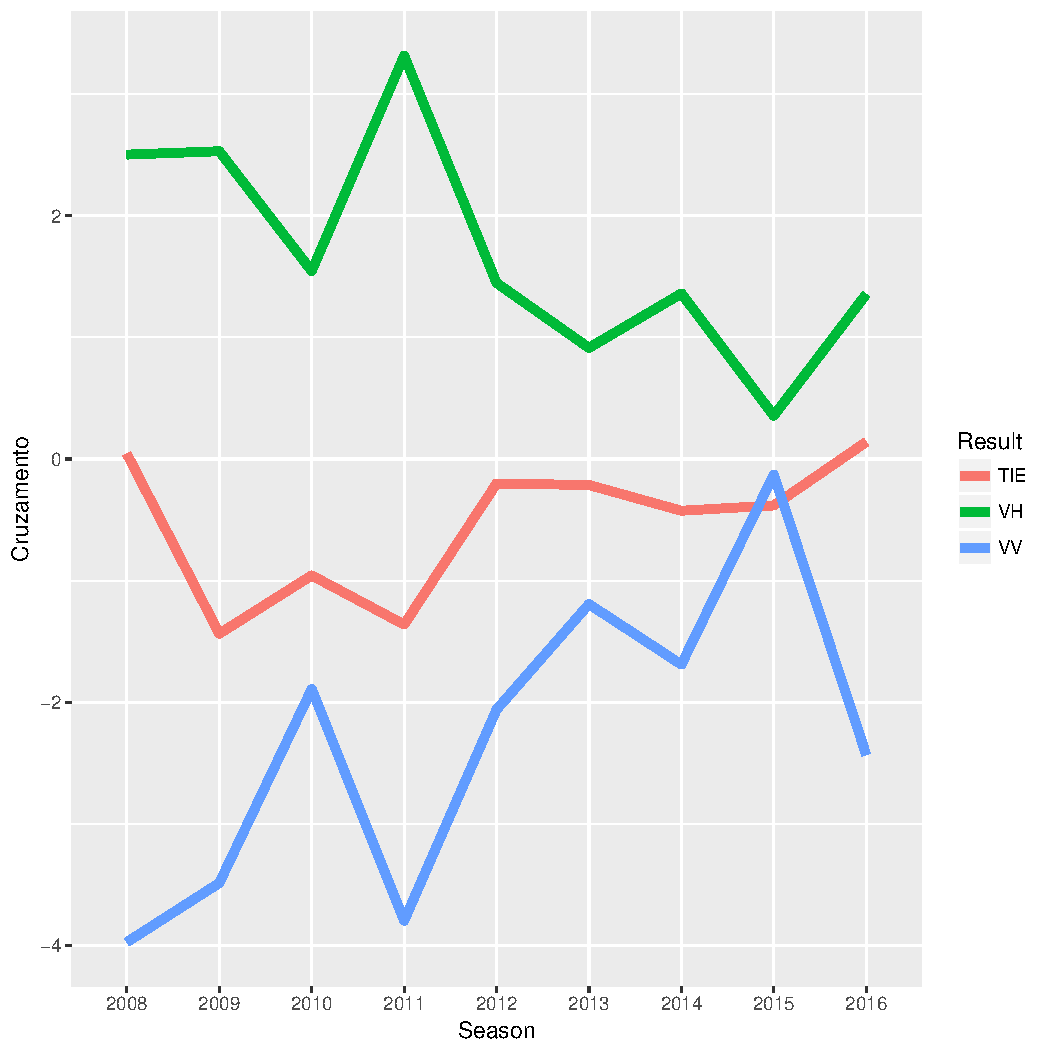
\includegraphics[width=25mm]{cruzamento_result} & 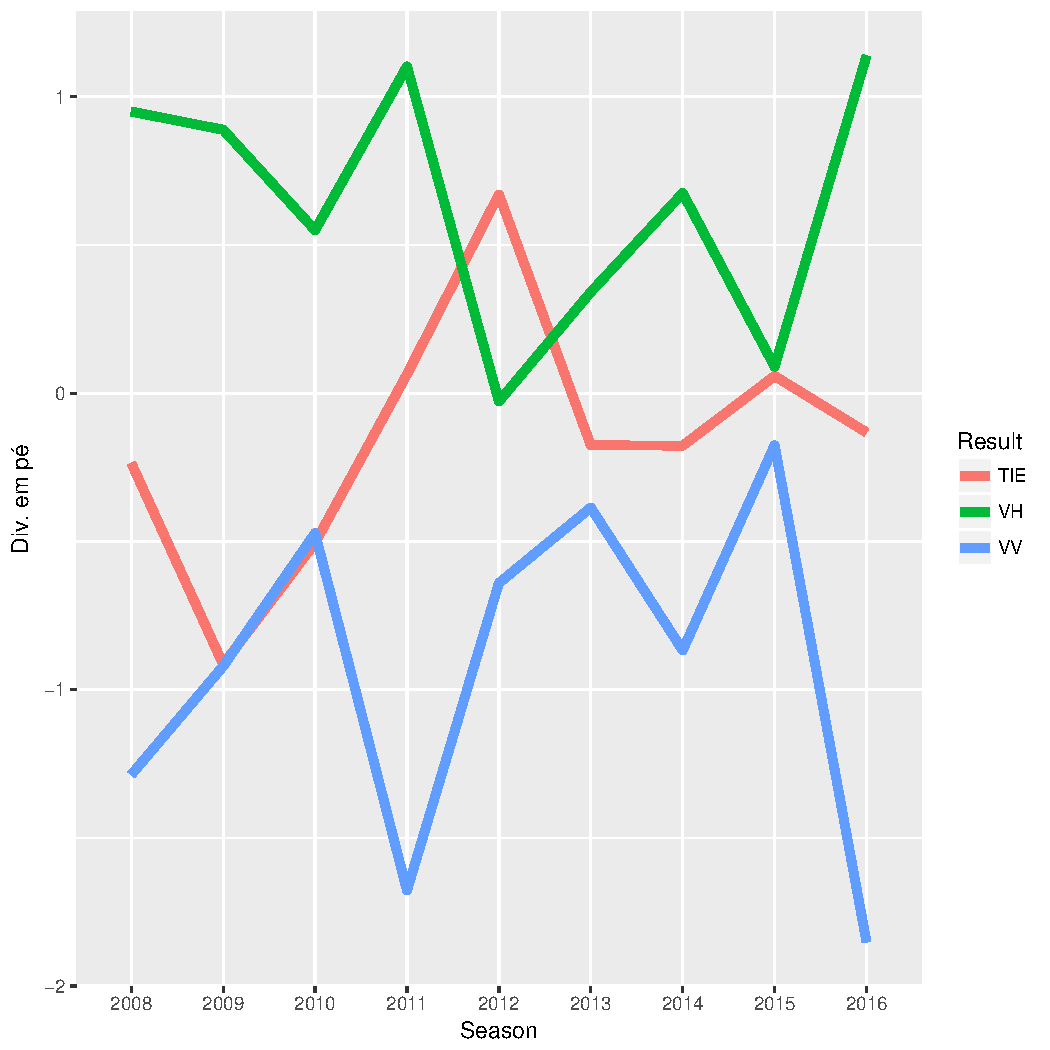
\includegraphics[width=25mm]{div_empe_result} \\
 \scriptsize{(f) cobrança de falta } & \scriptsize{(g) combatividade } & \scriptsize{(h) controle de bola} & \scriptsize{(i) cruzamento} & \scriptsize{(j) dividida}\\[3pt]
 
 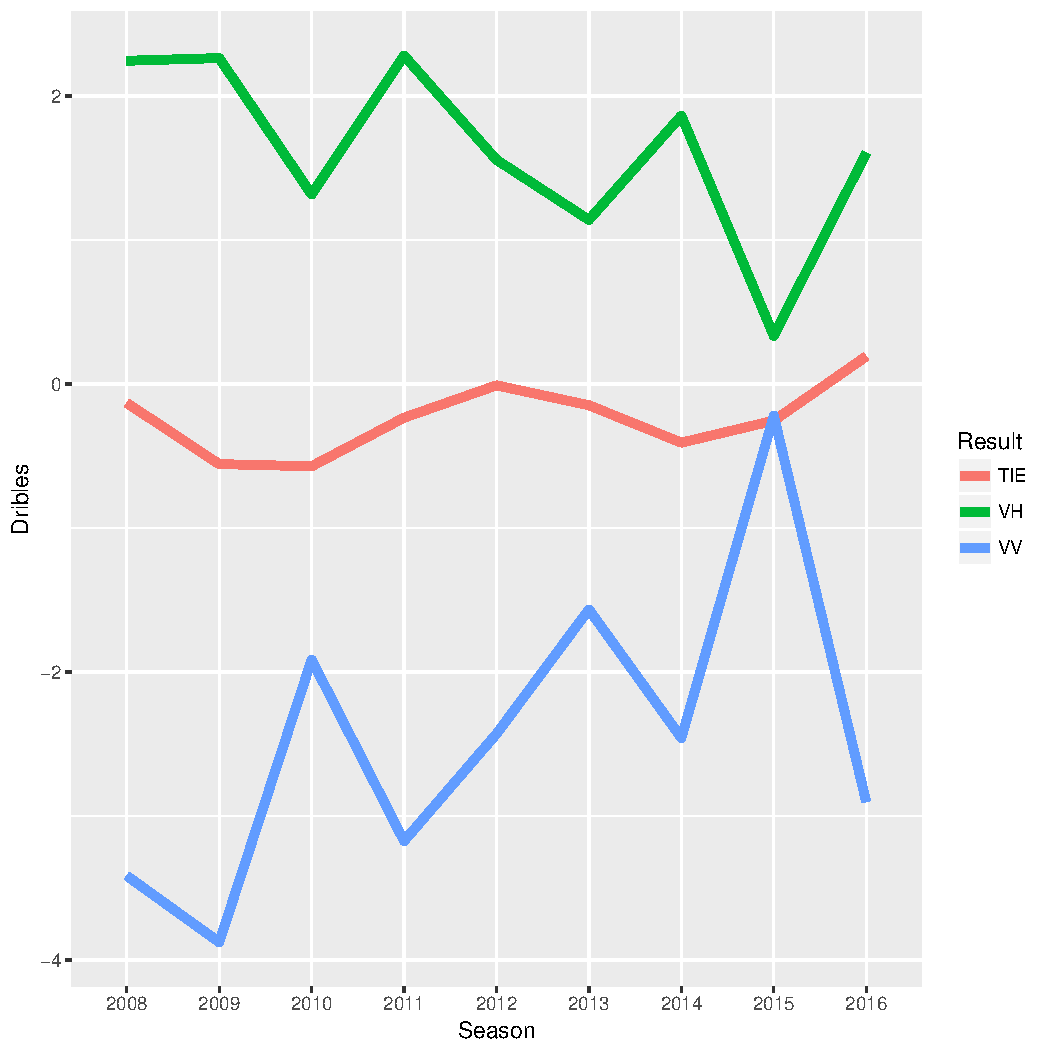
\includegraphics[width=25mm]{dribles_result} & 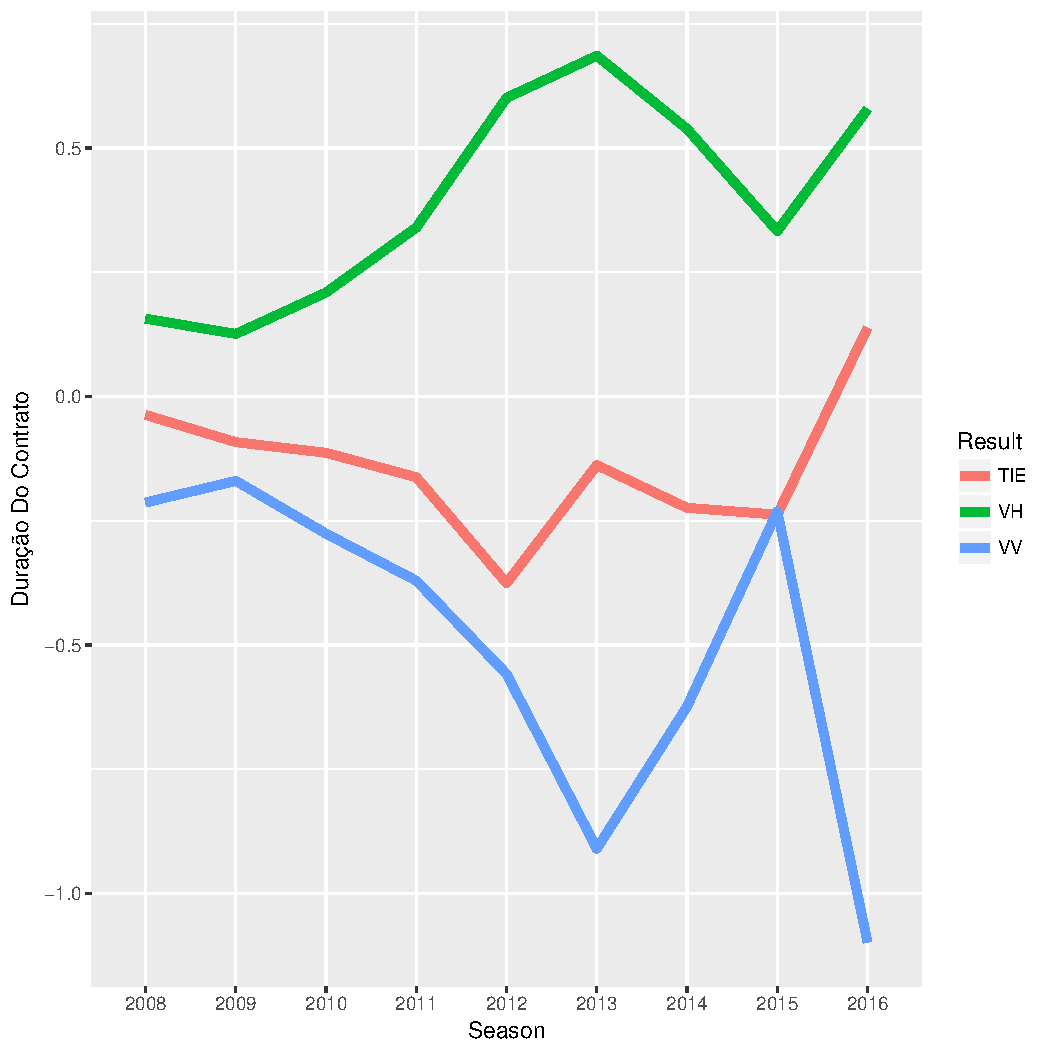
\includegraphics[width=25mm]{duracaodocontrato_result} &   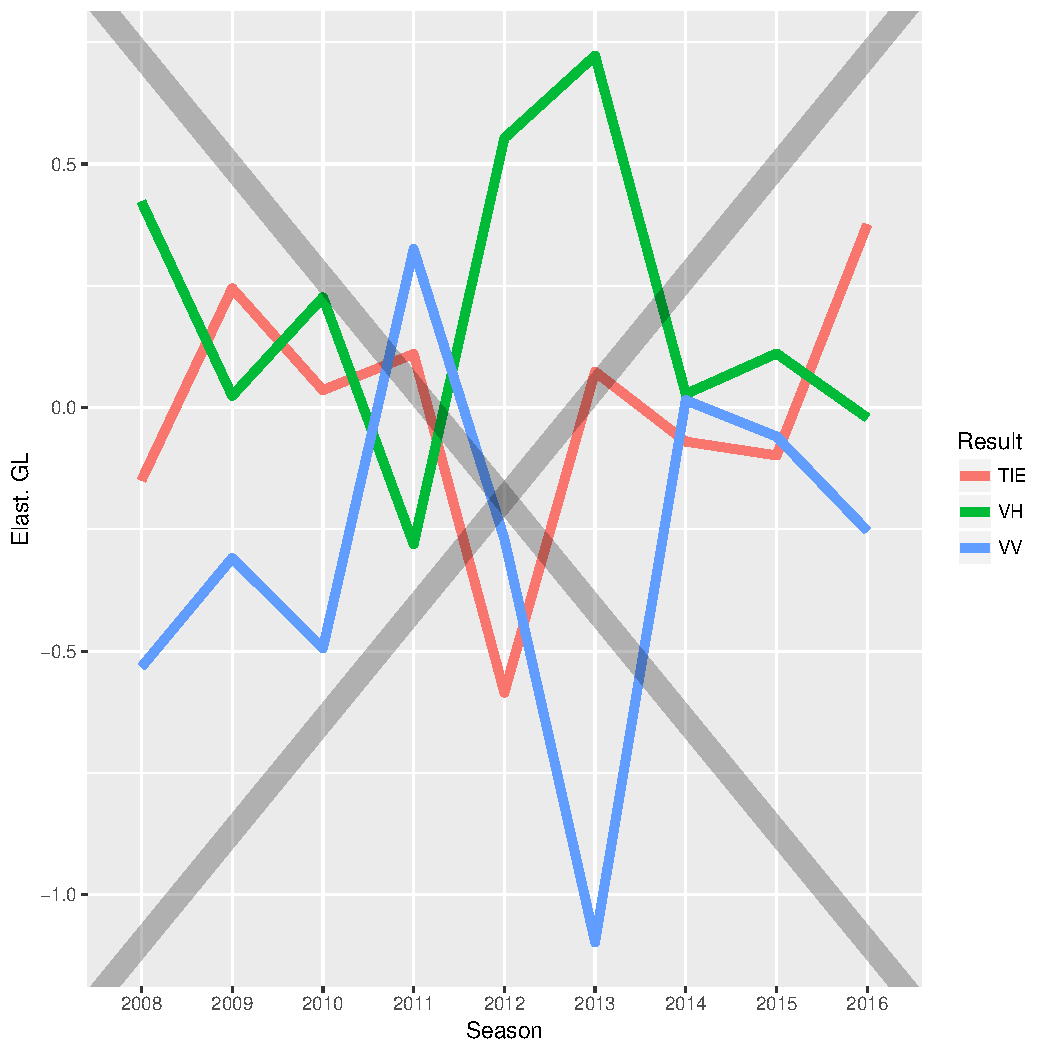
\includegraphics[width=25mm]{elast_gl_result} &
  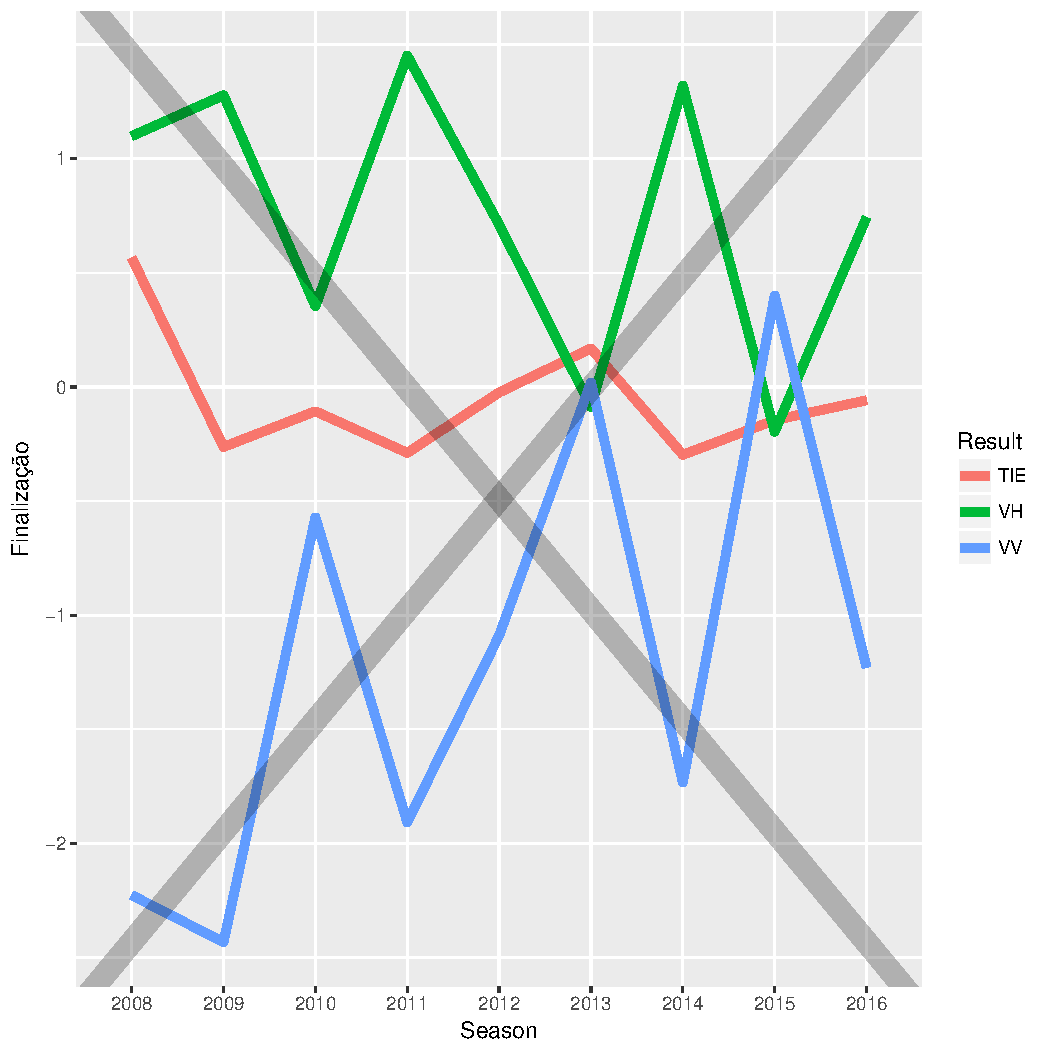
\includegraphics[width=25mm]{finalizacao_result} & 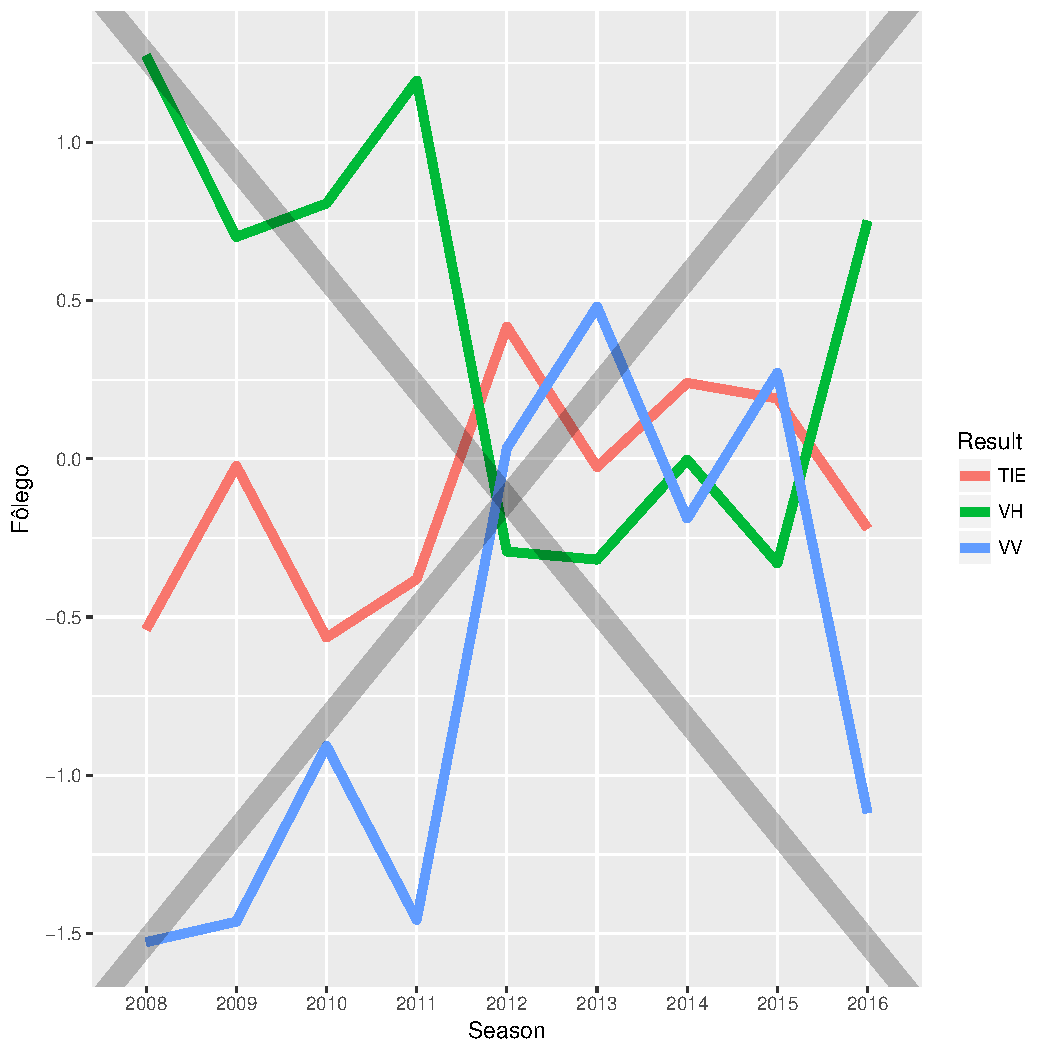
\includegraphics[width=25mm]{folego_result}  \\
 \scriptsize{(k) drible} & \scriptsize{(l) duração do contrato } & \scriptsize{(m) elasticidade do goleiro} & \scriptsize{(n) finalização} & \scriptsize{(o) fôlego}\\[3pt]
 
  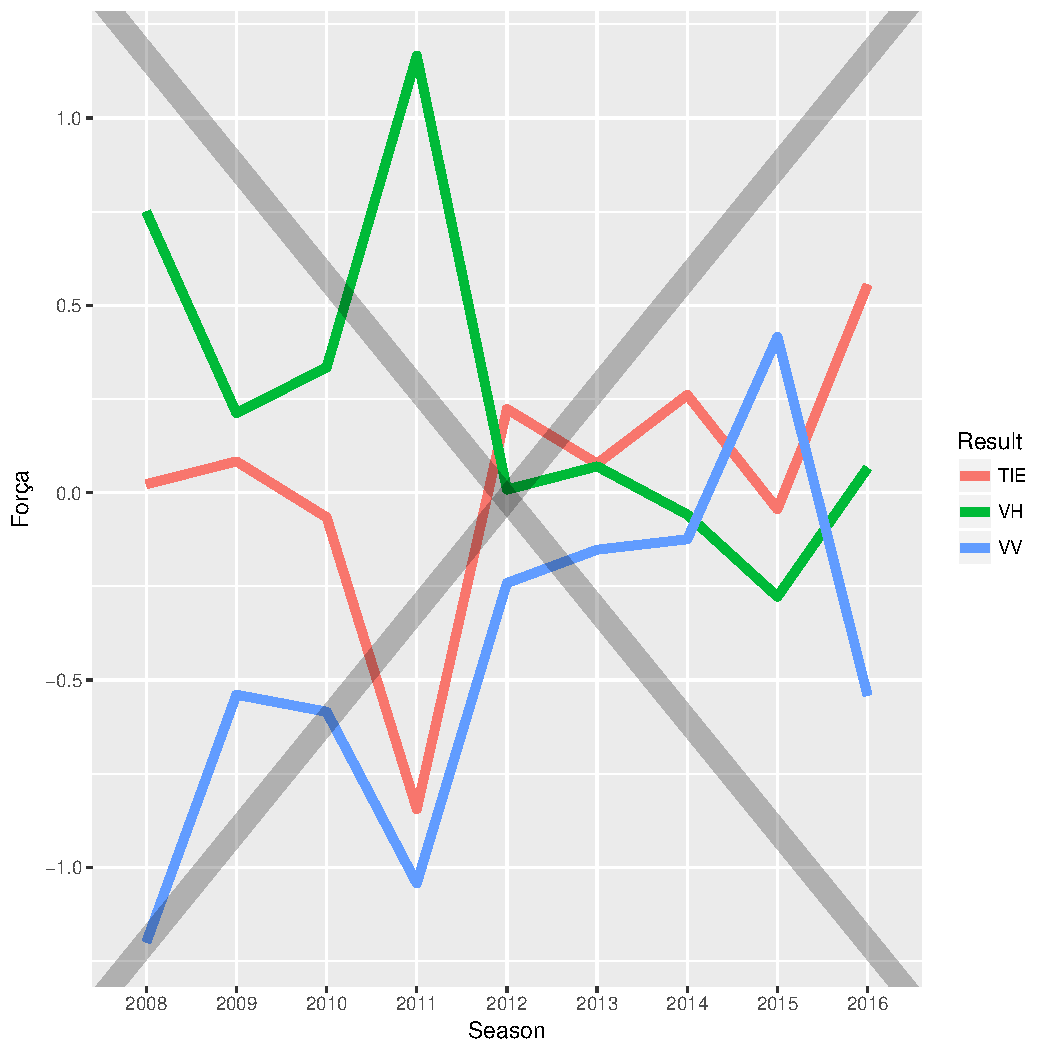
\includegraphics[width=25mm]{forca_result} & 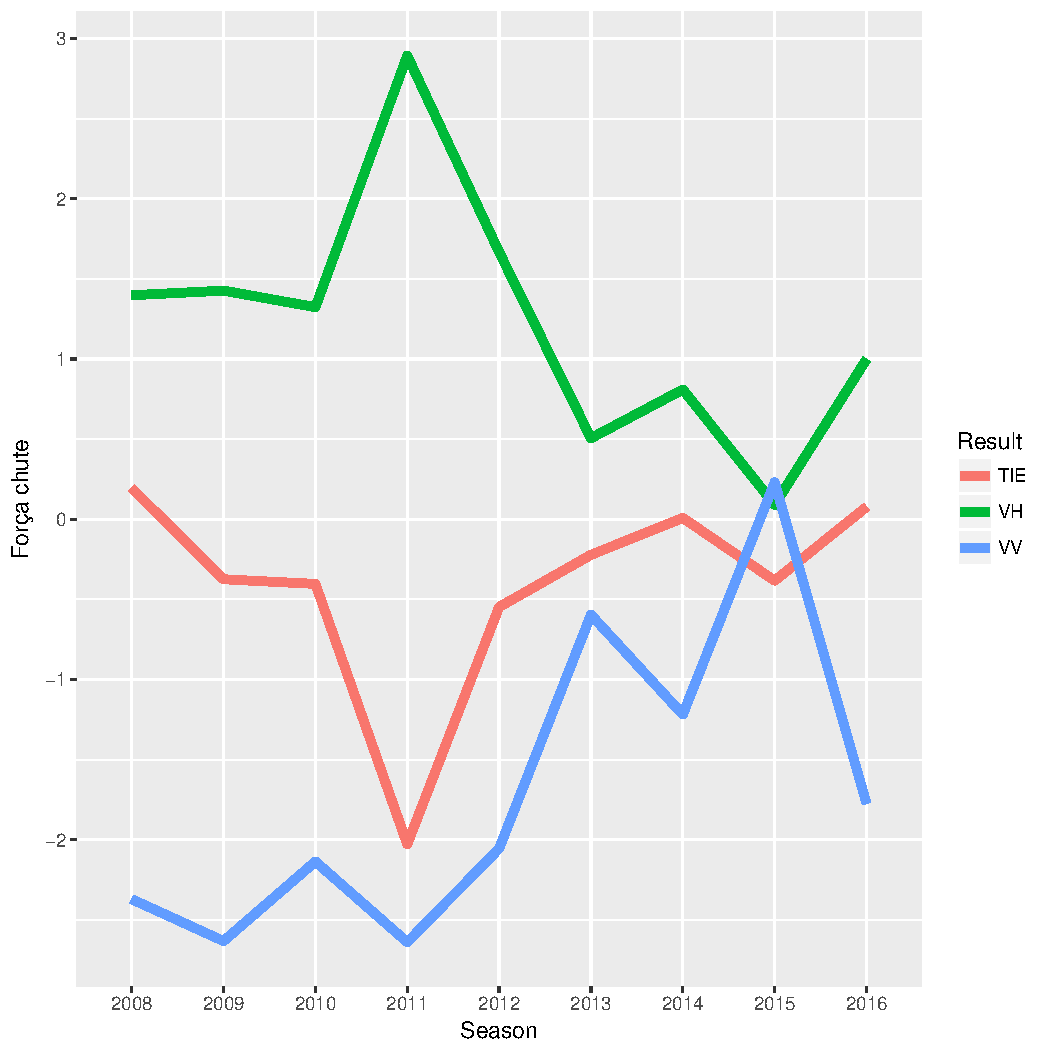
\includegraphics[width=25mm]{forcachute_result}  &   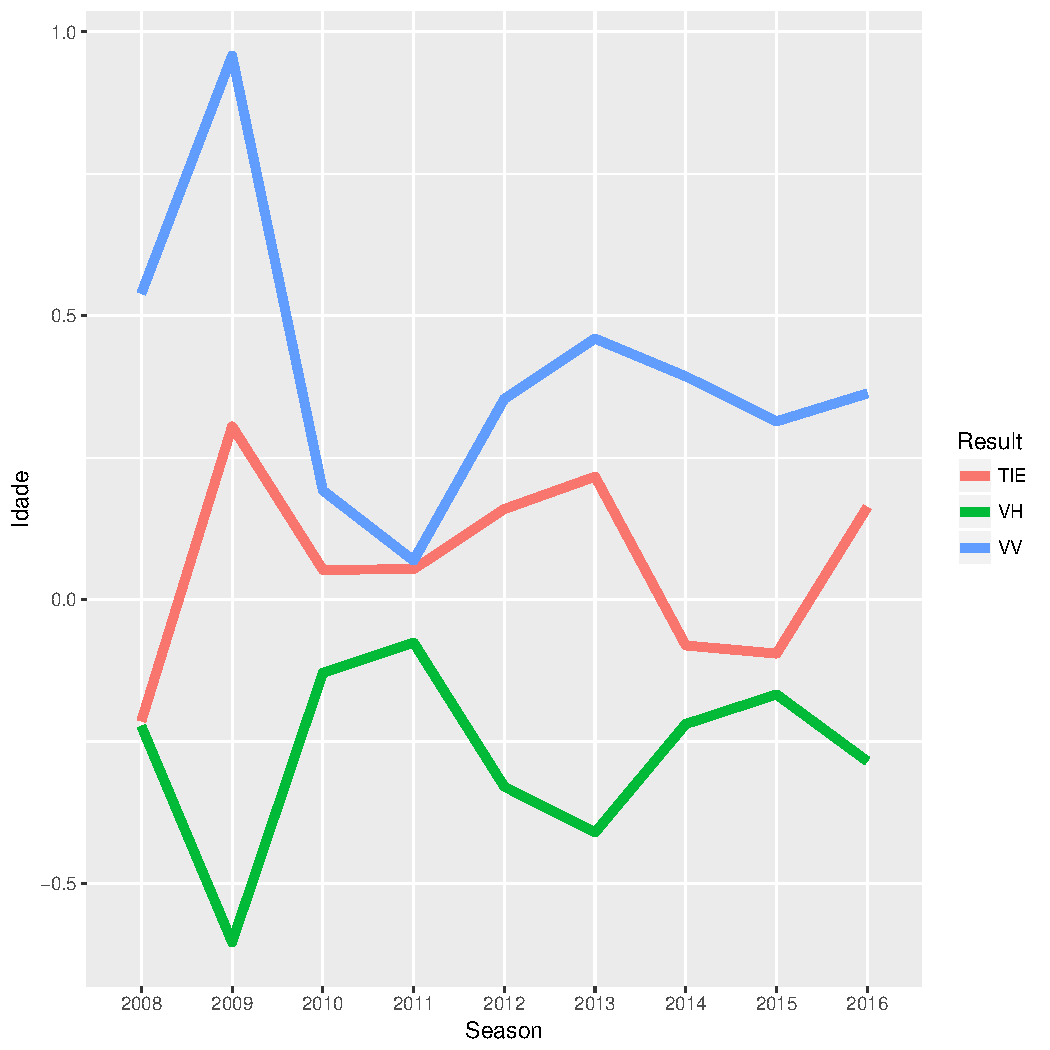
\includegraphics[width=25mm]{idade_result} &
  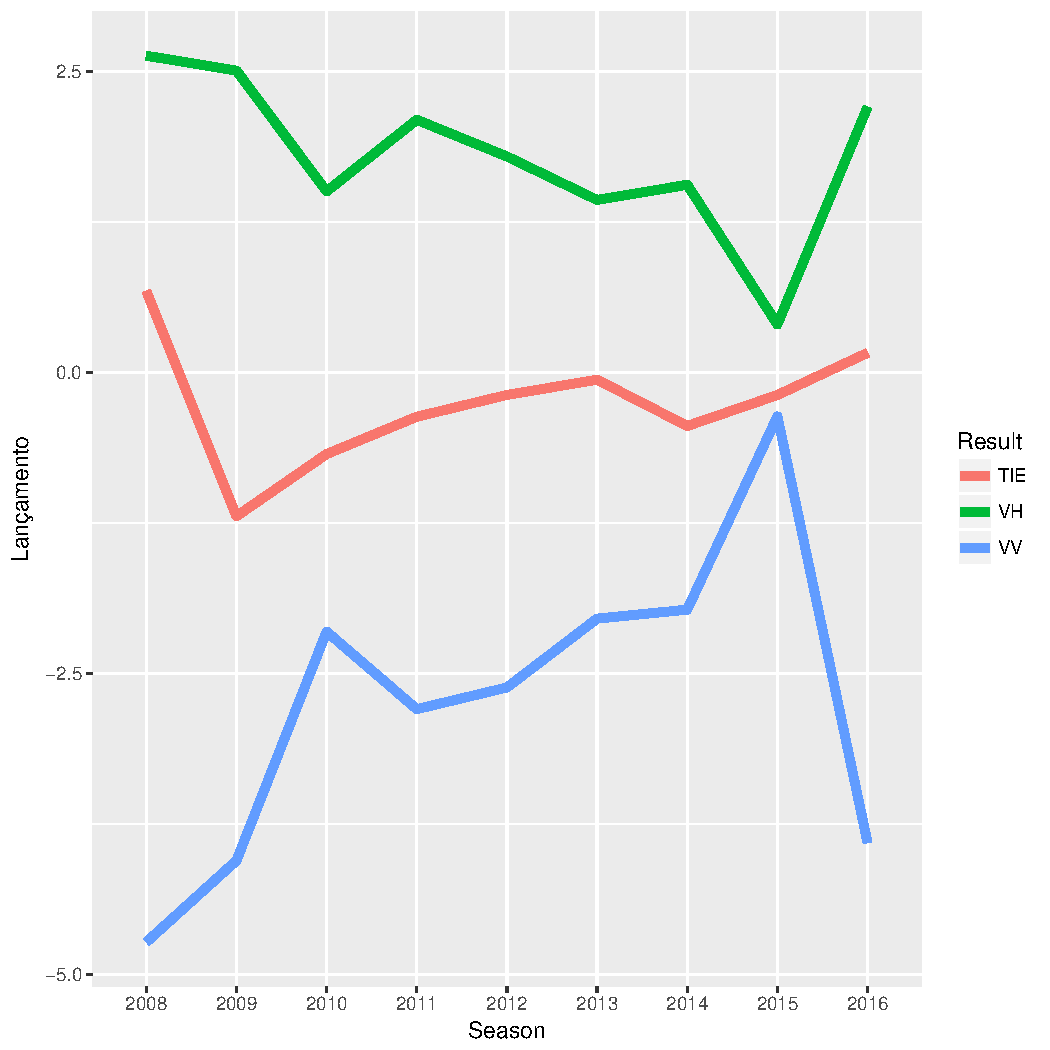
\includegraphics[width=25mm]{lancamento_result}  & 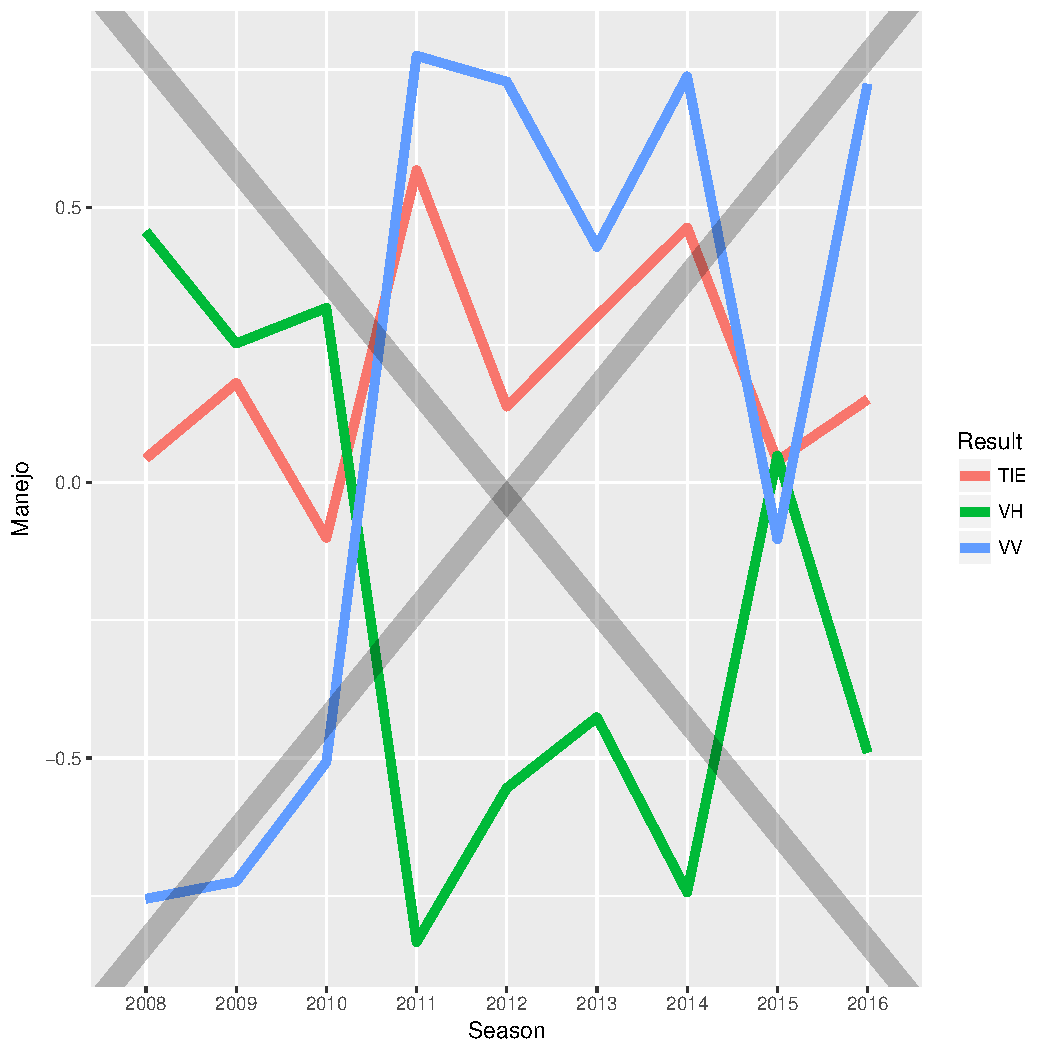
\includegraphics[width=25mm]{manejo_result}  \\
 \scriptsize{(p) força} & \scriptsize{(q) força chute } & \scriptsize{(r) idade} & \scriptsize{(s) lançamento} & \scriptsize{(t) manejo}\\[3pt]
 
   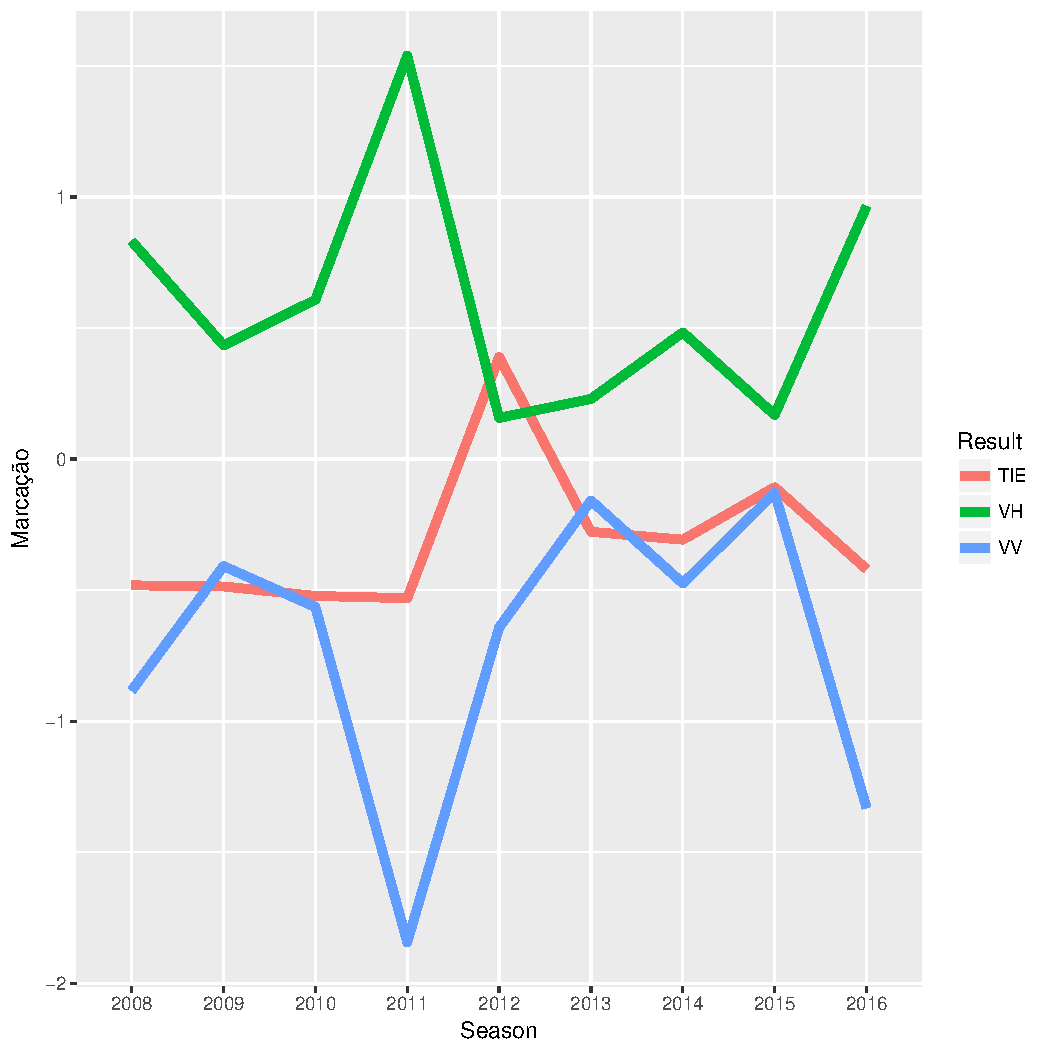
\includegraphics[width=25mm]{marcacao_result} & 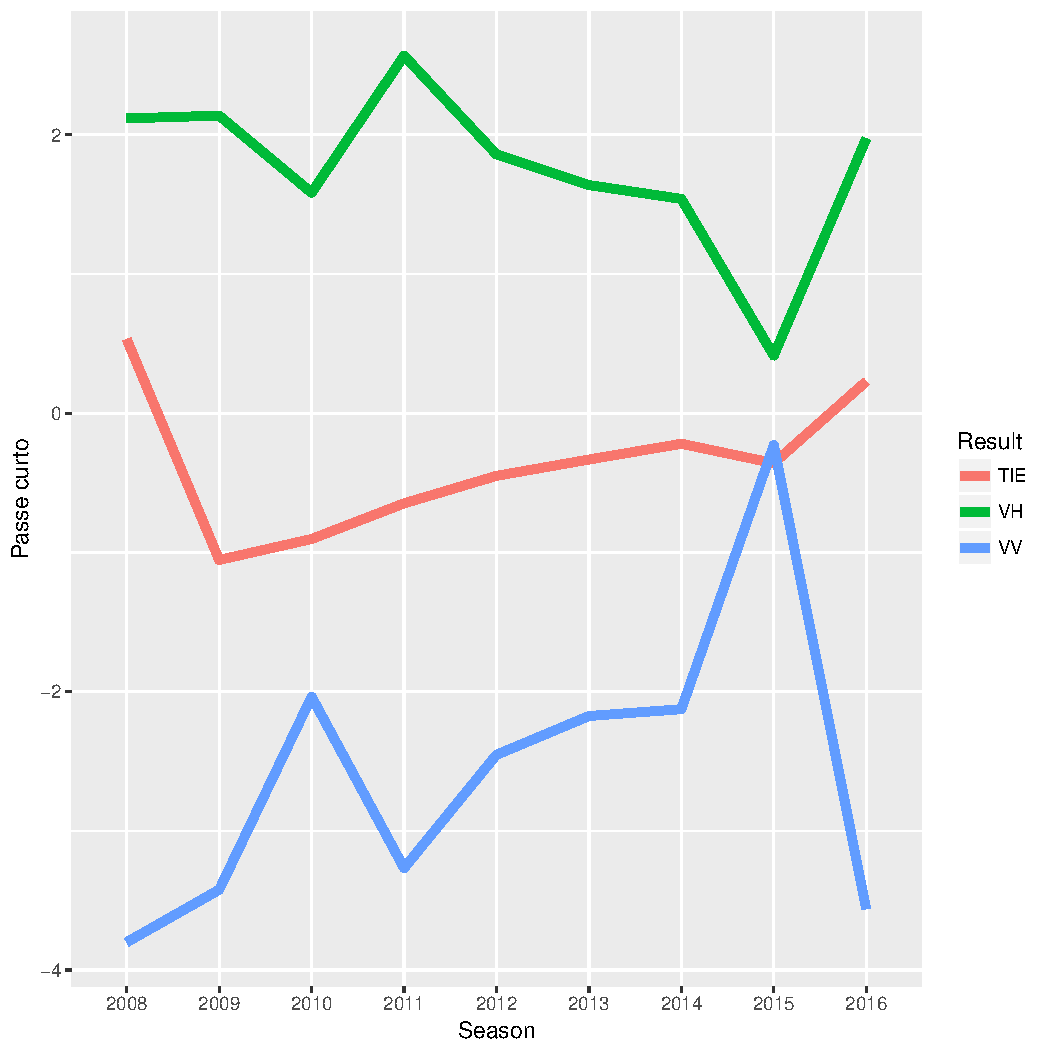
\includegraphics[width=25mm]{passecurto_result}   &   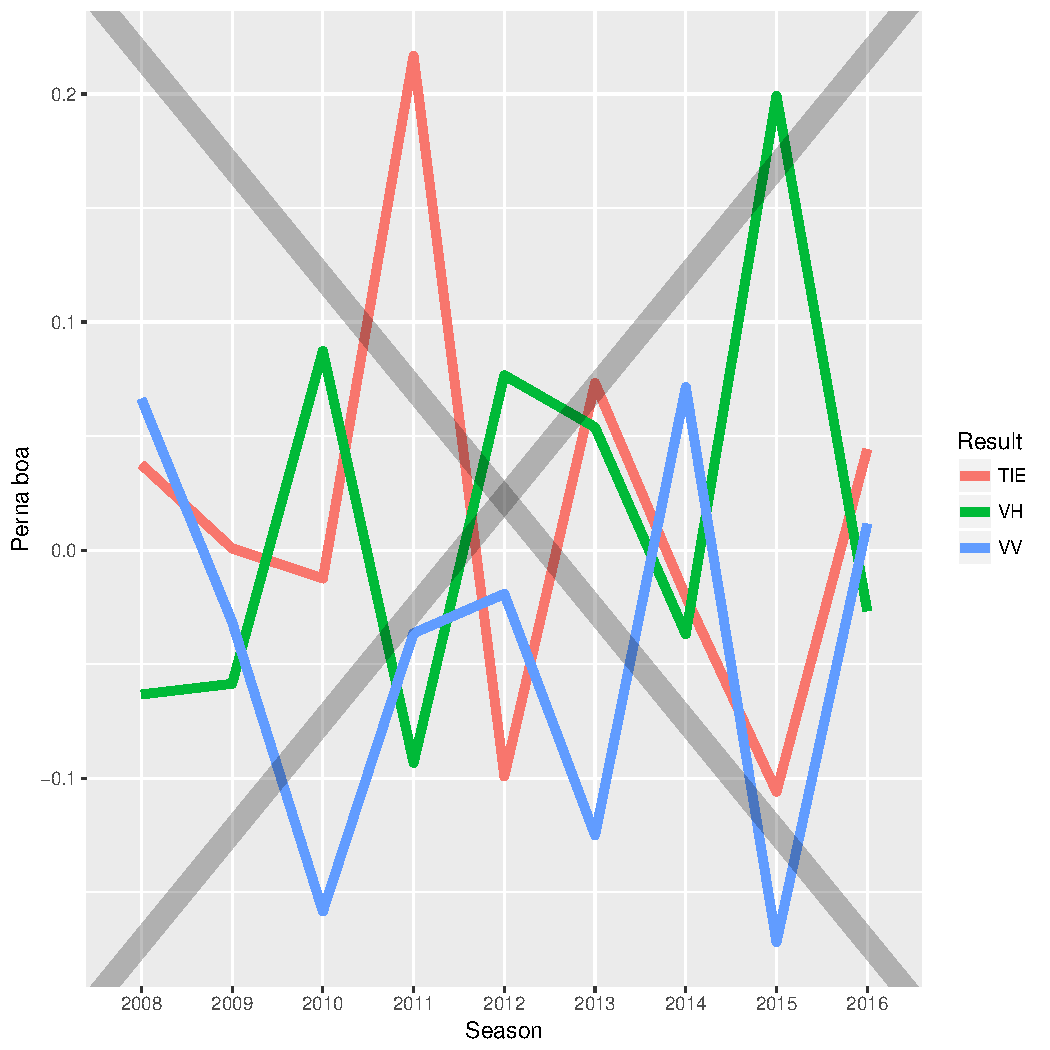
\includegraphics[width=25mm]{pernaboa_result}&
  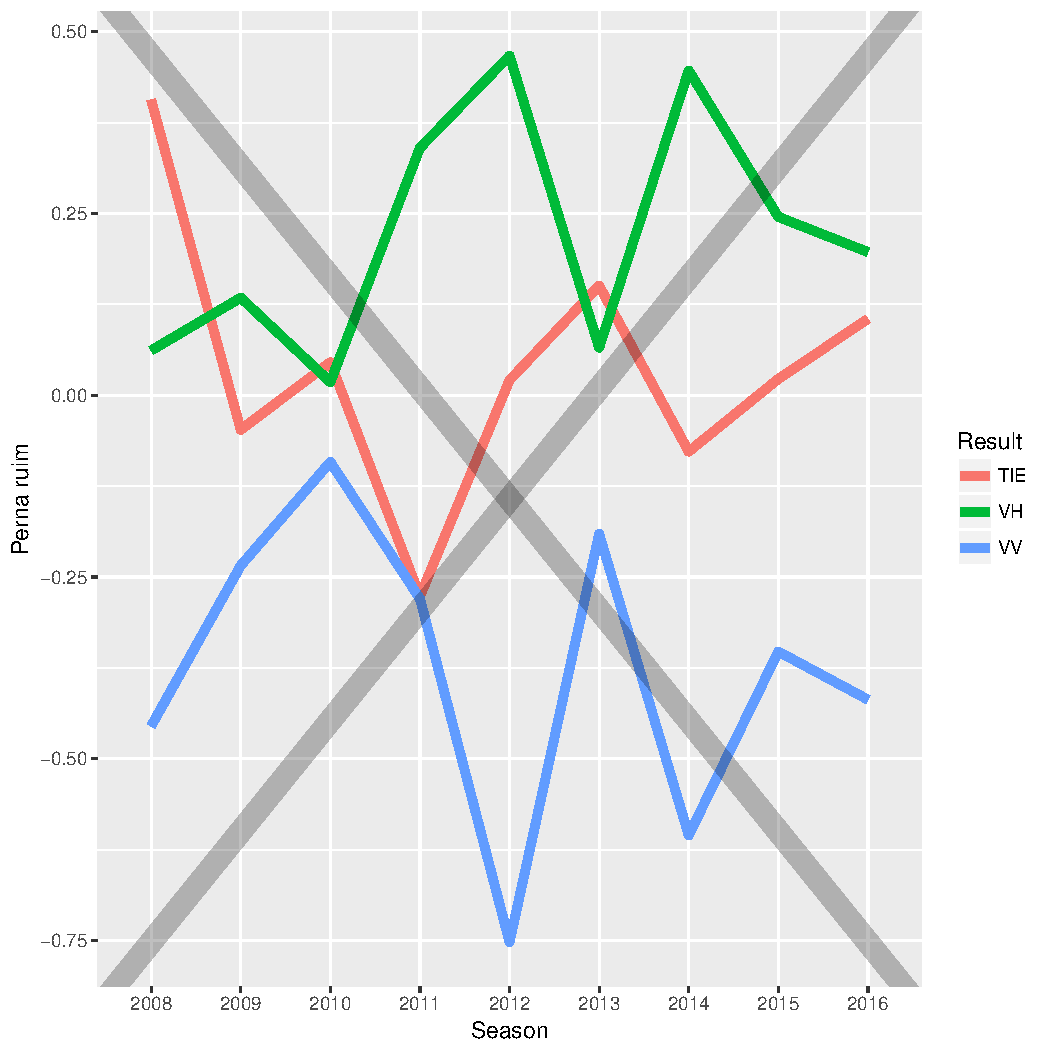
\includegraphics[width=25mm]{pernaruim_result}   & 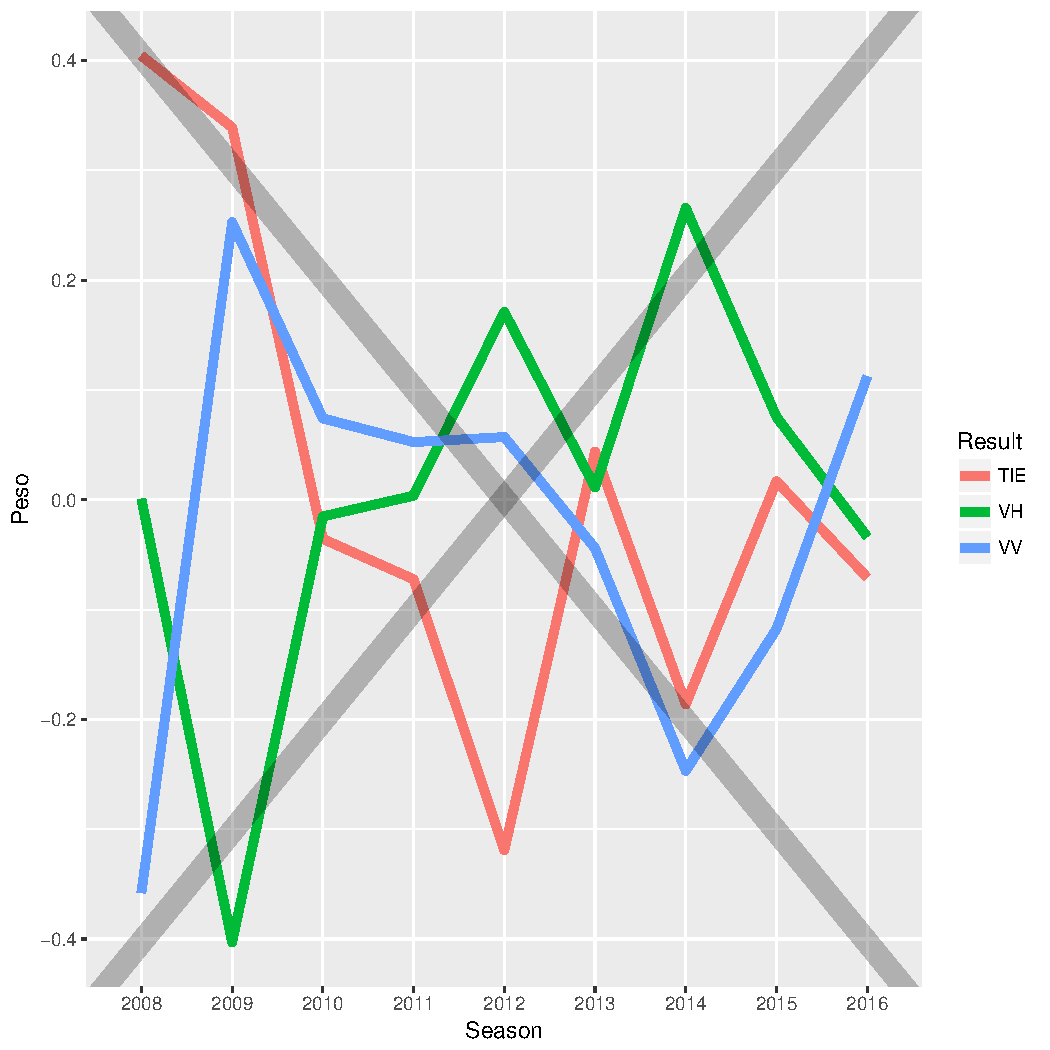
\includegraphics[width=25mm]{peso_result}   \\
 \scriptsize{(u) marcação} & \scriptsize{(v) passe curto } & \scriptsize{(w) perna boa} & \scriptsize{(x) perna ruim} & \scriptsize{(y) peso}\\[3pt]
 
    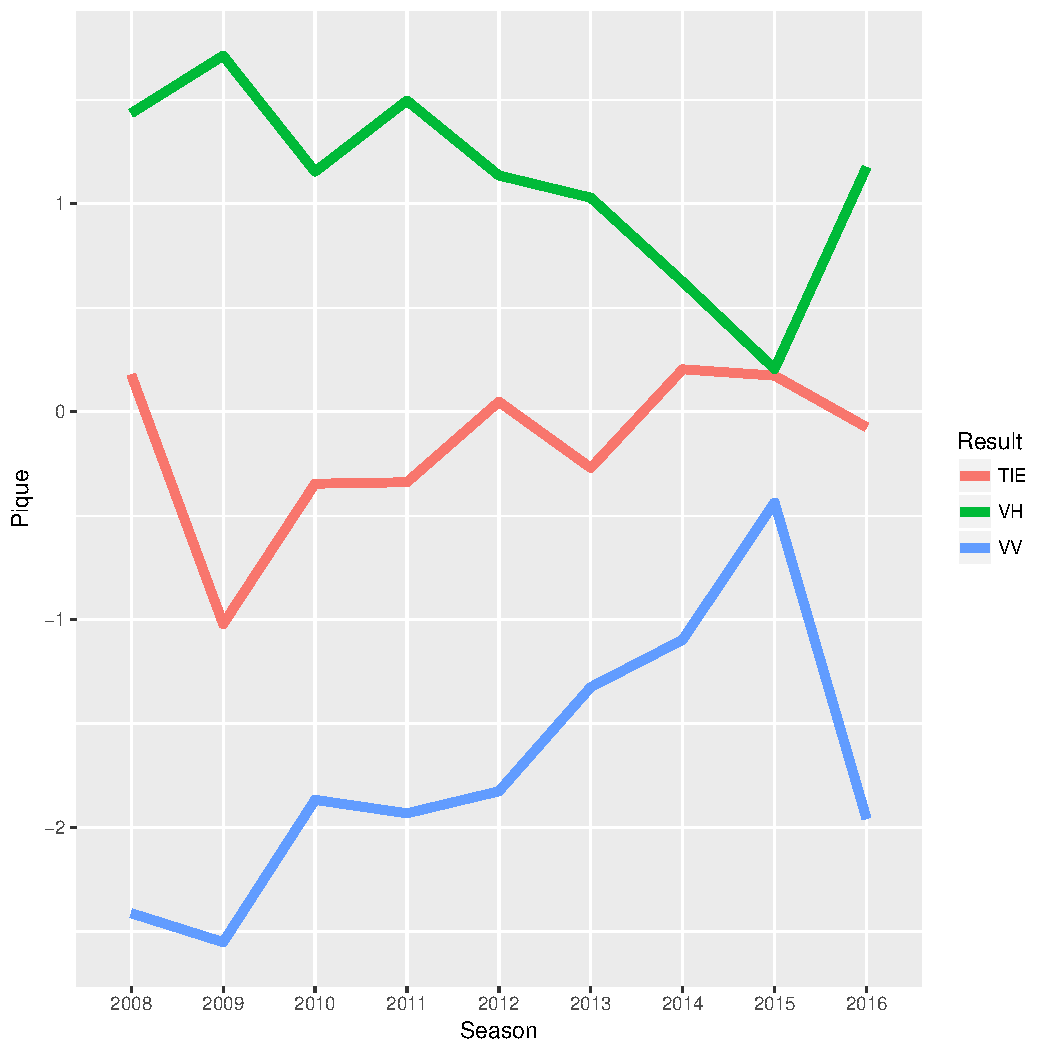
\includegraphics[width=25mm]{pique_result}  & \includegraphics[width=25mm]{pos_result} & 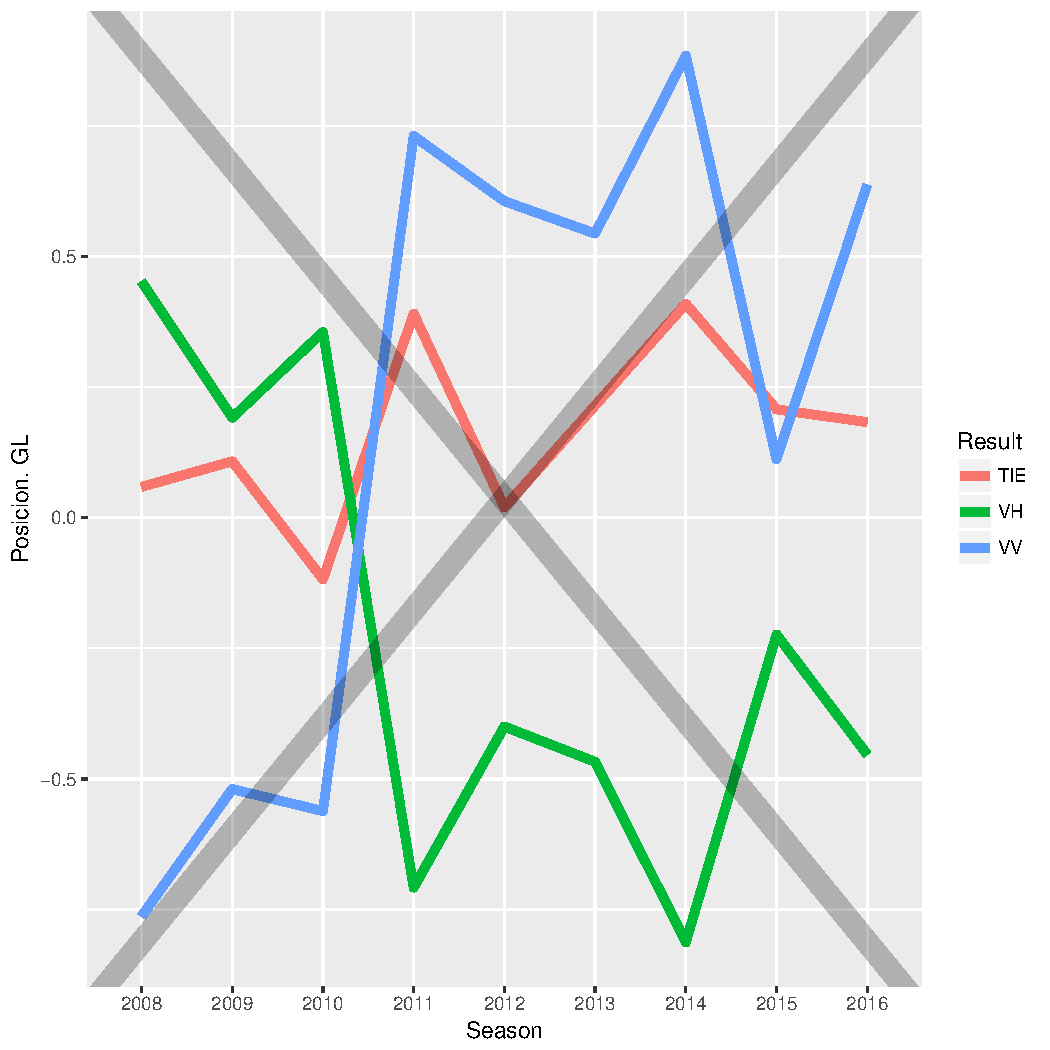
\includegraphics[width=25mm]{posicion_gl_result} &     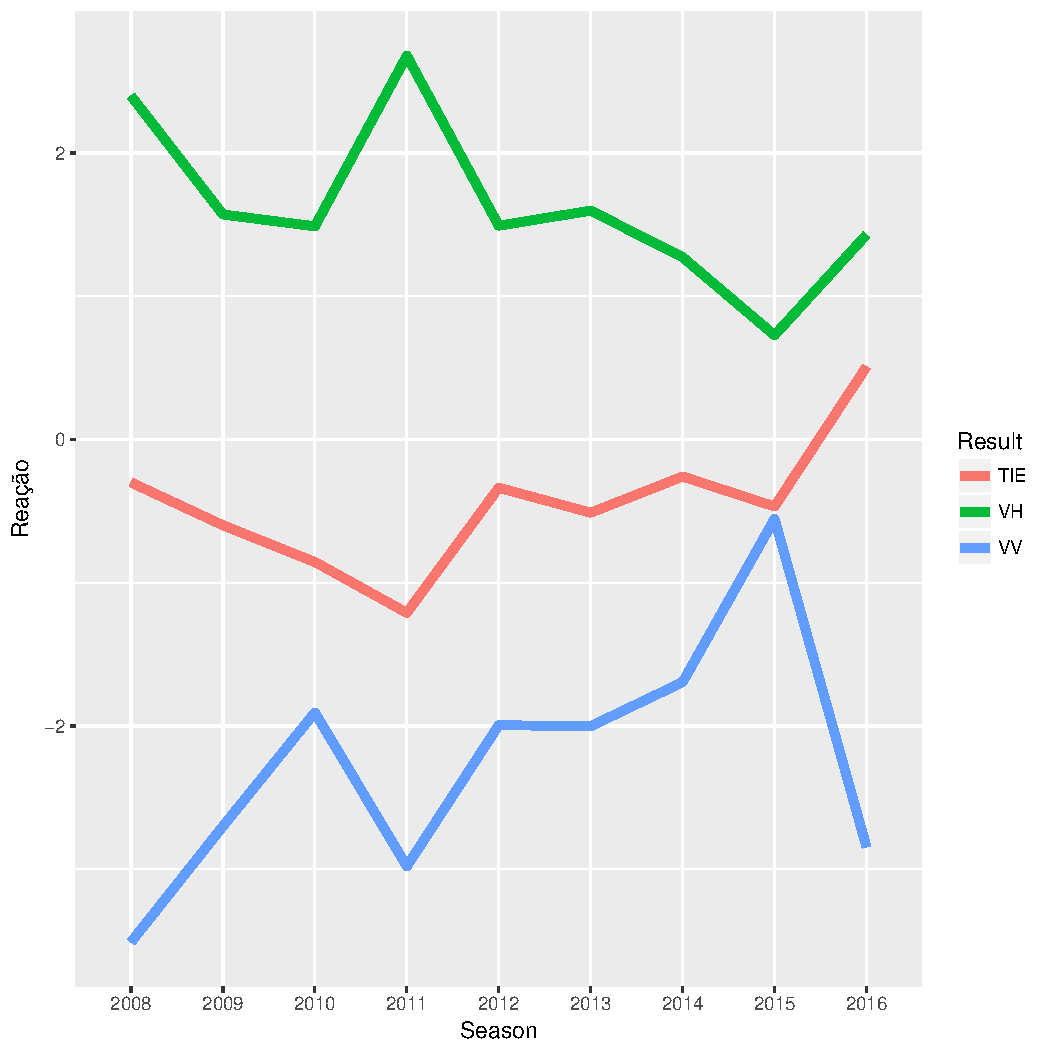
\includegraphics[width=25mm]{reacao_result}&
  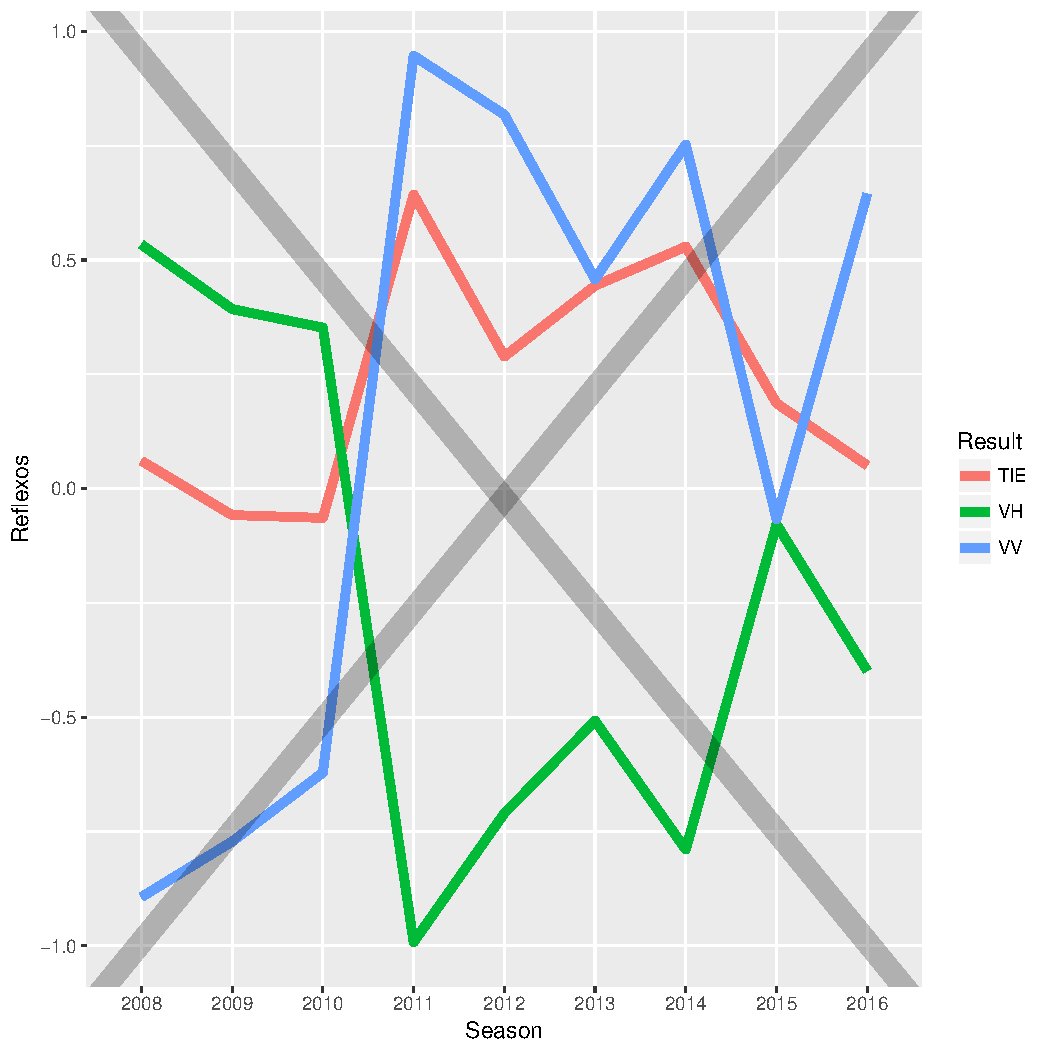
\includegraphics[width=25mm]{reflexos_result}     \\
 \scriptsize{(z) pique} & \scriptsize{(aa) posição}& \scriptsize{(ab) posição do goleiro} & \scriptsize{(ac) reação} & \scriptsize{(ad) reflexo}  \\[3pt]

\end{tabular}
    \caption[\scriptsize{Medidas resumo.}]{\scriptsize{Medidas resumo ao longo das temporadas para cada variável disponível. O marcador $X$ é inserido para os gráficos das variáveis não utilizadas para o modelo, por apresentar inconsistências nas relações positivas e negativas.}}
        \label{fig:medresumo}
\end{figure}


Com esse critério são selecionadas as variáveis Aceleração, Ch. de longe, Cobr. falta, Contr. bola, Cruzamento, Div. em pé, Dribles, Duração Do Contrato, Força chute, Idade, Lançamento, Marcação, Passe curto, Pique, Posição e Reação.

O segundo critério seleciona as variáveis para modelar o empate do time mandante. A partir da tabela \ref{tab:selectvartrans} foram selecionados aqueles que possuem a variável MNP com valor superior ou igual a $1$, isso é, variáveis as quais a transformação \ref{eq:transform} resulta em uma alta similaridade nas habilidades dos times que empataram e baixa similaridade dos resultados que não ocorreram empate.



A figura \ref{fig:medresumo} destaca as variáveis selecionadas. Visualmente, esse filtro é realizado nos gráficos que possuem trajetórias em verde, empate, próxima de $1$ (alta similaridade) e sempre superiores às trajetorias de vitória e derrota do mandante, estando esses próximos de $0$ (baixa similaridade).

\begin{figure}
\begin{tabular}{ccccc}
  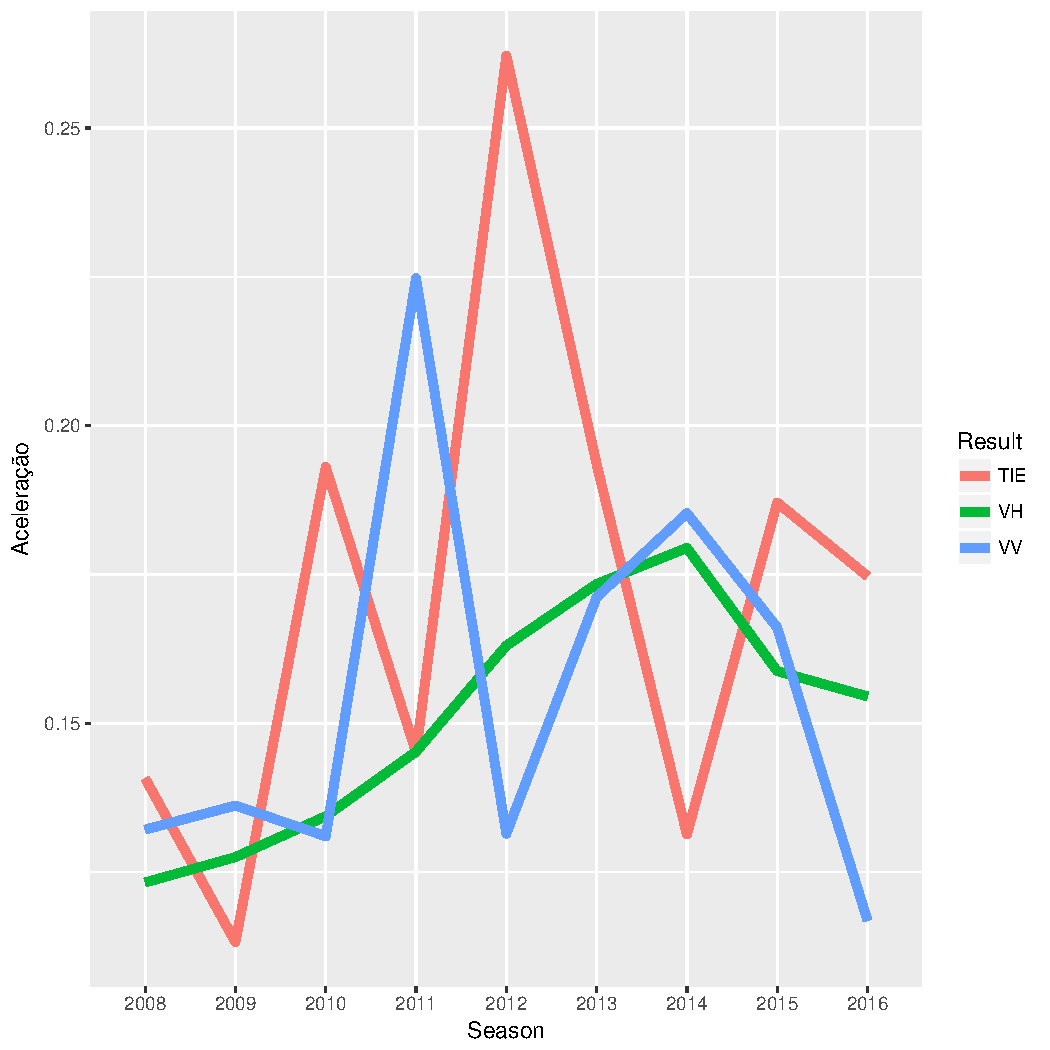
\includegraphics[width=25mm]{aceleracao_result_trans} & 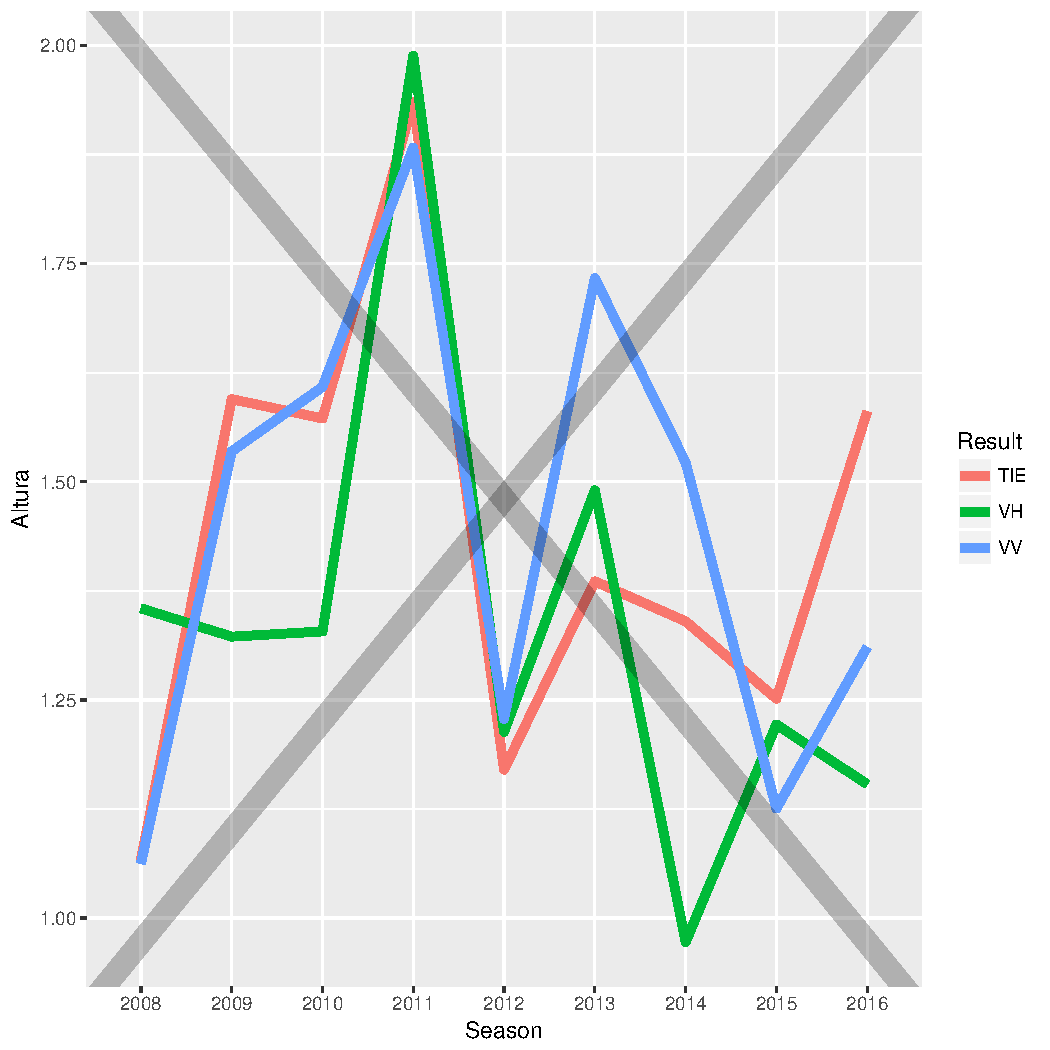
\includegraphics[width=25mm]{altura_result_trans} & 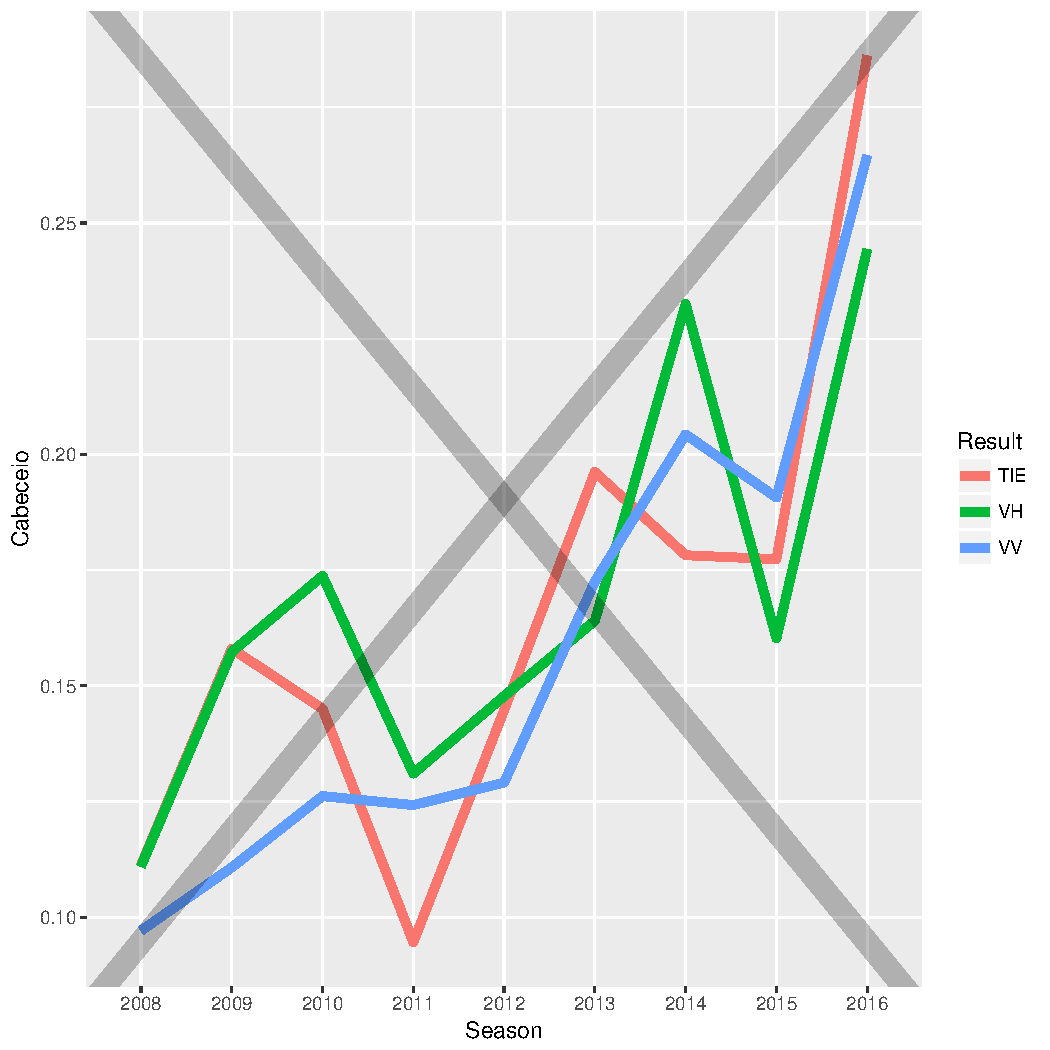
\includegraphics[width=25mm]{cabeceio_result_trans} &   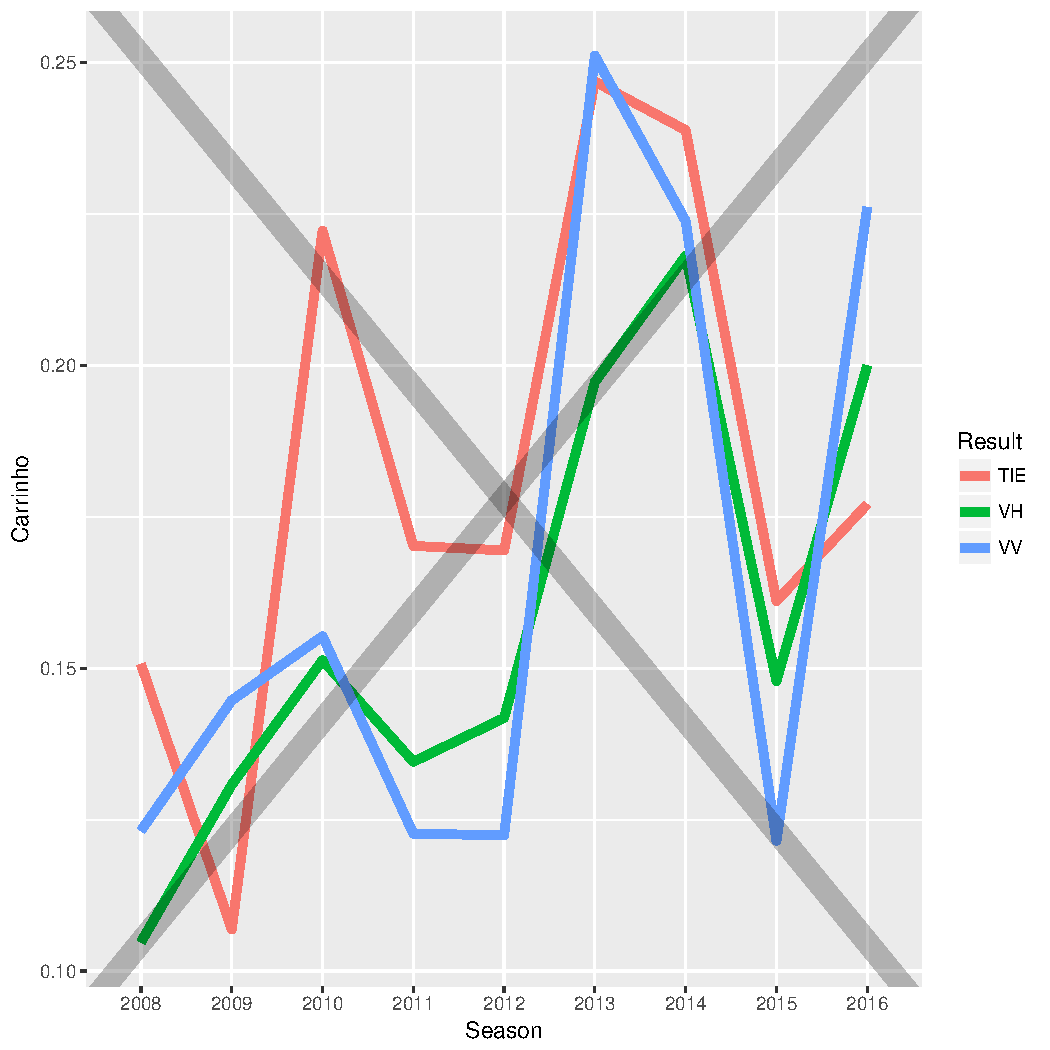
\includegraphics[width=25mm]{carrinho_result_trans} &
  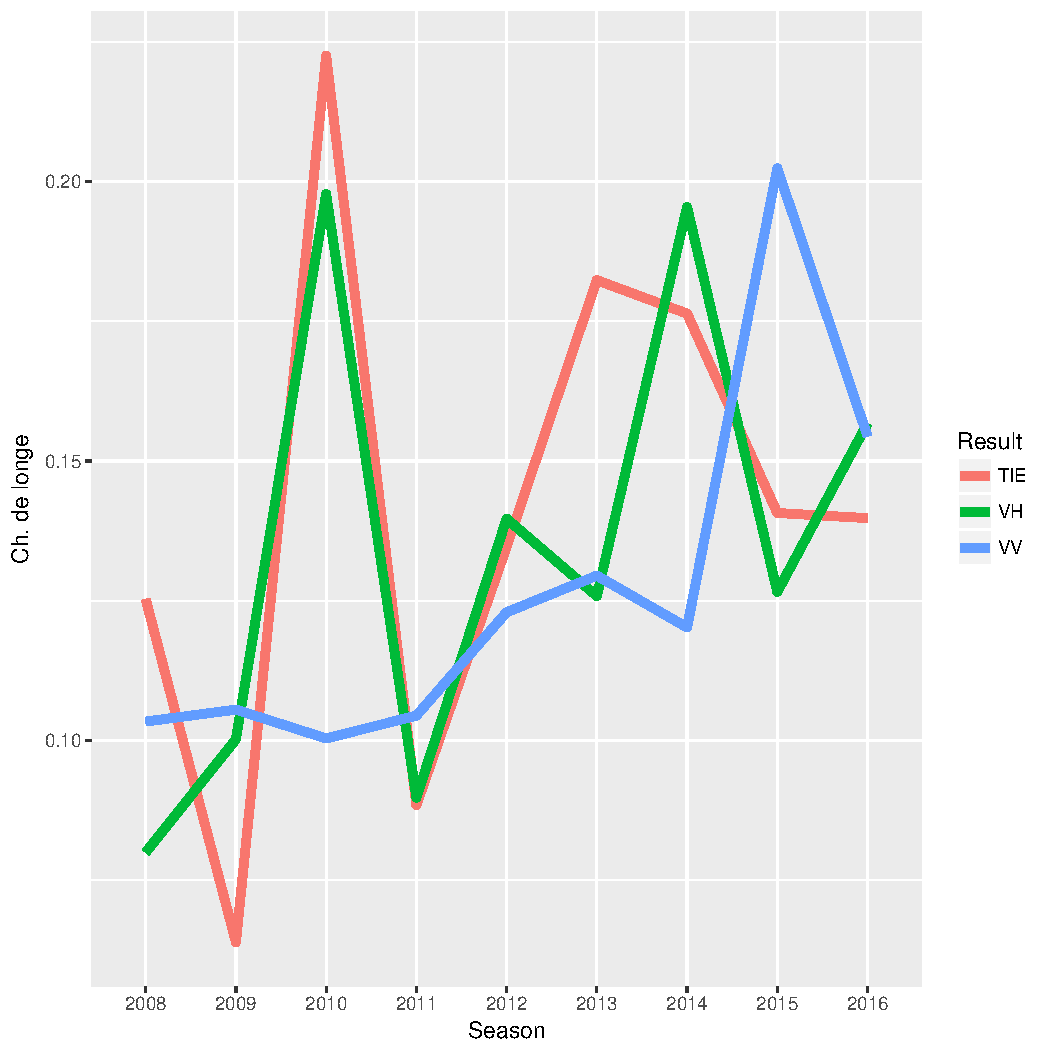
\includegraphics[width=25mm]{ch_delonge_result_trans} \\
\scriptsize{(a) Aceleração } & \scriptsize{(b) altura  } & \scriptsize{(c) cabeceio } & \scriptsize{(d) carrinho } & \scriptsize{(e) chute de longe }\\[3pt]
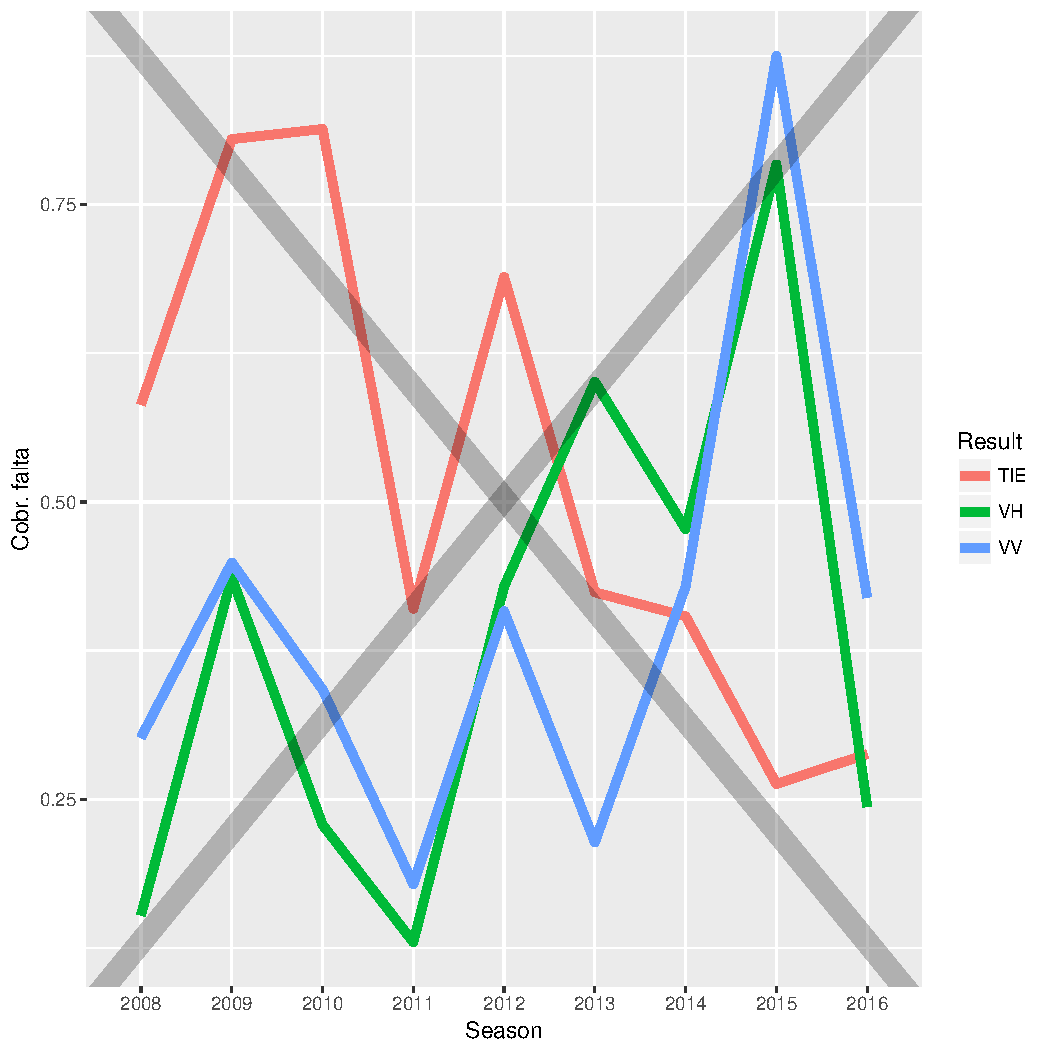
\includegraphics[width=25mm]{cobr_falta_result_trans} & 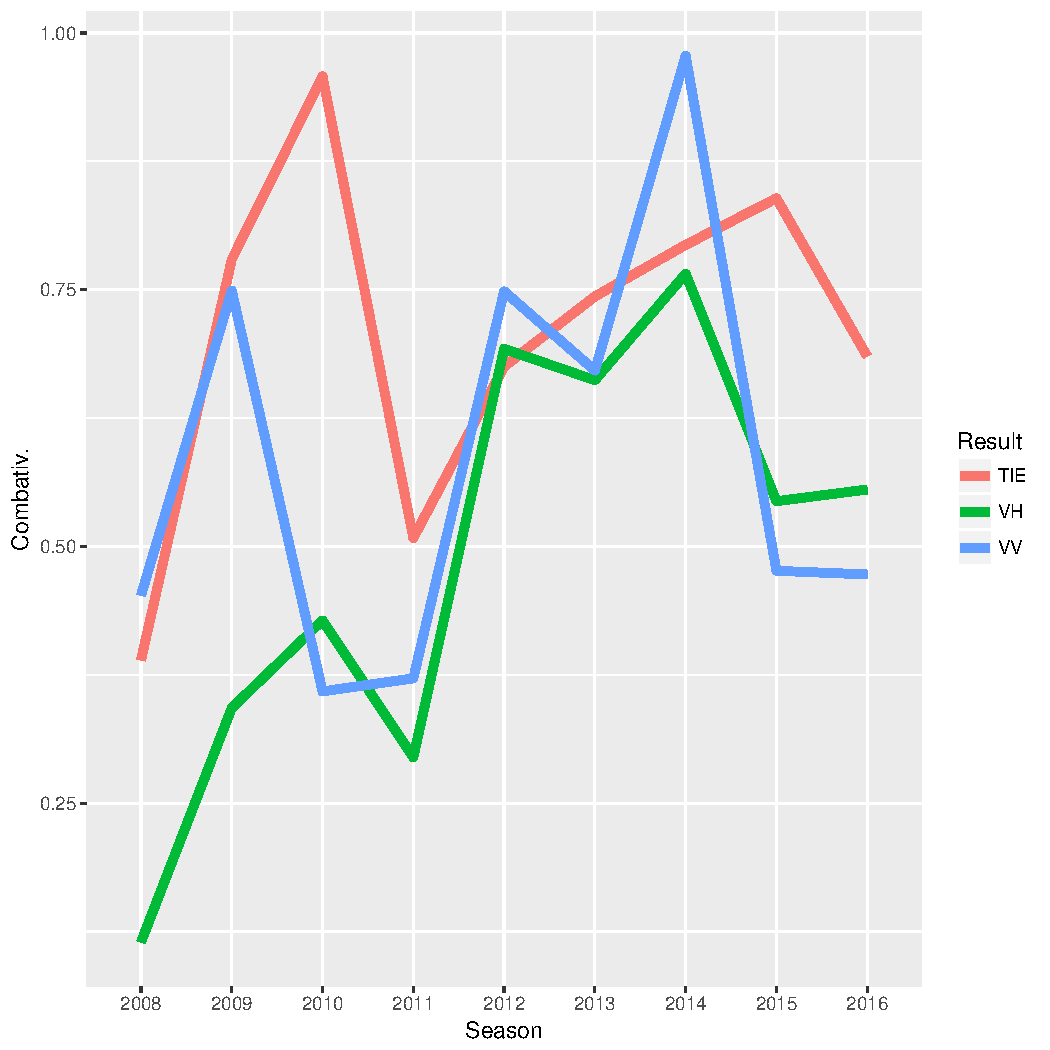
\includegraphics[width=25mm]{combativ__result_trans} &   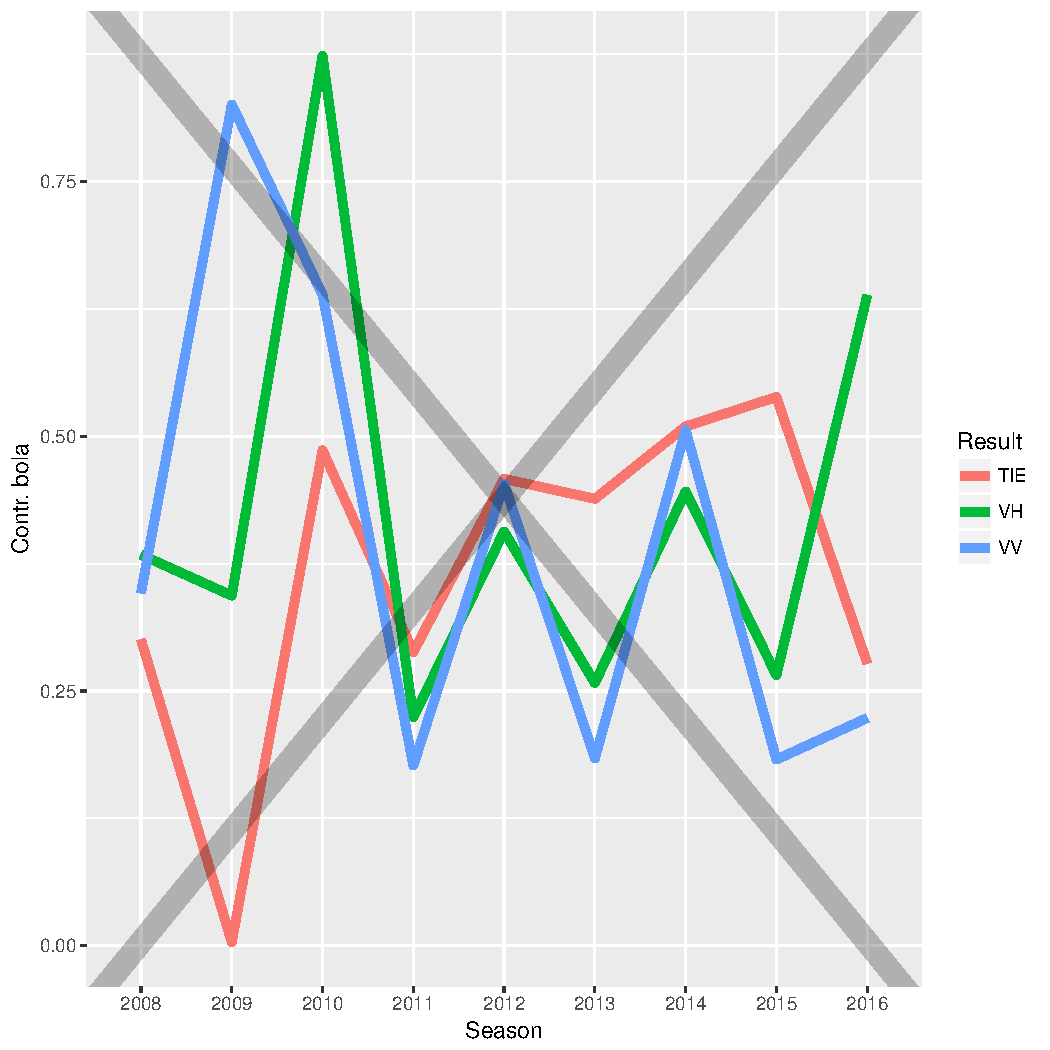
\includegraphics[width=25mm]{contr_bola_result_trans} &
  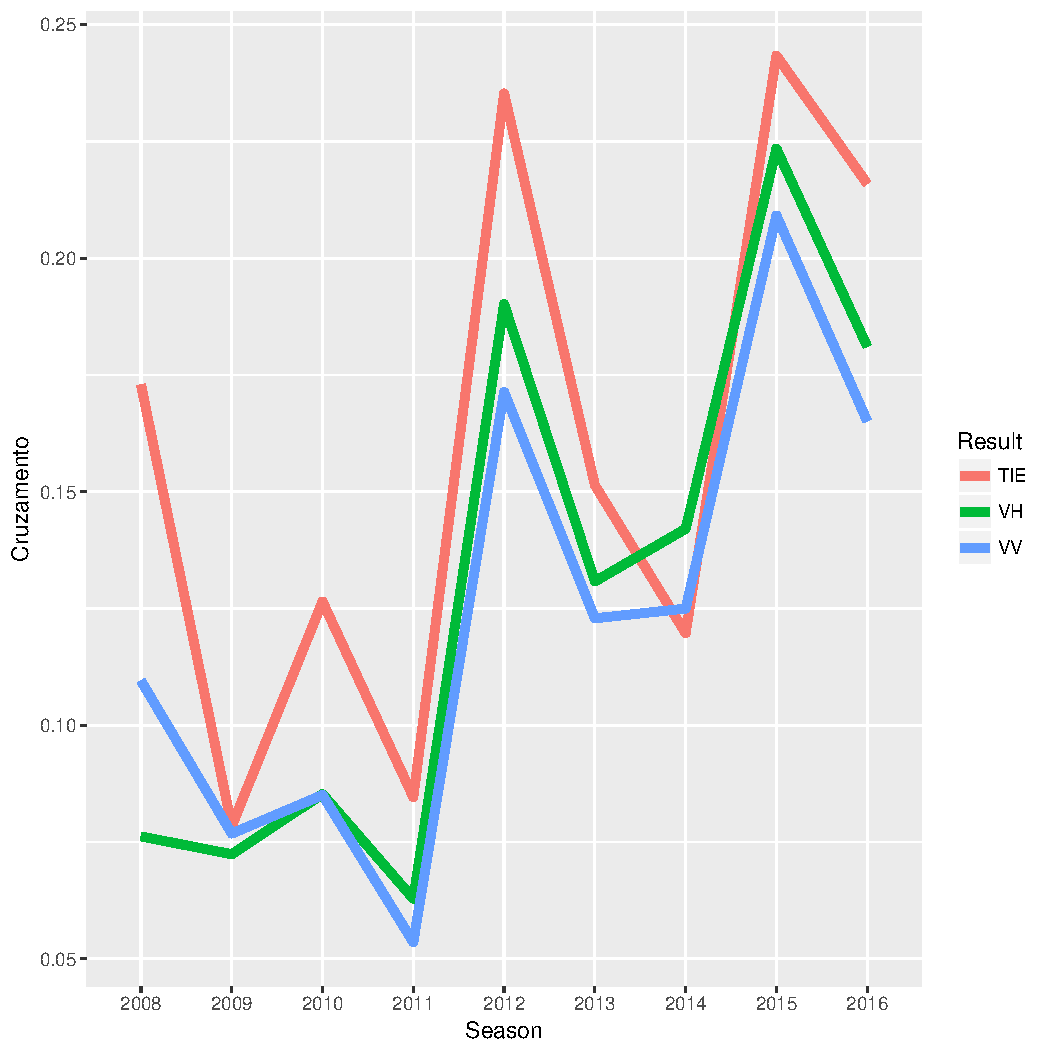
\includegraphics[width=25mm]{cruzamento_result_trans} & 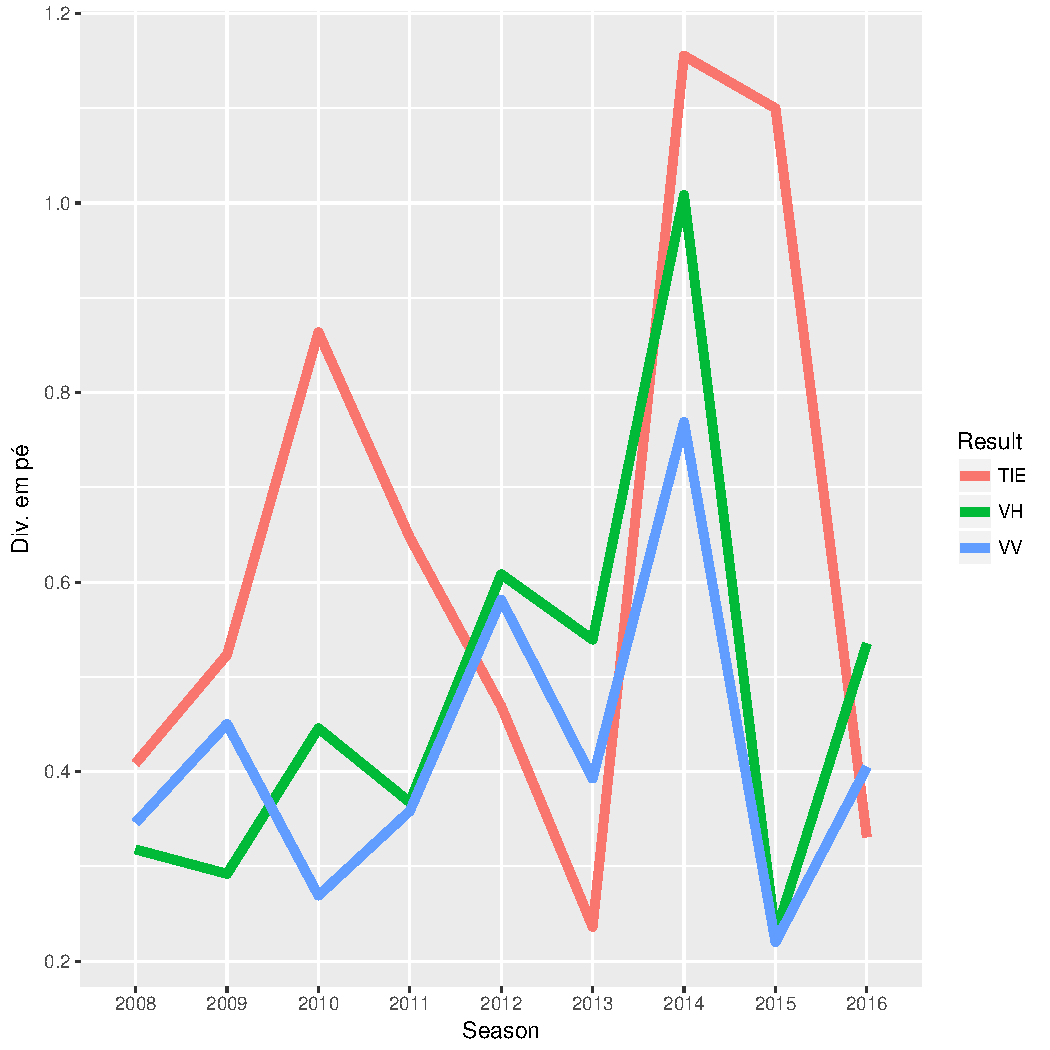
\includegraphics[width=25mm]{div_empe_result_trans} \\
 \scriptsize{(f) cobrança de falta } & \scriptsize{(g) combatividade } & \scriptsize{(h) controle de bola} & \scriptsize{(i) cruzamento} & \scriptsize{(j) dividida}\\[3pt]
 
 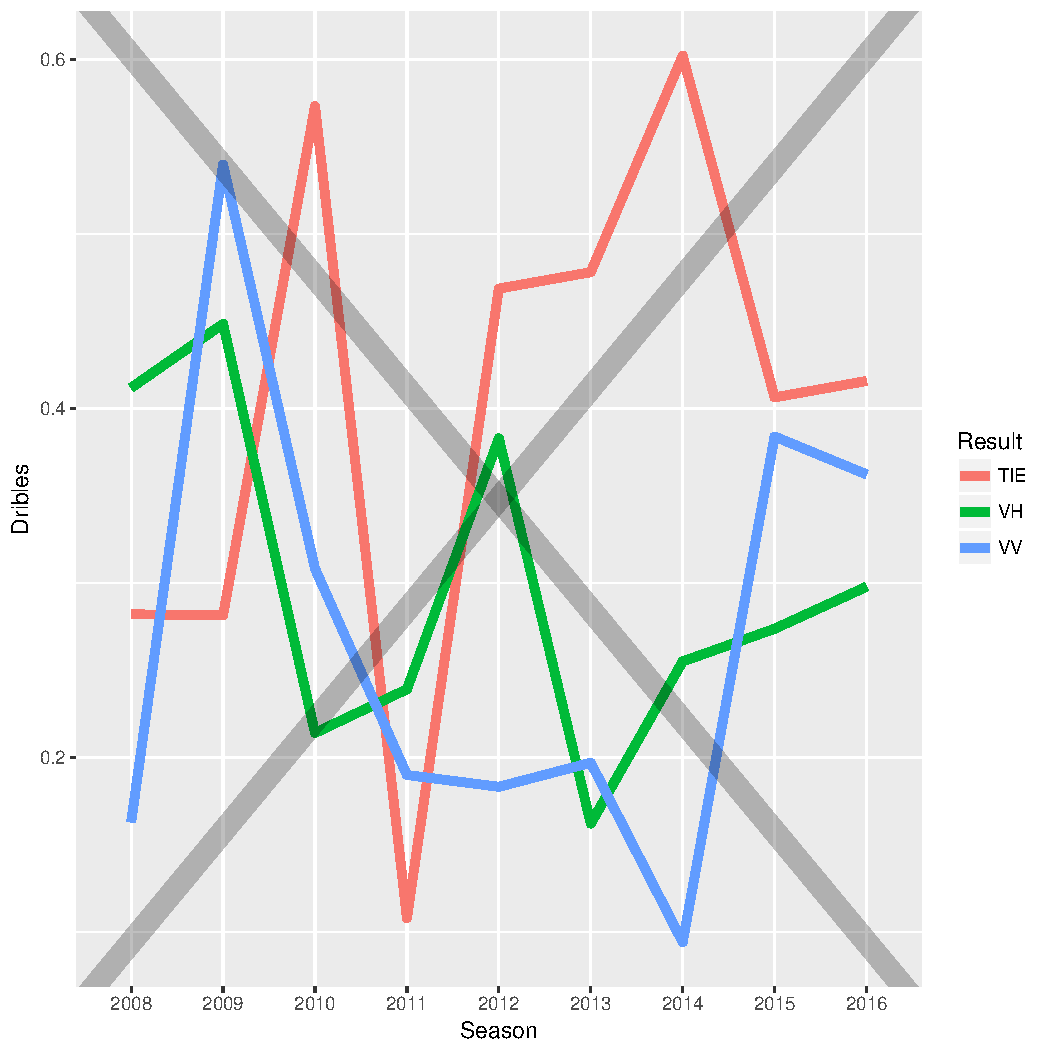
\includegraphics[width=25mm]{dribles_result_trans} & 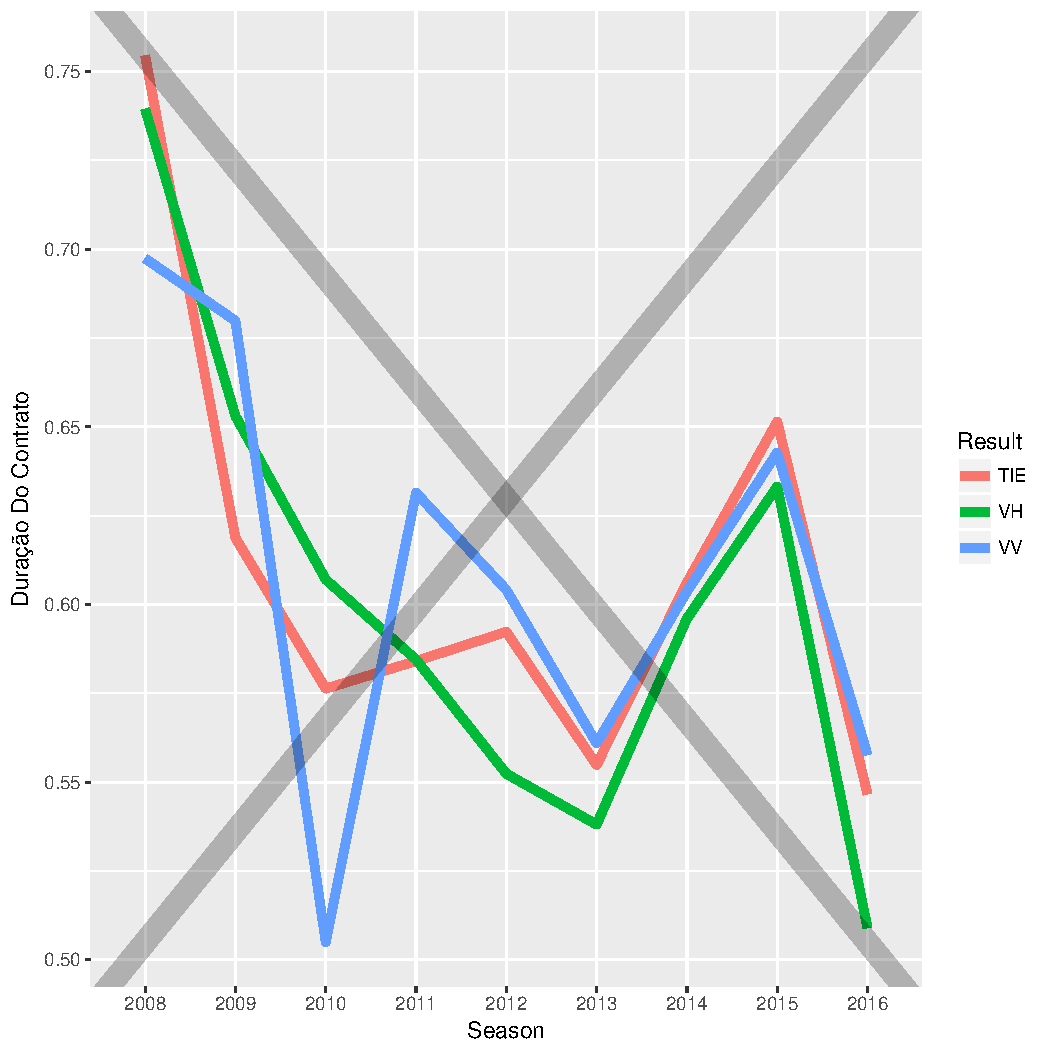
\includegraphics[width=25mm]{duracaodocontrato_result_trans} &   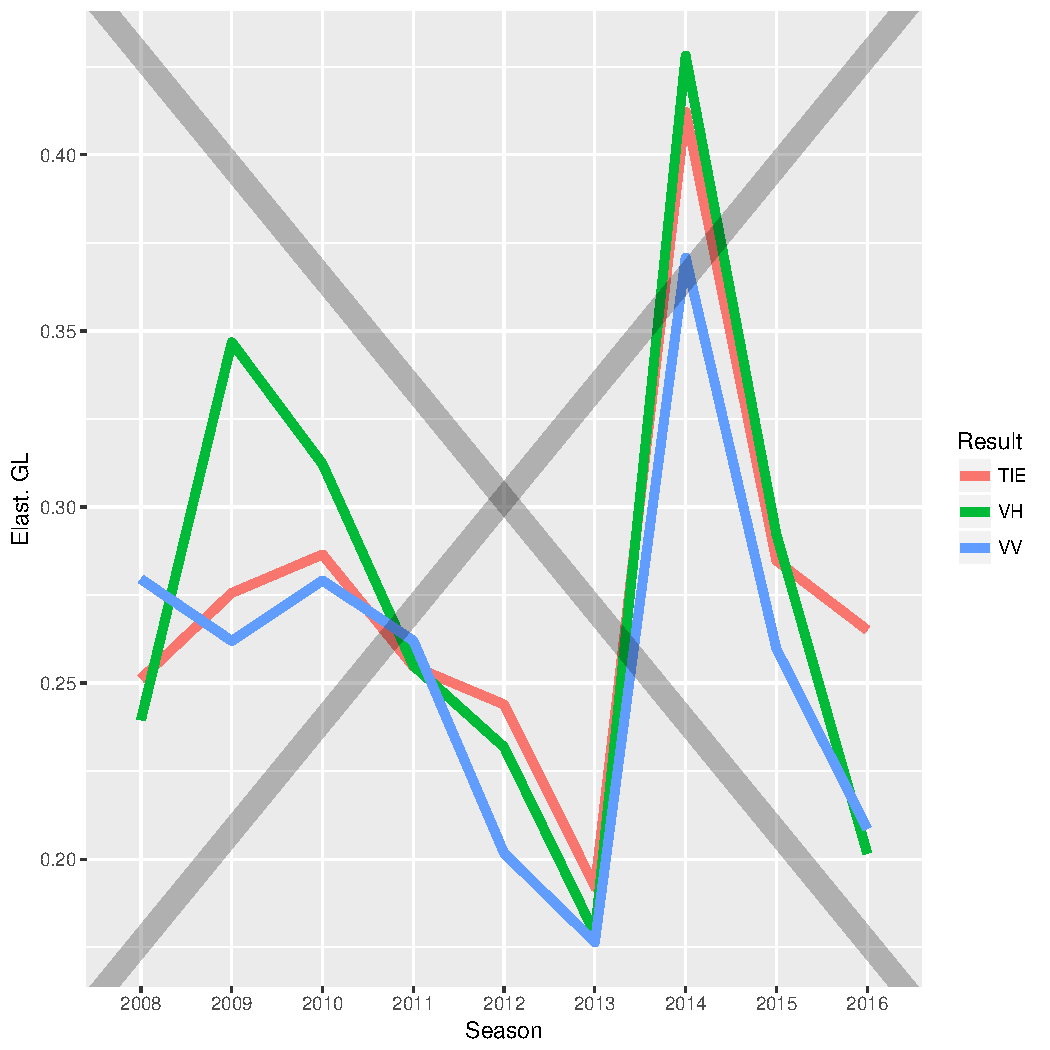
\includegraphics[width=25mm]{elast_gl_result_trans} &
  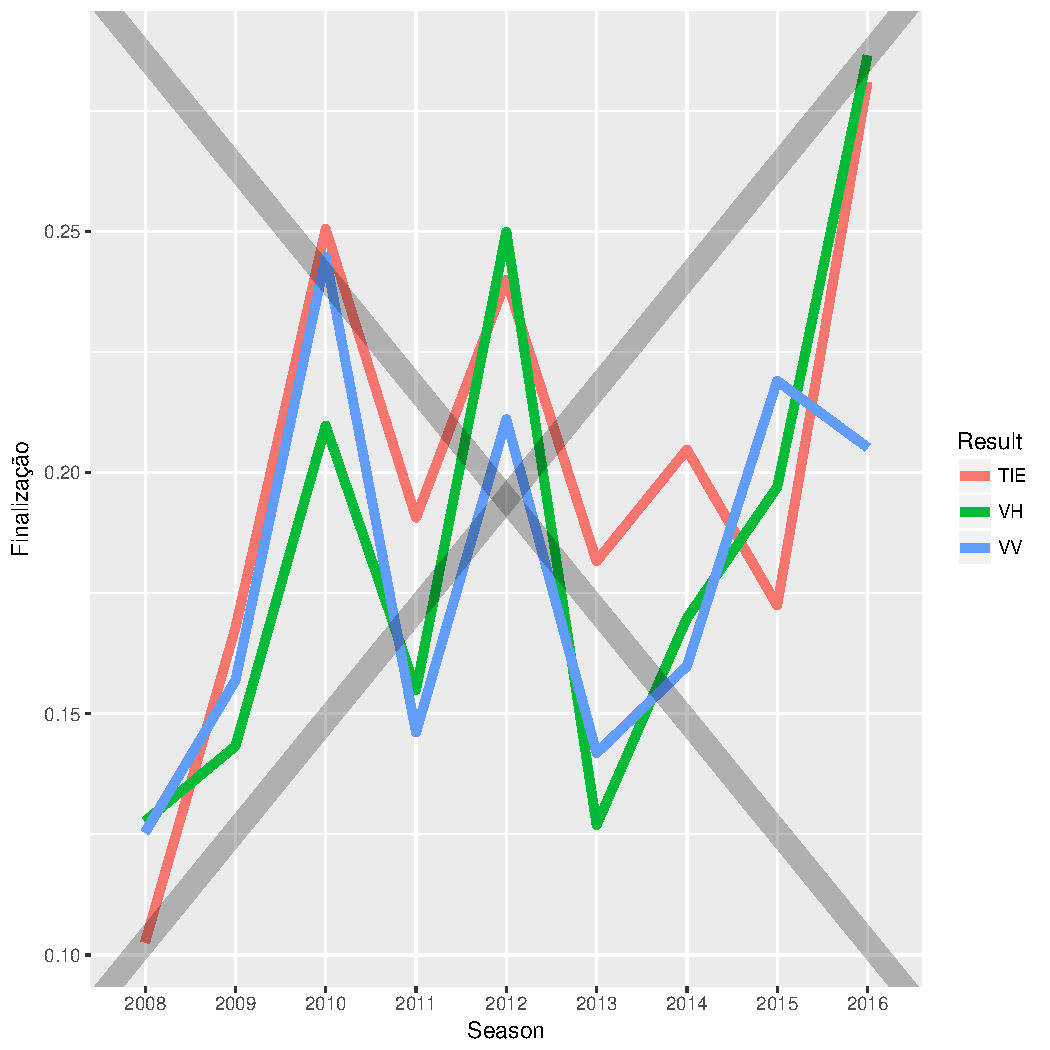
\includegraphics[width=25mm]{finalizacao_result_trans} & 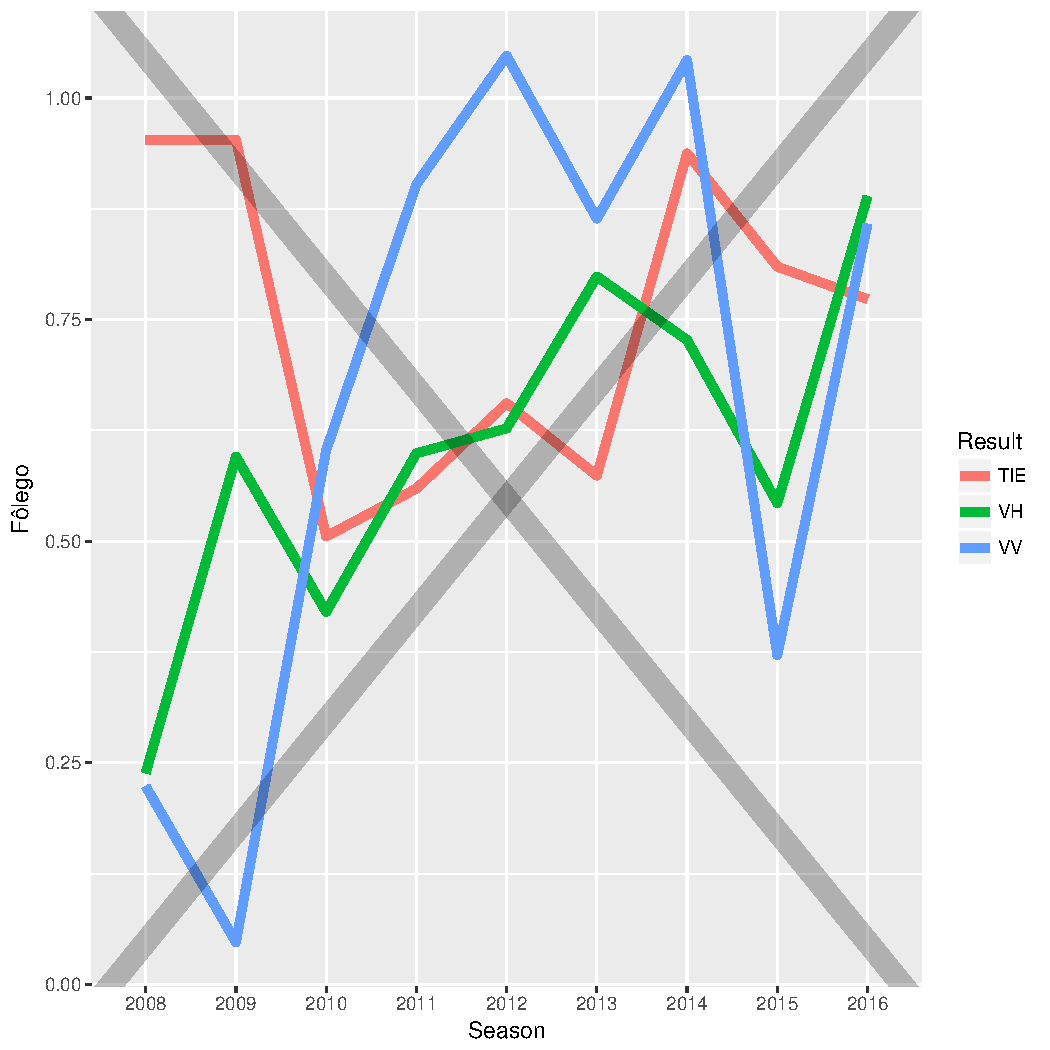
\includegraphics[width=25mm]{folego_result_trans}  \\
 \scriptsize{(k) drible} & \scriptsize{(l) duração do contrato } & \scriptsize{(m) elasticidade do goleiro} & \scriptsize{(n) finalização} & \scriptsize{(o) fôlego}\\[3pt]
 %pos_result_trans problemagrafico
  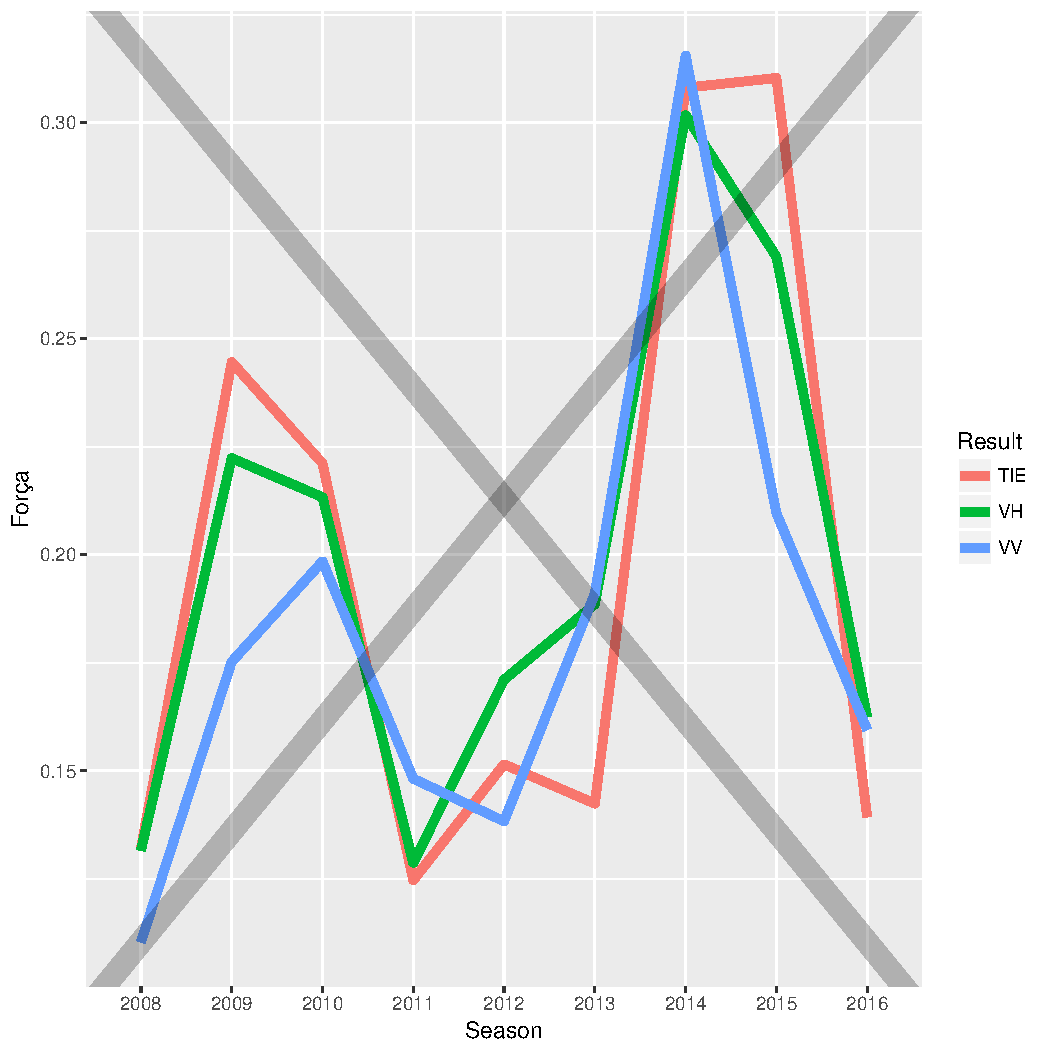
\includegraphics[width=25mm]{forca_result_trans} & \includegraphics[width=25mm]{forcachute_result_trans}  &   \includegraphics[width=25mm]{idade_result_trans} &
  \includegraphics[width=25mm]{lancamento_result_trans}  & \includegraphics[width=25mm]{manejo_result_trans}  \\
 \scriptsize{(p) força} & \scriptsize{(q) força chute } & \scriptsize{(r) idade} & \scriptsize{(s) lançamento} & \scriptsize{(t) manejo}\\[3pt]
 
   \includegraphics[width=25mm]{marcacao_result_trans} & \includegraphics[width=25mm]{passecurto_result_trans}   &   \includegraphics[width=25mm]{pernaboa_result_trans}&
  \includegraphics[width=25mm]{pernaruim_result_trans}   & \includegraphics[width=25mm]{peso_result_trans}   \\
 \scriptsize{(u) marcação} & \scriptsize{(v) passe curto } & \scriptsize{(w) perna boa} & \scriptsize{(x) perna ruim} & \scriptsize{(y) peso}\\[3pt]
 
    \includegraphics[width=25mm]{pique_result_trans}  & \includegraphics[width=25mm]{pos_result_trans_media} & \includegraphics[width=25mm]{posicion_gl_result_trans} &     \includegraphics[width=25mm]{reacao_result_trans}&
  \includegraphics[width=25mm]{reflexos_result_trans}     \\
 \scriptsize{(z) pique} & \scriptsize{(aa) posição}& \scriptsize{(ab) posição do goleiro} & \scriptsize{(ac) reação} & \scriptsize{(ad) reflexo}  \\[3pt]

\end{tabular}
    \caption[\scriptsize{Medidas resumo transformado.}]{\scriptsize{Medidas resumo transformada ao longo das temporadas para cada variável disponível. O marcador $X$ é inserido para os gráficos das variáveis não utilizadas para o modelo, por apresentar inconsistências nas relações positivas e negativas.}}
    \label{fig:medresumotrans}
\end{figure}







\begin{figure}
\begin{tabular}{ccccc}
  \includegraphics[width=25mm]{aceleracao_result_trans_media} & \includegraphics[width=25mm]{altura_result_trans_media} & \includegraphics[width=25mm]{cabeceio_result_trans_media} &   \includegraphics[width=25mm]{carrinho_result_trans_media} &
  \includegraphics[width=25mm]{ch_delonge_result_trans_media} \\
\scriptsize{(a) Aceleração } & \scriptsize{(b) altura  } & \scriptsize{(c) cabeceio } & \scriptsize{(d) carrinho } & \scriptsize{(e) chute de longe }\\[3pt]
\includegraphics[width=25mm]{cobr_falta_result_trans_media} & \includegraphics[width=25mm]{combativ__result_trans_media} &   \includegraphics[width=25mm]{contr_bola_result_trans_media} &
  \includegraphics[width=25mm]{cruzamento_result_trans_media} & \includegraphics[width=25mm]{div_empe_result_trans_media} \\
 \scriptsize{(f) cobrança de falta } & \scriptsize{(g) combatividade } & \scriptsize{(h) controle de bola} & \scriptsize{(i) cruzamento} & \scriptsize{(j) dividida}\\[3pt]
 
 \includegraphics[width=25mm]{dribles_result_trans_media} & \includegraphics[width=25mm]{duracaodocontrato_result_trans_media} &   \includegraphics[width=25mm]{elast_gl_result_trans_media} &
  \includegraphics[width=25mm]{finalizacao_result_trans_media} & \includegraphics[width=25mm]{folego_result_trans_media}  \\
 \scriptsize{(k) drible} & \scriptsize{(l) duração do contrato } & \scriptsize{(m) elasticidade do goleiro} & \scriptsize{(n) finalização} & \scriptsize{(o) fôlego}\\[3pt]
 
  \includegraphics[width=25mm]{forca_result_trans_media} & \includegraphics[width=25mm]{forcachute_result_trans_media}  &   \includegraphics[width=25mm]{idade_result_trans_media} &
  \includegraphics[width=25mm]{lancamento_result_trans_media}  & \includegraphics[width=25mm]{manejo_result_trans_media}  \\
 \scriptsize{(p) força} & \scriptsize{(q) força chute } & \scriptsize{(r) idade} & \scriptsize{(s) lançamento} & \scriptsize{(t) manejo}\\[3pt]
 
   \includegraphics[width=25mm]{marcacao_result_trans_media} & \includegraphics[width=25mm]{passecurto_result_trans_media}   &   \includegraphics[width=25mm]{pernaboa_result_trans_media}&
  \includegraphics[width=25mm]{pernaruim_result_trans_media}   & \includegraphics[width=25mm]{peso_result_trans_media}   \\
 \scriptsize{(u) marcação} & \scriptsize{(v) passe curto } & \scriptsize{(w) perna boa} & \scriptsize{(x) perna ruim} & \scriptsize{(y) peso}\\[3pt]
 
    \includegraphics[width=25mm]{pique_result_trans_media}  & \includegraphics[width=25mm]{pos_result_trans_media} & \includegraphics[width=25mm]{posicion_gl_result_trans_media} &     \includegraphics[width=25mm]{reacao_result_trans_media}&
  \includegraphics[width=25mm]{reflexos_result_trans_media}     \\
 \scriptsize{(z) pique} & \scriptsize{(aa) posição}& \scriptsize{(ab) posição do goleiro} & \scriptsize{(ac) reação} & \scriptsize{(ad) reflexo}  \\[3pt]

\end{tabular}
    \caption[\scriptsize{Medidas resumo transformado na média.}]{\scriptsize{Medidas resumo média transformada ao longo das temporadas para cada variável disponível. O marcador $X$ é inserido para os gráficos das variáveis não utilizadas para o modelo, por apresentar inconsistências nas relações positivas e negativas.}}
    \label{fig:medresumotransmedia}
\end{figure}



\section{Resultados}
\label{sec:reslt}


Comparação


\begin{figure}
\begin{tabular}{ccc}
  \includegraphics[width=55mm]{aceleracao_result} & \includegraphics[width=55mm]{aceleracao_result_trans} & \includegraphics[width=55mm]{aceleracao_result_trans_media}\\
\scriptsize{(a) Aceleração } & \scriptsize{(b) Aceleração transformado  } & \scriptsize{(c) Aceleração transformado na média} \\[3pt]

\end{tabular}
    \caption[\scriptsize{Medidas resumo transformado.}]{\scriptsize{Medidas resumo transformada ao longo das temporadas para cada variável disponível. O marcador $X$ é inserido para os gráficos das variáveis não utilizadas para o modelo, por apresentar inconsistências nas relações positivas e negativas.}}
    \label{fig:medresumcomparacao}
\end{figure}




 
Com esse critério são selecionadas as variáveis Aceleração, Cobr. falta, Contr. bola, Cruzamento, Dribles, Lançamento, Passe curto, Pique e  Reação. 

Todas as variáveis selecionadas para o modelo do empate estão no modelo de vitória ou derrota do time mandante.


% latex table generated in R 3.3.2 by xtable 1.8-2 package
% Thu Nov 16 23:42:48 2017
\begin{table}[ht]
\centering
\begin{tabular}{llrrrr}
  \hline
Seasons & Data & Global & Home & Tie & Visitor \\ 
  \hline
2008-2014 & Trainning & 53.11 & 83.05 & 1.80 & 50.43 \\ 
  2015 & Tuning & 47.11 & 83.44 & 3.74 & 37.93 \\ 
  2016 & Test & 58.16 & 84.49 & 3.57 & 55.05 \\ 
   \hline
\end{tabular}
\end{table}



% latex table generated in R 3.3.2 by xtable 1.8-2 package
% Thu Nov 16 23:53:43 2017
\begin{table}[ht]
\centering
\begin{tabular}{lrrrr}
  \hline
time & campeao & champions & europa & rebaixa \\ 
  \hline
Man City & 18.00 & 55.00 & 10.00 & 6.00 \\ 
  Man Utd & 17.00 & 51.00 & 15.00 & 0.00 \\ 
  Arsenal & 15.00 & 35.00 & 15.00 & 3.00 \\ 
  Tottenham & 14.00 & 43.00 & 18.00 & 0.00 \\ 
  Liverpool & 7.00 & 31.00 & 9.00 & 3.00 \\ 
  Newcastle & 6.00 & 21.00 & 19.00 & 13.00 \\ 
  Chelsea & 6.00 & 32.00 & 12.00 & 6.00 \\ 
  Southampton & 5.00 & 27.00 & 11.00 & 8.00 \\ 
  Everton & 4.00 & 17.00 & 10.00 & 7.00 \\ 
  Crystal Palace & 2.00 & 15.00 & 10.00 & 13.00 \\ 
  Bournemouth & 2.00 & 10.00 & 5.00 & 24.00 \\ 
  West Brom & 1.00 & 5.00 & 4.00 & 34.00 \\ 
  Swansea & 1.00 & 8.00 & 10.00 & 18.00 \\ 
  Stoke City & 1.00 & 12.00 & 12.00 & 12.00 \\ 
  Leicester & 1.00 & 9.00 & 9.00 & 8.00 \\ 
  West Ham & 0.00 & 14.00 & 14.00 & 18.00 \\ 
  Watford & 0.00 & 4.00 & 6.00 & 27.00 \\ 
  Huddersfield & 0.00 & 1.00 & 4.00 & 36.00 \\ 
  Burnley & 0.00 & 5.00 & 3.00 & 33.00 \\ 
  Brighton & 0.00 & 5.00 & 4.00 & 31.00 \\ 
   \hline
\end{tabular}
\end{table}



\section{Considerações finais}
\label{sec:conclu}
\noindent


\section*{References}
\bibliography{bibli}


\end{document}